\documentclass[a4paper, twoside]{article}
\usepackage[utf8]{inputenc} % Especifica la codificación de caracteres de los documentos.
\usepackage[spanish]{babel} % Indica que el documento se escribirá en español.
\usepackage[top=3cm, bottom=2.5cm, inner=1.5cm, outer=2.5cm]{geometry} % Márgenes personalizados
\usepackage{subfiles} % Paquete para incluir el preambulo en los sub archivos.
\usepackage{afterpage} % Permite añadir páginas despues de una página dada.
\usepackage{hyperref} % Permite incluir enlaces en los archivos.
\usepackage{lastpage} % Paquete para poder contabilizar el total de páginas del documento.
\usepackage{fancyhdr} % Permite personalizar los header y footer del documento.
\usepackage{graphicx} % Permite incluir gráficos
\usepackage[hang, bf]{caption} % Personaliza los subtítulos de las figuras y tablas
\usepackage{float} % Permite posicionar mejor las figuras y tablas
\usepackage{amsmath} % Comandos para la escritura de fórmulas matemáticas de mayor complejidad
\usepackage{amsfonts} % Proporciona fuentes matemáticas
\usepackage{amssymb} % Proporciona símbolos matemáticos de la American Mathematical Society
\usepackage{color}
\usepackage{array}
\usepackage{textcomp}
\usepackage{multirow}
\usepackage[normalem]{ulem}
\usepackage{listings}
\usepackage{listingsutf8}

% Defino la ruta de los paquetes personalizados para el apunte
\newcommand{\rutapaquetes}{./paquetes-apunte}

\usepackage[mostrarlicencia]{\rutapaquetes/caratula} % Caratula personalizada (cargada desde caratula.sty)
\usepackage{\rutapaquetes/macros} % Macros útiles para los apuntes (cargado desde macros.sty)
\usepackage[ocultarrevisores]{\rutapaquetes/colaboradores} % Seccion de colaboradores (cargada y creada con colaboradores.sty)
\usepackage{\rutapaquetes/historial} % Seccion de historial de cambios (cargada y creada con historial.sty)

% Define los estilos de los enlaces interpretados por el paquete hyperref
\hypersetup{
    colorlinks=true,   % false: boxed links; true: colored links
    linkcolor=black,   % color of internal links (change box color with linkbordercolor)
    citecolor=green,   % color of links to bibliography
    filecolor=magenta, % color of file links
    urlcolor=blue,     % color of external links
}

\newcommand{\imgdir}{../resources/images} % Ruta de las imágenes

% Define los directorios de las imágenes y gráficos
\graphicspath{ {\imgdir/} {\rutapaquetes/} }

\newcommand{\nombremateria}{Base de Datos (75.15 - 95.05)} % Defino el comando "\nombremateria" para no harcodear el nombre en varios lugares.

% Define el pagestyle personalizado
\pagestyle{fancy}
\fancyhf{}
\renewcommand{\sectionmark}[1]{\markboth{}{\thesection\ \ #1}}
% Define header para pagina par
\fancyhead[ER]{\rightmark}
% Define header para pagina impar
\fancyhead[OL]{\rightmark}
% Define footer para pagina par
\fancyfoot[EL]{\nombremateria \hspace{0.1cm} - Resumen} % Nombre del apunte a la izquierda
\fancyfoot[ER]{Página \thepage\ de \pageref{LastPage}} % Numero de pagina a la derecha
% Define footer para pagina impar
\fancyfoot[OL]{Página \thepage\ de \pageref{LastPage}} % Numero de pagina a la izquierda
\fancyfoot[OR]{\nombremateria \hspace{0.1cm} - Resumen} % Nombre del apunte a la derecha

\renewcommand{\footrulewidth}{0.4pt} % Agrego linea que separa el footer

% Configura la caratula
\materia{\nombremateria}
\tipoapunte{Resumen}
%\tema{Tema de la Materia}
%\subtema{Subtema}

%%%%%%%%%%%%%%%%%%%%%%%%%%%%%% LyX specific LaTeX commands.
%% Because html converters don't know tabularnewline
\floatstyle{ruled}
\newfloat{algorithm}{tbp}{loa}
\providecommand{\algorithmname}{Algoritmo}
\floatname{algorithm}{\protect\algorithmname}

%%%%%%%%%%%%%%%%%%%%%%%%%%%%%% User specified LaTeX commands.
\usepackage{titlesec}

\def\ojoin{\setbox0=\hbox{$\bowtie$}%
  \rule[-.02ex]{.25em}{.4pt}\llap{\rule[\ht0]{.25em}{.4pt}}}
\def\leftouterjoin{\mathbin{\ojoin\mkern-5.8mu\bowtie}}
\def\rightouterjoin{\mathbin{\bowtie\mkern-5.8mu\ojoin}}
\def\fullouterjoin{\mathbin{\ojoin\mkern-5.8mu\bowtie\mkern-5.8mu\ojoin}}

\makeatletter

\@ifundefined{showcaptionsetup}{}{%
 \PassOptionsToPackage{caption=false}{subfig}}
\usepackage{subfig}
\makeatother


\lstset{
	inputencoding=utf8,
	language=SQL,
	basicstyle={\small \ttfamily},
	keywordstyle={\color{blue}},
	commentstyle={\color{red}}
}
\renewcommand{\lstlistingname}{Listado de código}

%------------------------- Inicio del documento ---------------------------

\begin{document}

\maketitle

% Pongo el índice en una página aparte:
\tableofcontents
%\listoffigures
%\listoftables

\subfile{\rutapaquetes/acerca-del-proyecto.tex} % Inlcuye informacion acerca del proyecto FIUBA Apuntes

\part{Introducción a las Bases de Datos}

\section{Modelo de datos}
Un fenómeno o idea usualmente refiere a un objeto y a algún aspecto del objeto, el cual captura un determinado valor en un cierto momento.

\begin{description}
	\item [Dato] tupla \textless nombre de objeto, propiedad de objeto, valor de la propiedad del objeto, instante \textgreater .
	\item [Dato elemental] terna \textless nombre de objeto, propiedad de objeto, valor de la propiedad del objeto \textgreater .
	\item [Modelo de datos] herramienta intelectual que provee una interpretación del mundo real. Es un dispositivo de abstracción.
\end{description}

\begin{figure}[H]
	\noindent
	\centering
	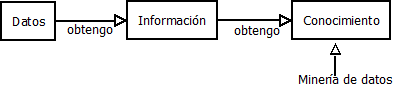
\includegraphics[scale=0.6]{datos_info_con}
	\caption{Datos, información y conocimiento}
\end{figure}

\emph{Ejemplos de modelos de representación simbólica de la información: lenguaje natural, fórmulas matemáticas, mapas, partituras.}

La pieza más elemental de información es el \textbf{dato}. Un dato solo es de utilidad si está vinculado a otros datos. La estructura y el contexto le dan significado a los datos.


\section{BDs y SGBDs}
\begin{description}
	\item [Sistema de Base de Datos] está formado por cuatro componentes:\end{description}
	\begin{enumerate}
		\item Hardware
		\item Software
		\item Datos
		\item Personas
		\begin{enumerate}
			\item \textbf{Administradores}: definen el esquema de la base de datos, definen permisos de acceso, ejecutan mantenimientos de rutina (backups, ampliando la capacidad de los discos, monitoreando la performance)
			\item \textbf{Usuarios}

\begin{tabular*}{0.9\textwidth}{@{\extracolsep{\fill}}|>{\centering}p{3cm}|>{\centering}p{5cm}|>{\centering}p{5cm}|}
	\hline 
	\textbf{Tipo de usuario} & \textbf{Descripción} & \textbf{Interfaz que utiliza} \tabularnewline
	\hline 
	\hline 
	\emph{Ingenuos} & Consultan la base de datos & Rellenando formularios de consulta, o leyendo reportes generados de la base de datos. Usan aplicaciones \tabularnewline
	\hline 
	\emph{Sofisticados} & Consultan la base de datos mediante un lenguaje, sin programar aplicaciones &
		\begin{itemize}
			\item Herramientas OLAP (\emph{Online Analytical Processing})
			\item Herramientas de \emph{data mining}
		\end{itemize} \tabularnewline
	\hline 
	\emph{Programador} \emph{de} \emph{aplicaciones} & Crean programas para acceder a la base de datos & Herramientas RAD \emph{(Rapid Application Development}) \tabularnewline
	\hline 
	\emph{Especializados} & Programan aplicaciones especiales (\emph{knowledge} \emph{bases}, sistemas expertos, etc.) & \\
	\hline 
\end{tabular*}
	\end{enumerate}
\end{enumerate}

\begin{description}
	\item[Sistema de Gestión de Base de Datos (SGBD)] \emph{Ejemplos: Oracle, MySQL, SQL Sever, DB2, Access, PosgreSQL}. Sistema formado por datos y los programas que acceden a los datos. Su objetivo es almacenar y permitir consultas en formas convenientes y eficientes.

	Está formado por tres capas, las \textbf{abstracciones}:
	\begin{enumerate}
		\item \emph{Nivel exterior}: ``vistas'' que ven los usuarios. Solo ven una parte de la base de datos, la que les interesa
		\item \emph{Nivel lógico}: cómo se agrupan lógicamente los datos, las entidades y sus relaciones. \emph{Ejemplo: tablas, grafos.}
		\item \emph{Nivel físico}: como se organizan físicamente los datos. \emph{Ejemplos: bitmaps, árboles.}
	\end{enumerate}

	\item[Gestión de Base de Datos] está formada por las siguientes herramientas:
	\begin{enumerate}
		\item \emph{Compiladores}: proveen el lenguaje de consulta.
		\item \emph{Catálogo}: provee información de la base de datos; por ejemplo, para sacar estadísticas de consultas.
		\item \emph{Optimizador de consultas}
		\item \emph{Manejador de transacciones}: asegura que una transacción se ejecute completamente o permita una vuelta atrás.
		\item \emph{Manejador de concurrencia}: asegura la integridad de la base de datos ante usuarios concurrentes.
		\item \emph{Manejador de seguridad}: 
		\begin{enumerate}
			\item Contra hechos no intencionales. \emph{Ejemplo: fallas de energía.}
			\item Contra hechos intencionales. \emph{Ejemplo: ataques de terceros para robar información.}
		\end{enumerate}
	\end{enumerate}
\end{description}

\begin{figure}[H]
	\subfloat[Los datos se almacenan en una base de datos, que es administrada por un sistema de gestión de bases de datos]
	{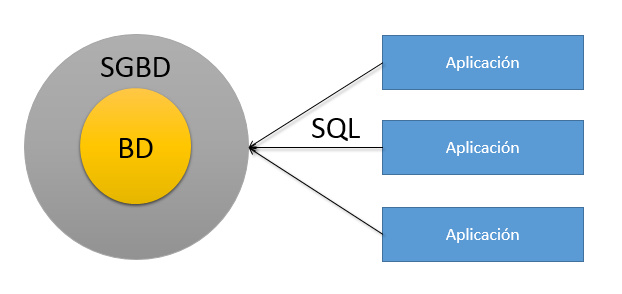
\includegraphics[width=0.5\textwidth]{bd_sgbd}}
	\subfloat[Estructura general de un sistema de base de datos]
	{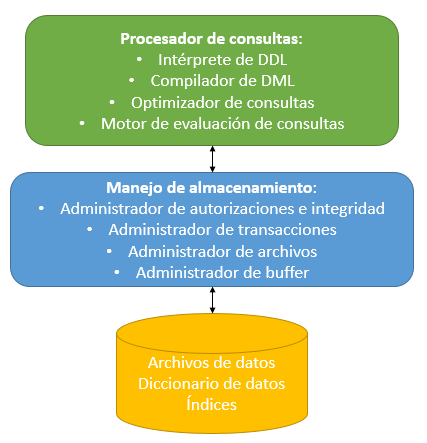
\includegraphics[width=0.5\textwidth]{estructura_bd}}
	\caption{SGBD}
\end{figure}

\subsection{Base de datos}
\begin{description}
	\item[Base de Datos (BD)] conjunto de datos interrelacionados.
	\item[Instancia de la base de datos] colección de información en la base de datos en un momento particular.
	\item[Esquema de la base de datos] descripción de la base de datos. La base de datos física varía con el tiempo (porque se producen altas, bajas y modificaciones), pero el esquema es fijo (o se cambia en raras ocasiones).
	\begin{itemize}
		\item Modelo conceptual: representación de alto nivel, que concentra los requerimientos del cliente. Utiliza el modelo Entidad-Relación.
		\item Modelo lógico: representación de bajo nivel. Utiliza el modelo relacional.
		\item Modelo físico: utiliza \textbf{SQL}.
	\end{itemize}
\end{description}

\begin{figure}[H]
	\centering
	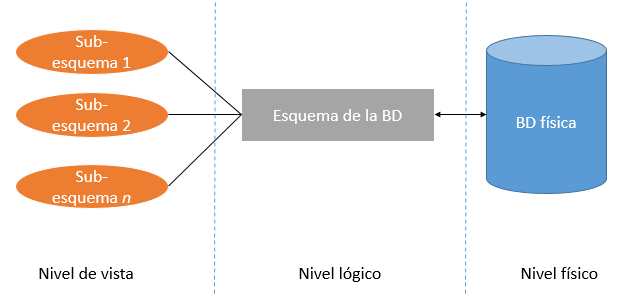
\includegraphics[scale=0.65]{esquema_bd}
	\caption{Base de datos}
\end{figure}

\subsection{¿Por qué una base de datos y no un sistema de archivo?}
Desventajas de usar un sistema de archivo:
\begin{itemize}
	\item Inconsistencia y redundancia, porque se usan muchos archivos, y tal vez tienen distintos formatos
	\item Dificultad para acceder a los datos, porque se necesitan programas para acceder a los archivos
	\item Problemas de integridad, porque es difícil cambiar todos los programas para que adopten restricciones de consistencia
	\item Dificultad para asegurar la atomicidad de las transacciones
	\item Problemas para garantizar el acceso concurrente
	\item Problemas de seguridad
\end{itemize}

\subsection{Diseño de una base de datos}
\begin{figure}[H]
	\centering
	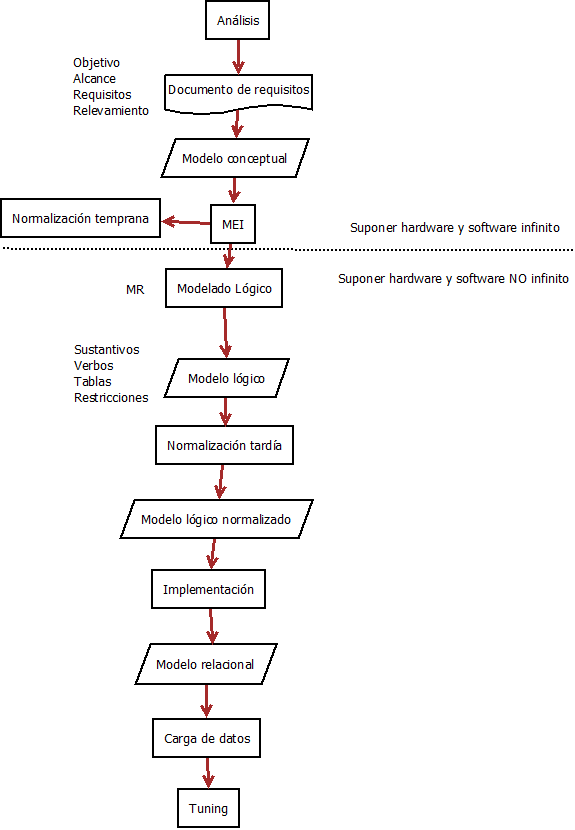
\includegraphics[scale=0.55]{diseno_bd}
	\caption{Metodología de diseño de una base de datos}
\end{figure}

\subsection{Modelos de datos}
\begin{description}
	\item[Modelo de datos] guía para organizar los datos de una base de datos. Formado por tres componentes: 
	\begin{enumerate}
		\item la \emph{estructura} de los datos (tablas, árboles, redes, etc.),
		\item las \emph{operaciones} sobre las estructuras, y
		\item las \emph{restricciones} sobre las estructuras o sobre las operaciones (para que los datos mantengan su integridad semántica).
	\end{enumerate}
\end{description}

La \textbf{potencia semántica} de un modelo de datos está determinada por su capacidad de representar, además de la estructura de los datos, el significado de los mismos y sus interrelaciones.

\subsubsection{Operaciones en una base de datos}
\begin{description}
	\item[Estado de una BD] valor de todos los atributos de todos los objetos de la base de datos.
	\item[Operadores] los hay de dos tipos:
	\begin{enumerate}
		\item De consulta (no modifican el estado de la base de datos)
		\item De actualización (modifican el estado de la base de datos)
	\end{enumerate}
	\item[Transacción] conjunto de operaciones elementales. \emph{Ejemplo: la transferencia a una cuenta.}
	\begin{lstlisting}
leer(cuenta_a)
cuenta_a <- cuenta_a + 100
escribir(cuenta_a)
leer(cuenta_b)
cuenta_b <- cuenta_b - 100
escribir(cuenta_b)
	\end{lstlisting}
\end{description}

\subsubsection{Restricciones}
Tipos de restricciones sobre una base de datos:
\begin{itemize}
	\item \textbf{Inherentes}: determinado por la estructura de la base de datos
	\item \textbf{Explícitas}: provienen del mundo real
	\item \textbf{Implícitas}: se derivan de las explícitas
	\item \textbf{De estado}: restringen los posibles valores de los atributos. \emph{Ejemplo: la edad de una persona no puede ser negativa.}
	\item \textbf{De actualización}: restringen las posibles operaciones sobre los atributos. \emph{Ejemplo: no se puede disminuir la edad de una persona.}
	\item \textbf{De entidad}: \emph{Ejemplo: no puede haber dos objetos iguales en la misma base de datos.}
	\item \textbf{De integridad referencial}: \emph{Ejemplo: no se puede referenciar a un objeto que no existe en la base de datos.}
\end{itemize}

\subsection{Modelos de bases de datos}
\begin{enumerate}
	\item Entidad-Interrelación: para el diseño conceptual
	\item Relacional: para el modelo lógico. La relaciones se representan a través de claves foráneas
	\item Jerárquico (árbol): el acceso a niveles inferiores sólo es posible a través de sus padres
	\item De red: las relaciones entre los datos se representan con referencias físicas
	\item De objetos: existe una persistencia de los objetos más allá de la existencia en memoria
\end{enumerate}

\section{Modelo Entidad-Interrelación (E-R)}
\uline{Nota importante}: no podemos tener nombres de entidades o interrelaciones repetidos.

\subsection{Entidades}
El modelo entidad-interrelación se basa en la idea de que el mundo real está compuesto por objetos (las \emph{entidades}) y las \emph{interrelaciones} que hay entre las entidades.

\begin{description}
	\item[Entidad] algo que existe, concreto o abstracto. \emph{Ejemplo: una persona Juan, la cuenta bancaria n\textdegree 4500011.}
	\item[Conjunto de entidades / tipo de entidad] conjunto de entidades del mismo tipo. \emph{Ejemplo: el conjunto de entidades ``cliente'' abarca todas las personas que tienen cuenta en un banco.}

	Un conjunto de entidades $E$ tiene un predicado asociado $p$ para probar si una entidad $e$ pertenece al conjunto.
	\[
		E = \left\{ e/p(e)\right\} 
	\]

	Los conjuntos de entidades no necesitan ser disjuntos. \emph{Ejemplo: ``animales'' y ``mamíferos'' no son disjuntos.}

	Un tipo de entidad queda definido por:
	\begin{enumerate}
		\item \textbf{Nombre}: en singular o frase simple en singular. \emph{Ejemplos: ``cliente'', ``cuenta corriente''}
		\item \textbf{Significado}: texto preciso, conciso y claro. Debe indicar, si existieran, dependencias con otros tipos de entidades
		\item \textbf{Atributos}: características de todas las entidades de ese tipo. \emph{Ejemplo: para el conjunto de entidades ``cliente'', posibles atributos son ``nombre'', ``DNI'', ``calle'', ``ciudad'', etc.} Cada atributo tiene un conjunto de \textbf{valores} permitidos, denominado el \textbf{dominio }del atributo. \emph{Ejemplo: el DNI debe ser un número positivo.} Los atributos deben ser \textbf{atómicos} (es decir, que no se pueden descomponer), y no pueden estar repetidos.

		Formalmente, un \textbf{atributo} es una función que hace corresponder un conjunto de entidades a un dominio o producto cartesiano de dominios. \emph{Ejemplo: una entidad ``empleado'' está descrita por el conjunto \{(nombre, Juan), (apellido, Cancela), (DNI, 5.678.901)\}.}

		Un atributo puede tener el valor \textbf{nulo}, por varias razones:
		\begin{enumerate}
			\item No aplica
			\item Faltante
			\item Desconocido
		\end{enumerate}

		Tipos de atributos:
		\begin{enumerate}
			\item \emph{Simple vs compuesto. Ejemplo: nombre puede descomponerse en primer nombre, segundo nombre, y apellido.}
			\item \emph{Un valor vs Multivaluado}: se repite varias veces en la entidad. \emph{Ejemplo: número de teléfono.}
			\item \emph{Derivable}: su valor puede calcularse a partir de otros atributos. Debe evitarse. \emph{Ejemplo: si tengo el atributo ``fecha de nacimiento'', ``edad'' es un atributo derivable.}
		\end{enumerate}
		\item \textbf{Identificador}: atributo o conjunto de atributos que permiten distinguir a cada entidad dentro del conjunto de entidades del mismo tipo.
	\end{enumerate}
\end{description}

\subsection{Interrelaciones}
\begin{description}
	\item[Interrelación] asociación entre dos o más conjuntos de entidades.

	\item[Conjunto de interrelaciones / tipo de interrelación] conjunto de interrelaciones del mismo tipo. Si $E_{1},E_{2},\ldots,E_{n}$ son conjuntos de entidades, entonces el conjunto de interrelaciones $R$ es un subconjunto del producto cartesiano
	\[
		\left\{ \left(e_{1},e_{2},\ldots,e_{n}\right)/e_{1}\in E_{1},e_{2}\in E_{2},\ldots,e_{n}\in E_{n}\right\} 
	\]

	donde la tupla $\left(e_{1},e_{2},\ldots,e_{n}\right)$ es una interrelación.
	\begin{figure}[H]
		\centering
		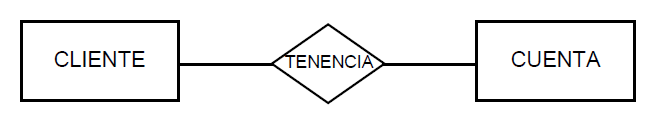
\includegraphics[scale=0.5]{er_model}
		\caption{``Tenencia'' es una interrelación entre dos entidades}
	\end{figure}

	Un tipo de interrelación puede tener atributos descriptivos. \emph{Ejemplo: la interrelación ``tenencia'' puede tener un atributo ``fecha último movimiento''.}

	Características:
	\begin{description}
		\item[Grado de una interrelación] cantidad de tipos de entidades que participan en la relación.
		\begin{figure}[H]
			\centering
			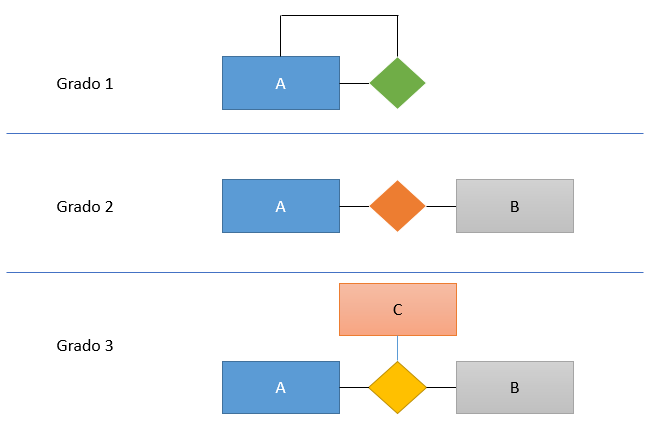
\includegraphics[scale=0.6]{grados_interrelacion}
			\caption{Grado de una interrelación}
		\end{figure}

		\item[Cardinalidad de una interrelación] cantidad de tipos de entidades con las que puede estar relacionado.
	\end{description}

	\item[Rol] función que desempeña una entidad en una interrelación. Normalmente no se especifica porque está implícito. \emph{Ejemplos: un cliente ``tiene'' una cuenta, un empleado ``es jefe de'' $n$ empleados.}
	\item[Instancia de una interrelación] asociación entre dos o más entidades. Debe ser unívocamente identificable s\emph{in usar los atributos descriptivos de la interrelación}.
\end{description}

Un tipo de interrelación puede identificarse por:
\begin{enumerate}
	\item Un atributo propio, o
	\item Una clave primaria, formada por los atributos de las claves primarias de los tipos de entidad que asocian. \emph{Ejemplo: ``DNI'' es la clave primaria de ``cliente'', y ``nro cuenta'' es la clave primaria de ``cuenta''. La clave primaria del tipo de interrelación ``tenencia'' es (DNI, nro cuenta)}
\end{enumerate}

La estructura de la clave primaria de una interrelación $R$ depende de las restricciones de cardinalidad del conjunto de interrelaciones.

\begin{figure}[H]
	\centering
	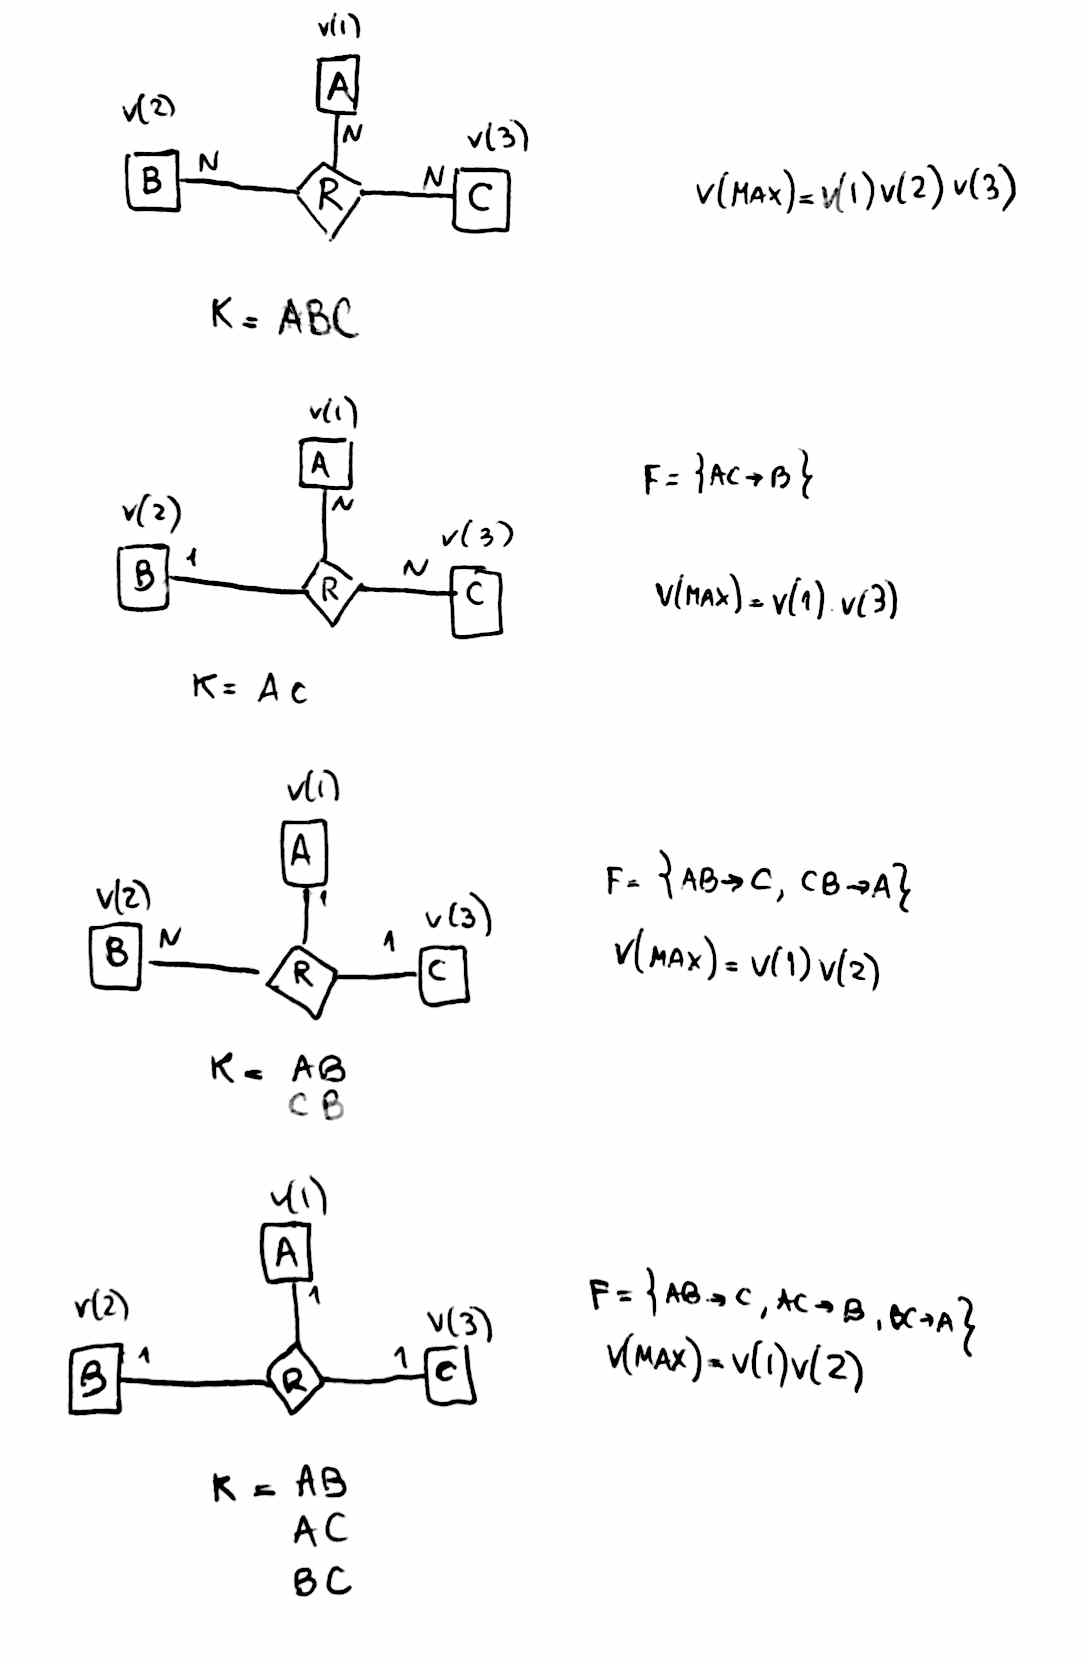
\includegraphics[scale=0.24]{interrelacion}
\end{figure}

\subsubsection{Tipos de interrelaciones}
\begin{description}
	\item[Especialización] un conjunto de entidades se divide en grupos de entidades que son distintivas. \emph{Ejemplo: en el contexto de un banco, una persona puede ser ``especializada'' en un empleado o un cliente, o ambas, o ninguna}

	\item[Generalización] la inversa de especialización. Existe una superclase y una o más subclases. 

	Puede haber restricciones de pertenencia:
	\begin{enumerate}
		\item ¿Qué tipos de entidades pueden ser miembros de una subclase?
		\begin{enumerate}
			\item Definido por condición: existe una condición o predicado explícito que decide la pertenencia o no pertenencia.
			\item Definido por el usuario: el usuario de la BD asigna entidades a una subclase.
		\end{enumerate}

		\item ¿Las entidades pueden pertenecer a más de una subclase dentro de una superclase?
		\begin{enumerate}
			\item Sí $\implies$Generalizaciones \textbf{superpuestas}
			\item No $\implies$Generalizaciones \textbf{disjuntas}
		\end{enumerate}

		\item ¿Una entidad en la superclase debe pertenecer a al menos una entidad en la subclase?
		\begin{enumerate}
			\item Sí $\implies$Generalización \textbf{total}
			\item No $\implies$Generalización \textbf{parcial}
		\end{enumerate}
	\end{enumerate}
	
	En la especialización y en la generalización, las subclases \emph{heredan atributos} de la superclase.
	
	\item[Agregación] abstracción mediante la cual un conjunto de interrelación es tratado como una superclase.
\end{description}

\subsection{Restricciones}
\subsubsection{Restricciones de participación}
Se dice que la participación de un conjunto de entidades $E$ en un conjunto de interrelaciones $R$ es \textbf{total} cuando cada entidad en $E$ participa en al menos una interrelación en $R$. Si solo algunas entidades participan, la participación es \textbf{parcial}.

\subsubsection{Restricciones de cardinalidad de correspondencia}
\textbf{Cardinalidad de correspondencia:} cantidad mínima y máxima de entidades a las cuales puede asociarse una entidad a través de un tipo de interrelación.\\

Para una interrelación \emph{binaria} $R$ entre dos tipos de entidades $A$ y $B$, la cardinalidad puede ser:
\begin{enumerate}
	\item Uno a uno $(1:1)$: Una entidad en $A$ está asociada como máximo a una entidad en $B$, y una entidad en $B$ está asociada como máximo a una entidad en $A$.
	\begin{figure}[H]
		\centering
		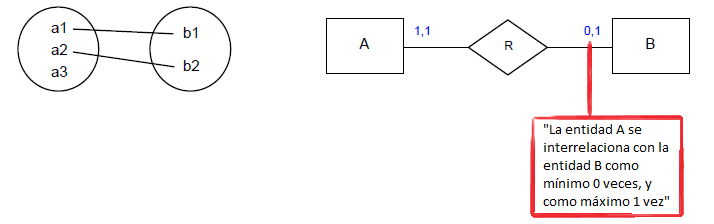
\includegraphics[width=0.8\textwidth]{cardinalidad_11}
		\caption{Cardinalidad $1:1$}
	\end{figure}

	\item Uno a muchos $(1:M)$: Una entidad en $A$ está asociada como máximo con cualquier cantidad de entidades en $B$, y una entidad en $B$ está asociada como máximo a una entidad en $A$.

	También existe la restricción ``muchos a uno'' ($M:1$).
	\begin{figure}[H]
		\centering
		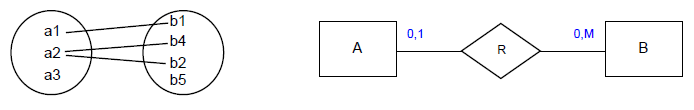
\includegraphics[width=0.8\textwidth]{cardinalidad_1M}
		\caption{Cardinalidad $1:M$}
	\end{figure}

	\item Muchos a muchos $(M:M)$: Una entidad en $A$ está asociada como máximo con cualquier cantidad de entidades en $B$, y una entidad en $B$ está asociada como máximo con cualquier cantidad de entidades en $A$.
	\begin{figure}[H]
		\centering
		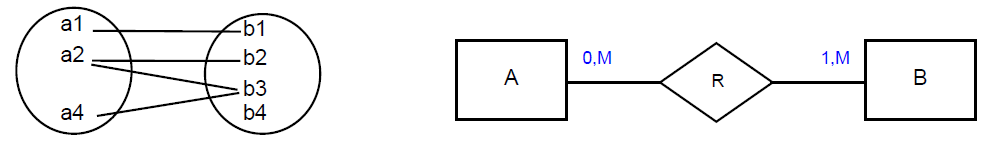
\includegraphics[width=0.8\textwidth]{cardinalidad_MM}
		\caption{Cardinalidad $M:M$}
	\end{figure}
\end{enumerate}

Para una interrelación \emph{ternaria} $R$ entre tres tipos de entidades $A,B$ y $C$, la cardinalidad puede ser:	\begin{itemize}
	\item N:N:N
	\begin{figure}[H]
		\centering
		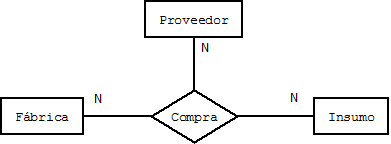
\includegraphics[scale=0.5]{ternaria_nnn}
		\caption{Las fábricas le compran insumos a proveedores.}
	\end{figure}

	Claves candidatas de ``Compra'': $\left\{ id_{f\acute{a}brica},id_{insumo},id_{proveedor}\right\} $

	\item N:N:1
	\begin{figure}[H]
		\centering
		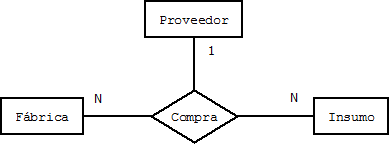
\includegraphics[scale=0.5]{ternaria_nn1}
		\caption{Las fábricas le compran insumos a proveedores. Una fábrica no puede comprar el mismo insumo a más de un proveedor.}
	\end{figure}

	Claves candidatas de ``Compra'': $\left\{ id_{f\acute{a}brica},id_{insumo}\right\} $

	\item N:1:1
	\begin{figure}[H]
		\centering
		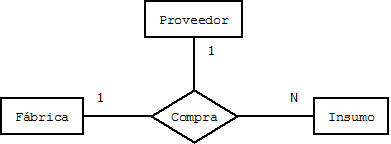
\includegraphics[scale=0.5]{ternaria_n11}
		\caption{Las fábricas le compran insumos a proveedores. Una fábrica no puede comprar el mismo insumo a más de un proveedor. Un proveedor no puede venderle el mismo insumo a más de una fabrica.}
	\end{figure}

	Claves candidatas de ``Compra'': $\left\{ id_{f\acute{a}brica},id_{insumo}\right\} ;\left\{ id_{proveedor},id_{insumo}\right\} $

	\item 1:1:1
	\begin{figure}[H]
		\centering
		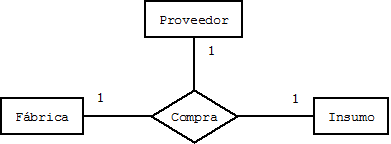
\includegraphics[scale=0.7]{ternaria_111}
		\caption{Las fábricas le compran insumos a proveedores. Una fábrica no puede comprar el mismo insumo a más de un proveedor. Un proveedor no puede venderle el mismo insumo a más de una fabrica. Una fábrica no puede comprarle más de un insumo a cada proveedor.}
	\end{figure}

	Claves candidatas de ``Compra'': $\left\{ id_{f\acute{a}brica},id_{insumo}\right\} ;\left\{ id_{proveedor},id_{insumo}\right\} ;\left\{ id_{f\acute{a}brica},id_{proveedor}\right\} $
\end{itemize}

\textbf{Teorema:} en las relaciones ternarias, las restricciones de cardinalidad no imponen restricciones en las relaciones binarias. \emph{En el ejemplo anterior, una fábrica puede comprar $N$ insumos. Una fábrica puede comprarle a $N$ proveedores. Un proveedor puede proveer $N$ insumos.}

\subsubsection{Restricciones de dependencia existencial}
Si la existencia de la entidad $S$ depende de la existencia de la entidad $D$, entonces se dice que $S$ tiene \textbf{dependencia existencial} de $D$. Operacionalmente, esto significa que si $D$ es borrado, también $S$ es borrado. La entidad $D$ es la entidad \textbf{dominante} y $S$ es la entidad \textbf{subordinada}.

\subsubsection{Restricciones de identificación}
\begin{description}
	\item[Superclave] conjunto de uno o más atributos que, tomados en conjunto, permiten identificar unívocamente una entidad o una interrelación en el conjunto de entidades o interrelaciones del mismo tipo.

	Si $K$ es una superclave, cualquier superconjunto de $K$ también es una superclave.

	\item[Clave candidata] superclaves minimales; aquellas para las cuales ningún subconjunto propio es una superclave.

	Sea $R$ un esquema de relación con atributos $A_{1},\dots,A_{n}$. El conjunto de atributos $K=\left(A_{1},\dots,A_{k}\right)$ es una clave candidata de $R$ sí y sólo sí satisface:
	\begin{enumerate}
		\item \emph{Unicidad}: en todo momento, no existen dos tuplas distintas de $R$ que tengan el mismo valor para $A_{i}$, donde $i\in[1,k]$.
		\item \emph{Minimalidad}: ningún atributo de $K$ puede ser eliminado sin que se pierda la propiedad de unicidad.
	\end{enumerate}

	\item[Clave primaria] aquella clave candidata que es elegida por el diseñador del modelo de datos para identificar entidades dentro del conjunto de entidades. Esta clave no debería cambiar en el tiempo. \emph{Ejemplo: la dirección de un cliente no es una buena clave primaria, porque se puede mudar}

	\item[Clave foránea] atributo o conjunto de atributos que es clave primaria en otra relación. \emph{Ejemplo: en una relación ``autos'', puede haber una clave foránea ``DNI'' que es la clave primaria en otra relación ``personas'', y que indica el dueño de ese auto}

	\item[Entidad débil] entidad que tiene \textbf{dependencia de identificación}, porque no es identificable por sus propios atributos. Está subordinada a otro tipo de entidad, la entidad fuerte.

	\item[Entidad fuerte] entidad que tiene una clave primaria propia.

	El concepto de entidades fuertes y débiles está relacionado con el concepto de dependencia de existencia. Una entidad débil es, por definición, una entidad subordinada a la entidad dominante de la cual depende su identidad. Toda dependencia de identidad es una dependencia de existencia, pero una dependencia de existencia no implica necesariamente una dependencia de identidad.

	\item[Discriminador] atributo o conjunto de atributos de una entidad débil que lo distingue de otras entidades débiles que dependen de la misma entidad fuerte.
	
	Para una entidad débil, su clave primaria está formada por su identificador más la clave primaria de la entidad fuerte de la cual depende.
\end{description}

\subsection{Diagramas E-R}
\begin{figure}[H]
	\centering
	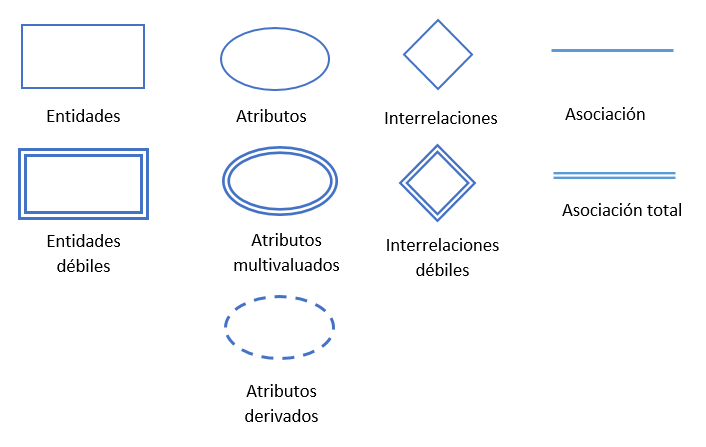
\includegraphics[scale=0.7]{simbologia_er}
	\caption{Simbología en los diagramas E-R}
\end{figure}

\begin{figure}[H]
	\centering
	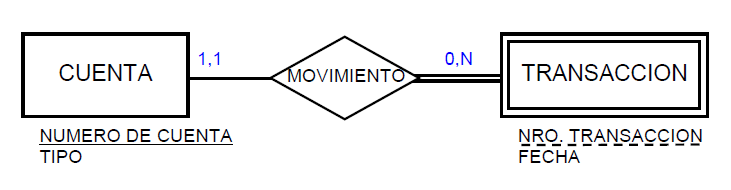
\includegraphics[scale=0.5]{simbologia_er_2}
	\caption{Simbología en los diagramas E-R para entidades fuertes (\emph{cuenta}) y débiles (\emph{transacción}). La clave primaria de la entidad fuerte se identifica con el atributo subrayado (\emph{nro. cuenta}). La dependencia a la entidad fuerte se identifica con arcos dobles. El discriminador de la entidad débil se identifica con el atributo subrayado a medias (\emph{nro. transacción}). El identificador de la entidad débil es la suma de su discriminador y de la clave primaria de la entidad fuerte (\emph{nro. cuenta + nro. transacción})}
\end{figure}

\subsection{Cuestiones de diseño}
\begin{enumerate}
	\item ¿Conjuntos de entidades vs. Atributos?
	\begin{enumerate}
		\item Algunos atributos no pueden transformarse en entidades. \emph{Ejemplo: el nombre de una persona}
		\item Algunos atributos están mejor representados como entidades, para permitir atributos. \emph{Ejemplo: teléfonos de una persona}
	\end{enumerate}

	\item ¿Conjuntos de entidades vs. Conjuntos de interrelaciones?

	Las interrelaciones modelan ``acciones'' que ocurren entre entidades.

	\item ¿Conjuntos de interrelaciones binarias vs. n-arias?

	\textbf{Teorema:} es posible reemplazar cualquier conjunto de interrelaciones $n-$aria (con $n>2$) con un número de interrelaciones binarias.

	\item Localización de atributos de interrelaciones
	\begin{enumerate}
		\item Relaciones $1:1$ $\implies$ en cualquiera de las dos entidades participantes
		\item Relaciones $1:N$ $\implies$ en la segunda entidad
		\item Relaciones $N:N$ $\implies$ en la interrelación
	\end{enumerate}
\end{enumerate}

\subsection{Reducción de un esquema E-R a un modelo relacional}
Para cada entidad y para cada interrelación, se construye una única tabla. Cada tabla contiene múltiples columnas.

\begin{itemize}
	\item Representación de conjuntos de entidades fuertes

	Sea $E$ un conjunto de entidad fuerte con atributos $a_{1},\ldots,a_{n}$. Se representa a la misma con una tabla llamada $E$ con $n$ columnas. Cada fila de la tabla es una entidad. El conjunto de todas las posibles filas de la tabla es el \textbf{producto cartesiano }entre los dominios de cada atributo:
	\[
		D_{1}\times\ldots\times D_{n}
	\]

	\item Representación de conjuntos de entidades débiles

	Sea $A$ un conjunto de entidad débil con atributos $a_{1},\ldots,a_{m}$. Sea $B$ el conjunto de entidad fuerte del cual depende $A$. La clave primaria de $B$ está formada por los atributos $b_{1},\ldots,b_{n}$. Se representa a $A$ con una tabla con $m+n$ columnas $a_{1},\ldots,a_{m},b_{1},\ldots,b_{n}$.

	\item Representación de conjuntos de interrelaciones

	Sea $R$ un conjunto de interrelaciones entre las entidades $E_{1},\dots,E_{n}$ con atributos $r_{1},\ldots,r_{m}$. Sean $a_{1},\ldots,a_{n}$ el conjunto de atributos formado por la unión de las claves primarias de cada entidad participante. Se representa a $R$ con una tabla con columnas $a_{1},\ldots,a_{n},r_{1},\ldots,r_{m}$.
	
	\emph{Si la interrelación relaciona un conjunto de entidades débil y otro fuerte, la tabla de $R$ no es necesaria, es redundante.}

	\item Representación de interrelaciones $1:N$ entre entidades $A$ y $B$

	\emph{Si la participación de $A$ en $R$ es total (i.e. cada entidad en $A$ debe participar en la relación $R$), se pueden unir las tablas de $A$ y $R$.}

	\item Representación de atributos compuestos

	Sea el atributo compuesto $x$ formado por $x_{1},\ldots,x_{n}$. Se debe generar una columna para cada $x_{1},\ldots,x_{n}$, pero \emph{no} para $x$.

	\item Representación de atributos multivaluados

	Sea el atributo multivaluado $x$. Se debe crear una tabla $T$ con una columna $C$ que corresponde a $x$ y el resto de las columnas son la clave primaria del conjunto de entidades o interrelación del cual $x$ es un atributo.

	\item Representación de generalización

	Hay dos métodos:
	\begin{enumerate}
		\item Una tabla para la superclase + una tabla para cada subclase, que incluya una columna con la clave primaria de la superclase
		\item Si la generalización es disjunta y completa, no se crea una tabla para la superclase. Se crea una tabla para cada subclase, que incluya todos los atributos de la superclase.
	\end{enumerate}

	\item Representación de agregación

	La tabla de la interrelación $R$ entre la agregación $A$ y el conjunto de entidades $B$ incluye una columna por cada clave primaria de $B$ y $A$.
\end{itemize}

\section{Modelo Relacional}
\subsection{Estructura del modelo relacional}
El modelo relacional es un ejemplo de modelo basado en registros. Usa un grupo de tablas para representar los datos y las relaciones entre los datos. Cada tabla tiene múltiples columnas. Cada tabla contiene registros de un tipo en particular. Cada registro tiene atributos (las columnas).

\begin{figure}[H]
	\centering
	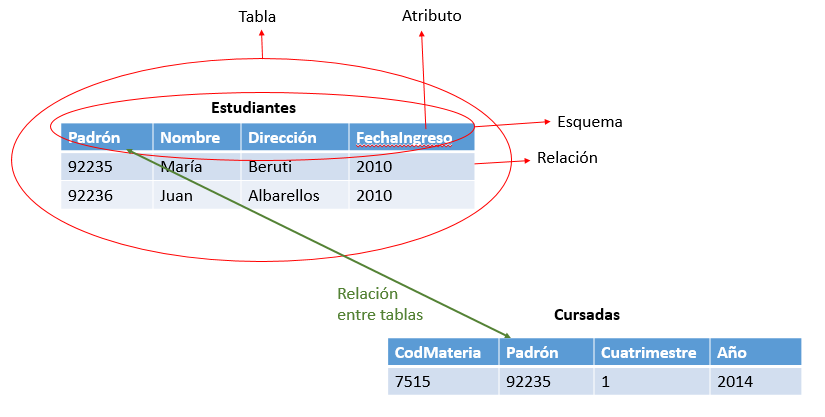
\includegraphics[scale=0.7]{tablas}
	\caption{Tablas}
\end{figure}

\begin{description}
	\item[Dominio] valores posibles de un conjunto. \emph{Ejemplo: $D_{padron}=\{1,2,\dots100000\}$}

	Existe un valor que es posible en cualquier dominio: el valor \textbf{nulo}. Este valor significa ``atributo desconocido'' o ``atributo inexistente''. Se puede prohibir, para un atributo, que este tenga el valor nulo, ya que puede causar problemas al realizar consultas.

	\item[Esquema de relación] descripción de una relación. Es el nombre de la relación seguido de la lista de los atributos con sus dominios. \emph{Ejemplo: Estudiante (Padrón, nombre, dirección, fechaIngreso)}

	\item[Relación] instancia de un esquema. Subconjunto del producto cartesiano de una lista de dominios\emph{. }Sea el esquema de relación $R$, denotamos a la instancia $r$ mediante $r(R)$.

	\item[Tabla] representación de una relación. Se pueden relacionar entre sí al compartir atributos. Una tabla de $n$ atributos es un subconjunto de $D_{1}\times D_{2}\times\dots\times D_{n}$. Notar que al ser un conjunto, el orden no interesa.

	\item[Atributo] nombre de cada columna de una tabla.

	\item[Esquema de BD relacional] conjunto de esquemas de relación.

	\item[Tupla] miembro de una relación. Son las filas de una tabla.
\end{description}

\subsection{Restricciones del modelo relacional}
\begin{itemize}
	\item Regla de integridad de entidad

	Ningún atributo de la clave primaria de un esquema de relación puede tomar valor nulo.

	\item Regla de integridad referencial

	Si la relación $r$ incluye una clave foránea $F$ que es la clave primaria $P$ de una relación $s$, entonces todo valor de $F$ en $r$ debe ser totalmente nulo o ser igual al valor de $P$ en alguna tupla de $s$.
\end{itemize}

\subsection{Operaciones del modelo relacional: álgebra relacional}
Es un lenguaje\textbf{ formal }y \textbf{procedural }que\textbf{ }permite realizar consultas sobre un conjunto de relaciones, y produce relaciones como resultado.

\subsubsection{Operadores básicos}
Los siguientes operadores son linealmente independientes. Se utilizan para filtrar,\emph{ }cortar y combinar relaciones.

\begin{enumerate}
	\item Operaciones unarias:
	\begin{enumerate}
		\item \textbf{Proyección} ($\pi_{a_{1},\dots,a_{n}}(r)$). 

		Dados los atributos $a_{1},\dots,a_{n}$ que pertenecen a $r$, devuelve una relación de esquema $\{a_{1},\dots,a_{n}\}$.

		Se eliminan las tuplas repetidas.

		\item \textbf{Selección} ($\sigma_{p}(r)$). 

		Devuelve una relación $r'$ con el mismo esquema que $r$, en la que las tuplas son aquellas pertenecientes a $r$ que satisfacen la condición o el predicado $p$. La condición puede ser de dos estilos:
		\begin{enumerate}
			\item \emph{Atómica}: expresión lógica simple del tipo que utiliza un operador de comparación $\theta$, tal que $\theta\in\left\{ =,\neq,<,>,\leq,\geq\right\} $. Se permiten dos tipos de expresiones:
			\begin{enumerate}
				\item Atributo $\theta$ atributo
				\item Atributo $\theta$ constante
			\end{enumerate}

			\item \emph{Compuesta}: utiliza conectores \emph{and, or, not}.
		\end{enumerate}

		\item \textbf{Renombre} ($\rho_{R(A_{1},A_{2},\dots,A_{n})}(E)$). 

		Cambia el nombre de la relación $E$ a $R$, y también cambia el nombre de sus atributos a $A_{1},A_{2},\dots,A_{n}$.
	\end{enumerate}

	\item Operaciones binarias:
	\begin{enumerate}
		\item \textbf{Unión} ($r\bigcup s$).

		Sean $r$ y $s$ instancias \emph{homogéneas}%
		\footnote{Las relaciones homogéneas tienen: (a) la misma cantidad de atributos, y (b) para todo $i$, el dominio del atributo $i$ de $r$ es el mismo que el dominio del atributo $i$ de $s$}%
		de las relaciones $R$ y $S$ respectivamente. $r$ contiene $m$ tuplas y $s$ contiene $n$ tuplas. La unión se define como:
		\[
			r\bigcup s=\left\{ x:\, x\in r\vee x\in s\right\} 
		\]

		Las tuplas repetidas se eliminan.

		\item \textbf{Diferencia} ($r-s$).

		Sean $r$ y $s$ instancias \emph{homogéneas }de las relaciones $R$ y $S$ respectivamente. La diferencia se define como:
		\[
			r-s=\left\{ x:\, x\in r\wedge x\not\in s\right\} 
		\]

		\item \textbf{Producto cartesiano} ($r\times s$). 

		Sean $r$ y $s$ instancias de las relaciones $R$ y $S$ respectivamente. El producto cartesiano es el conjunto de tuplas que resulta de concatenar cada tupla de $r$ con cada tupla de $s$.
		\[
			r\times s = \left\{ \left(r_{1},s_{1}\right);\ldots;\left(r_{1},s_{m}\right);\ldots;\left(r_{n},s_{1}\right)\ldots,\left(r_{n},s_{m}\right)\right\} 
		\]

		Si $r$ tiene $n$ tuplas y $s$ tiene $m$ tuplas, $r\times s$ tendrá $n\cdot m$ tuplas. El grado de $r\times s$ es la suma de los grados de $r$ y $s$.
	\end{enumerate}
\end{enumerate}

\subsubsection{Operadores secundarios}
No proporcionan nuevas funcionalidades, solo simplifican las consultas.

\begin{enumerate}
	\item \textbf{Intersección} ($r\bigcap s$)

	Dadas las relaciones $r_{1}$ y $r_{2}$ con el mismo esquema, devuelve una relación $r$ con igual esquema, tal que $r=\left\{ x:\, x\in r_{1}\wedge x\in r_{2}\right\} $
	\[
		r\bigcap s\equiv r-\left(r-s\right)
	\]

	\item \textbf{Junta (}\textbf{\emph{join}}\textbf{) ($r\bowtie s$)}

	La junta de dos relaciones $r$ y $s$ según un predicado $P$ es una relación de esquema igual al producto cartesiano $r\times s$, cuyas tuplas son el conjunto de tuplas de $r\times s$ que satisfacen
el predicado $P$.
	\[
		r\bowtie_{p}s\equiv\sigma_{p}\left(r\times s\right)
	\]

	\begin{enumerate}
		\item \textbf{\emph{Equi-join}}: dadas las relaciones $r$ y $s$, es el \emph{join} según el predicado $r.A_{i}=s.A_{j}$
		\item \textbf{\emph{Auto-join}}: dada la relación $r$, es el \emph{join} de $r$ consigo mismo según el predicado $1.A_{i}\,\theta\,2.A_{i}$ donde $1$ y $2$ son aliases de $r$.
		\item \textbf{\emph{Natural join}}\textbf{ }($r*s$). Requiere que haya atributos compartidos entre las relaciones $r$ y $s$, y además que $R\bigcap S\neq\emptyset$.
		\[
			r*s \equiv \pi_{R\cup S} \left( \sigma_{r.c_{1} = s.c_{1} \wedge r.c_{2} = s.c_{2} \wedge \dots \wedge r.c_{h} = s.c_{h}} \left( r\times s \right) \right)
		\]

		El \emph{join} natural es una operación asociativa, por lo tanto, $(r*s)*t = r*(s*t)$.
	\end{enumerate}
	
	\begin{figure}[H]
		\centering
		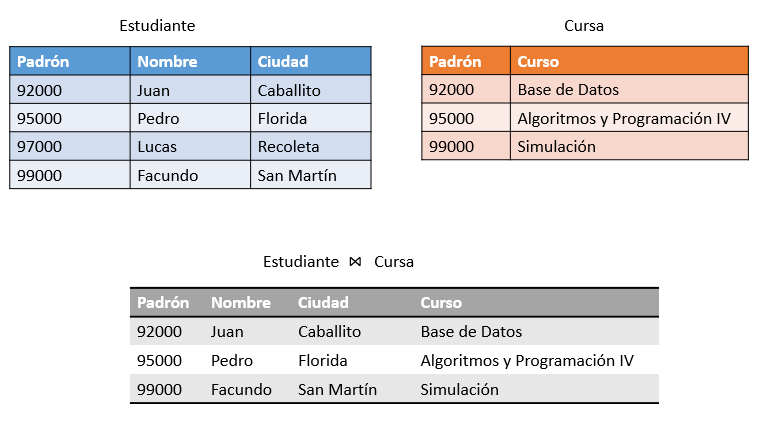
\includegraphics[scale=0.7]{join_natural}
		\caption{Junta natural}
	\end{figure}

	\item \textbf{División} ($r/s$). 

	Sean las relaciones $r\in R$ con $n$ atributos y $s\in S$ con $m$ atributos, tal que $m<n$ y $S\subset R$. La división son todas las tuplas $t$ tales que, multiplicadas por \textbf{todas} las filas $u$ de $s$, me dan filas que están en $r$. El esquema de la división es $R-S$.
	\[
		r/s\equiv\pi_{1,\dots,n-m}(r)-\pi_{1,\dots,n-m}\left(\left(\pi_{1,\dots,n-m}(r)\times s\right)-r\right)
	\]

	\begin{figure}[H]
		\centering
		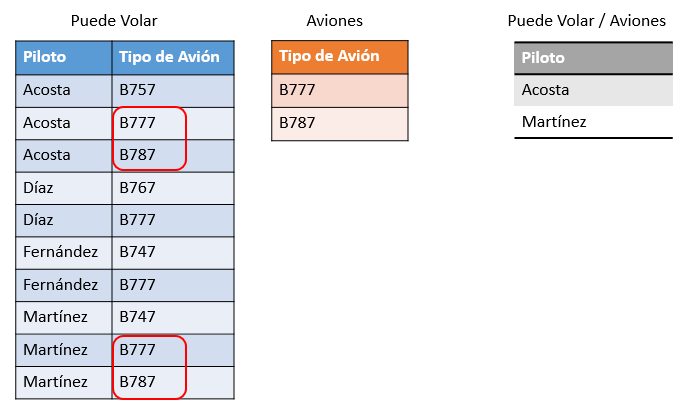
\includegraphics[scale=0.7]{division}
		\caption{División}
	\end{figure}

	\item \textbf{Asignación} ($r\leftarrow s$)

	$r$ no cambia al ejecutar operaciones de actualización sobre $s$.
\end{enumerate}

\subsection{Operadores extendidos}
\begin{enumerate}
	\item \textbf{Proyección generalizada}: permite operadores aritméticos como parte de una proyección.

	\[
		\pi_{F_{1},F_{2},\dots,F_{n}}(E)
	\]

	donde $E$ es una expresión de álgebra relacional, y $F_{i}$ es una expresión aritmética que involucra constantes y atributos del esquema $E$.

	\item \textbf{Funciones agregadas}: son funciones que toman como parámetro un multiconjunto%
	\footnote{Un \textbf{multiconjunto} es un conjunto en el que un valor puede aparecer muchas veces.}.
	\begin{lstlisting}
sum
count
min
max
avg
	\end{lstlisting}

	La forma general es: 
	\[
		_{G_{1},\dots G_{n}}\mathcal{G}_{F_{1}(A_{1}),\dots,F_{m}(A_{m})}(E)
	\]

	donde $E$ una expresión de álgebra relacional; $G_{i}$ es un atributo para formar grupos, $F_{i}$ es una función agregada, y $A_{i}$ es un atributo. Las tuplas de la relación resultado de $E$ se particionan en grupos de tal forma que
	\begin{enumerate}
		\item Todas las tuplas en un grupo tienen el mismo valor para $G_{i}\,\forall i\in[1,n]$
		\item Tuplas en distintos grupos tienen distinto valor para $G_{i}\,\forall i\in[1,n]$
	\end{enumerate}

	Para cada grupo, la relación tendrá una tupla $(g_{1},\dots,g_{n},a_{1},\dots,a_{m})$ donde para cada $i$, $a_{i}$ es el resultado de aplicar la función $F_{i}$ en el multiconjunto, para el atributo $A_{i}$ del grupo.

	\emph{Ejemplo: dada la relación EmpleadosPartTime(nombre,sucursal,salario), la siguiente expresión devuelve una relación con un solo atributo (sin nombre) y una sola fila, que contiene el valor de la suma de todos los salarios:} 
	\[
		\mathcal{G}_{sum(salario)}EmpleadosPartTime
	\]

	Se puede usar el operador \texttt{distinct} para eliminar múltiples ocurrencias de un valor.

	\emph{Ejemplo: con la misma relación anterior, la siguiente expresión devuelve una relación con un solo atributo (sin nombre) y una sola fila, que contiene la cantidad de sucursales:}
	\[
		\mathcal{G}_{count-distinct(sucursal)}EmpleadosPartTime
	\]

	Se puede usar el operador de \textbf{grupos}\textbf{\emph{ }}para particionar una relación y computar una función agregada a cada grupo.

	\emph{Ejemplo: con la misma relación anterior, la siguiente expresión devuelve una relación con dos atributos (sin nombres), que contiene la suma de salarios de cada sucursal:}
	\[
		_{sucursal}\mathcal{G}_{sum(salario)}EmpleadosPartTime
	\]

	\item \textbf{Join externo} (\emph{outer join}): es una extensión de la operación de \emph{join} que lidia con información faltante (\emph{null}s).
	\begin{enumerate}
		\item \emph{Left outer join} (\textbf{$r_{1}$$ $$\leftouterjoin\, r_{2}$}): hace un \emph{join} \emph{natural}, y toma todas las tuplas de $r_{1}$ que no matchearon con ninguna tupla de $r_{2}$, les agrega valores \emph{null} a los atributos de $r_{2}$, y los agrega al resultado.
		\item \emph{Right outer join} (\textbf{$r_{1}$ $\rightouterjoin\, r_{2}$}): hace un \emph{join} \emph{natural}, y toma todas las tuplas de $r_{2}$ que no matchearon con ninguna tupla de $r_{1}$, les agrega valores \emph{null} a los atributos de $r_{1}$, y los agrega al resultado.
		\item \emph{Full outer join} (\textbf{$r_{1}$ $\fullouterjoin\, r_{2}$}): combina las dos operaciones anteriores.
		\begin{figure}[H]
			\centering
			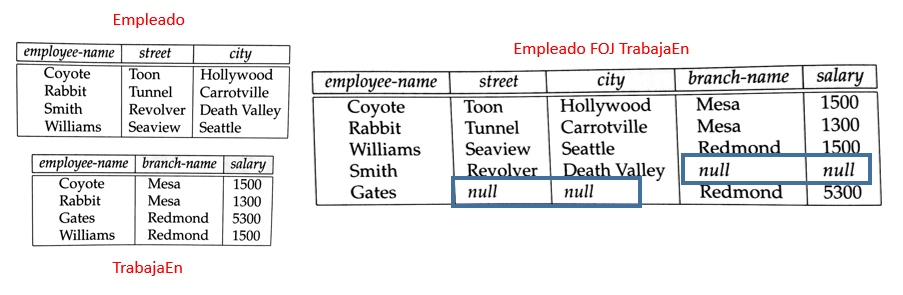
\includegraphics[scale=0.5]{fullouterjoin}
			\caption{Ejemplo de \emph{full outer join}}
		\end{figure}
	\end{enumerate}
\end{enumerate}

\subsection{Actualizaciones a bases de datos}
\subsubsection{Delete}
En álgebra relacional se expresa como $r\leftarrow r-E$, donde $r$ es una relación y $E$ es una expresión de consulta.

Solo se pueden borrar tuplas completas, no valores de atributos.

\subsubsection{Insert}
En álgebra relacional se expresa como $r\leftarrow r\cup E$, donde $r$ es una relación y $E$ es una expresión de consulta, o una relación constante con una sola tupla.

\subsubsection{Update}
En álgebra relacional se expresa como $r\leftarrow\pi_{F_{1},\dots,F_{n}}(r)$, donde $r$ es una relación y cada $F_{i}$ es, o el atributo i-ésimo de $r$, o una expresión que involucra solo constantes y el nuevo valor de $r$, que da el nuevo valor del atributo i-ésimo.

\subsection{Vistas (\emph{views})}
\textbf{Vista:} relación que no es parte del modelo lógico de la base de datos, pero que es visible para el usuario como una relación ``virtual''.

\begin{lstlisting}
CREATE VIEW v AS <expresion de consulta>
\end{lstlisting}

Limitaciones:
\begin{itemize}
	\item No se pueden ejecutar operaciones de \emph{update} sobre una vista, salvo que la vista sobre la relación $R$ cumpla lo siguiente:
	\begin{itemize}
		\item Deben usar \texttt{SELECT}, y no \texttt{SELECT DISTINCT}
		\item La cláusula \texttt{WHERE} no debe incluir a $R$ en una consulta anidada
		\item La cláusula \texttt{WHERE} no debe incluir a otra relación
		\item Los atributos del \texttt{SELECT} deben ser \texttt{NOT NULL}
	\end{itemize}

	El \emph{update} solo se ejecutará sobre los atributos del \texttt{SELECT}.

	\item A las operaciones de \emph{delete} sobre una vista se les pasa la cláusula \texttt{WHERE} de la vista (para borrar solo las tuplas que se pueden ver en la vista).

	\item Si las relaciones subyacentes son modificadas, la vista queda desactualizada. Por eso, en los motores, en una expresión que involucra una vista, la relación de la vista se recalcula al evaluar la expresión.
\end{itemize}

\textbf{Vista materializada:} vista que se evalúa y se almacena físicamente. Los cambios a estas vistas se realizan de forma \emph{incremental}(no se reconstruye toda la vista desde cero).

\section{Cálculo relacional}
COMPLETAR

\section{Lenguajes de consulta}
\textbf{Query:} expresión que solicita una porción de información.

Hay dos tipos de lenguajes de consulta (\emph{query languages}):
\begin{enumerate}
	\item \textbf{Procedurales:} el usuario indica una serie de operaciones a ejecutar sobre una base de datos para producir el resultado deseado. \emph{Ejemplos: SQL.}
	\item \textbf{No procedurales:} el usuario indica la información deseada, sin especificar el procedimiento para obtenerla. \emph{Ejemplos: Datalog (similar a Prolog).}
\end{enumerate}

\section{Integridad y seguridad}
En SQL, tenemos las siguientes restricciones:
\begin{itemize}
	\item \texttt{NOT NULL}: indica que un atributo no puede tener el valor \emph{null}
	\item \texttt{UNIQUE}: asegura que para todas las tuplas, el valor del atributo es único
	\item \texttt{PRIMARY KEY}: asegura que una o varias columnas tengan una identidad única, no nula
	\item \texttt{FOREIGN KEY}: asegura la integridad referencial de una tabla
	\item \texttt{CHECK}: asegura que el valor de un atributo satisface una condición especificada
	\item \texttt{DEFAULT}: especifica un valor por defecto cuando no se especifique ninguo
\end{itemize}

\subsection{Restricciones de dominio}
\begin{lstlisting}
CREATE DOMAIN color AS VARCHAR(10)
	DEFAULT 'SinColor'
	CHECK (value IN ('SinColor', 'Azul', 'Rojo'));

CAST relacion.Atributo AS <dominio>;

DROP DOMAIN <dominio>;

ALTER DOMAIN <dominio>;
\end{lstlisting}

\subsection{Restricciones de integridad referencial}
Ejemplo: 
\begin{lstlisting}
CREATE TABLE hospital (
	IdHosp SMALLINT,
	PRIMARY KEY (IdHosp));

CREATE TABLE medico (
	IdHosp SMALLINT,
	IdMedico SMALLINT,
	Nombre VARCHAR(40)
	PRIMARY KEY (IdMedico));

ALTER TABLE medico
	ADD CONSTRAINT FK_medico 
	FOREIGN KEY IdHosp 
	REFERENCES hospital(IdHosp);
\end{lstlisting}

\subsubsection{Acciones referenciales}
Son llamadas SQL que se ejecutan de forma automática ante la eliminación o actualización de una restricción de integridad referencial, para mantener la misma.

\begin{lstlisting}
ALTER TABLE medico 
	ADD CONSTRAINT FK_medico 
	FOREIGN KEY IdHosp 
	REFERENCES hospital(IdHosp)
		ON [DELETE|UPDATE] [SET DEFAULT|SET NULL|CASCADE|NO ACTION];
\end{lstlisting}

De esta forma, cuando se elimine o actualice una fila en la tabla \texttt{Hospital}, el sistema de base de datos ejecutará la acción especificada en la tabla \texttt{Medico}:
\begin{itemize}
	\item \texttt{SET DEFAULT / SET NULL}: se fija el valor predeterminado o nulo en la fila referenciante.
	\item \texttt{CASCADE}: al eliminar una tupla referenciada, las tuplas referenciantes son eliminadas. Al modificar la clave en la tabla referenciada, el correspondiente valor de la clave foránea es actualizado.
\end{itemize}

\subsection{Seguridad y autorizaciones}
Para brindar autorizaciones, se brindan privilegios. Los privilegios son tipos de autorizaciones para leer, insertar, actualizar o borrar datos. También existe el privilegio \texttt{references}, que permite declarar claves foráneas al crear relaciones nuevas.

Con la opción \texttt{WITH GRANT OPTION} se permite que el usuario que recibe el permiso se lo conceda a alguien más. El pase de autorizaciones de un usuario a otro se representa con un \textbf{grafo de autorización}, donde cada nodo es un usuario (la raíz es el DBA), y las aristas representan autorizaciones concedidas.

Un usuario tiene autorización sí y solo sí existe un camino desde la raíz del grafo hacia el nodo usuario.

\begin{lstlisting}
GRANT <privilegios>
	ON <[relacion|vista]>
	TO <[usuario|rol]>
	[WITH GRANT OPTION];
\end{lstlisting}

Para eliminar autorizaciones se usa el comando \texttt{REVOKE}. Por defecto, este comando tiene el efecto de revocar los privilegios que el usuario le brindó a otros. Para evitar este efecto cascada, se usa la opción \texttt{RESTRICT}.

\begin{lstlisting}
REVOKE <privilegios>
	ON <[relacion|vista]>
	FROM <[usuario|rol]>
	[RESTRICT];
\end{lstlisting}

Para crear roles:

\begin{lstlisting}
CREATE ROLE instructor;
\end{lstlisting}

\section{Triggers}
\textbf{Trigger:} comando que el sistema ejecuta automáticamente si un \emph{evento} satisface cierta \emph{condición}. Son un conjunto de acciones; por ejemplo, enviar un e-mail, ejecutar el \emph{rollback} de una transacción, o crear una copia de la base de datos.

\begin{lstlisting}
CREATE TRIGGER chequear_horario
[BEFORE|AFTER] [UPDATE|INSERT|DELETE] [OF atributo] ON curso
WHEN condicion
BEGIN
	acciones
END
\end{lstlisting}

\newpage
\part{Diseño de bases de datos}
Objetivos:
\begin{itemize}
	\item Reducir la redundancia de la información (porque ocupa espacio y es más difícil de actualizar): repetición de información en varias tuplas
	\item Eliminar las anomalías:
	\begin{itemize}
		\item De actualización: podría darse el caso de que actualizamos una tupla y no actualizamos otra tupla con el mismo dato
		\item De inserción: no es posible insertar ciertos datos sin insertar otros (posiblemente no relacionados)
		\item De eliminación: podría darse el caso de que eliminamos una tupla y, sin querer, borramos un dato importante
	\end{itemize}
	\item Devolver información rápidamente
\end{itemize}

Notación:
\begin{itemize}
	\item Nombre de esquemas: $R,S,R_{1},\dots,R_{n},S_{1},\dots,S_{n}$
	\item Instancias de esquemas: $r,s,r_{1},\dots r_{n},s_{1},\dots,s_{n}$
	\item Conjuntos de atributos: $\alpha,\beta,\gamma$
	\item Atributos: $A,B,C$
	\item Tuplas: $t_{1},t_{2}$
\end{itemize}

\section{Dependencias funcionales}
\begin{description}
	\item[Dependencia funcional] sea el esquema $R$, y sean $\alpha \subseteq R$ y $\beta\subseteq R$. La dependencia funcional $\alpha \to \beta$ se cumple si para cada par de tuplas $t_{1}, t_{2}$ tal que $t_{1}[\alpha] = t_{2}[\alpha]$, también se cumple que $t_{1}[\beta]=t_{2}[\beta]$. 

	Una dependencia funcional es \textbf{trivial} si $\beta\subseteq\alpha$. En particular, $\alpha\to\alpha$ es trivial.

	Un conjunto $K$ es superclave de $R$ si $K\to R$.

	Un conjunto $J$ es clave candidata de $R$ si $J\to R$ y además $\not\exists\gamma\subset J/\gamma\to R$.

	Una dependencia funcional, a diferencia de una diferencia multivaluada o de junta, prohíbe que ciertas tuplas existan.

	\item[Dependencias funcionales implicadas] sea el esquema $R$. Una dependencia funcional $f$ está lógicamente implicada por un conjunto de dependencias $F$, si para cada instancia de relación $r(R)$ que cumple $F$, también cumple $f$.
\end{description}

\subsection{Axiomas de Armstrong}
Se utilizan para hallar las dependencias funcionales implicadas, es
decir, $F^{+}$ de un conjunto $F$.
\begin{enumerate}
	\item Regla de reflexividad
	
	Si $\alpha$ es un conjunto de atributos y $\beta\subseteq\alpha,$ entonces $(\alpha\to\beta)\in F^{+}$

	\item Regla de augmentación

	Si $\alpha\to\beta$ es una dependencia funcional y $\gamma$ es un conjunto de atributos, entonces $(\gamma\alpha\to\gamma\beta)\in F^{+}$

	\item Regla de transitividad

	Si $\alpha\to\beta$ es una dependencia funcional y $\beta\to\gamma$ es otra dependencia funcional, entonces $(\alpha\to\gamma)\in F^{+}$
\end{enumerate}

Propiedades deducidas:
\begin{enumerate}
	\item Regla de unión

	Si se cumplen $\alpha\to\beta$ y $\alpha\to\gamma$, entonces también se cumple $\alpha\to\beta\gamma$

	\item Regla de descomposición

	Si se cumple $\alpha\to\beta\gamma$, entonces también se cumplen $\alpha\to\beta$ y $\alpha\to\gamma$

	\item Regla de pseudotransitividad

	Si se cumplen $\alpha\to\beta$ y $\gamma\beta\to\delta$, entonces también se cumple $\gamma\alpha\to\delta$
\end{enumerate}

\textbf{Teorema}: $R$ satisface la dependencia funcional $X\to Y$ sí y sólo sí $R$ descompone sin pérdida sobre los esquemas $XY$ y $X(R-XY)$, es decir, si $R$ satisface la dependencia de junta $*\left( XY, X(R-XY) \right)$

\subsection{Clausura y superclaves}
\textbf{Clausura de F:} sea $F$ un conjunto de dependencias funcionales sobre el esquema $R$. $F^{+}$ es el conjunto de dependencias funcionales implicadas por $F$.

\[
	F^{+}=\left\{ \alpha\to\beta/F\vDash\alpha\to\beta\right\} 
\]

\begin{algorithm}[H]
	Entrada: relación $R$, conjunto de dependencias funcionales $F$

	Salida: $F^{+}$
	\begin{enumerate}
		\item $F^{+}=F$

		\item Repetir hasta que $F^{+}$ no varíe:
		\begin{enumerate}
			\item Para cada dependencia funcional $f$ en $F^{+}$:

			Aplicar reglas de reflexividad y aumentación a $f$

			Agregar las dependencias funcionales restantes a $F^{+}$

			\item Para cada par de dependencias funcionales $f_{1},f_{2}$ en $F^{+}$:
			\begin{itemize}
				\item Si $f_{1},f_{2}$ pueden combinarse usando el axioma de transitividad:

				Agregar la dependencia funcional resultante a $F^{+}$
			\end{itemize}
		\end{enumerate}

		\item Devolver $F^{+}$
	\end{enumerate}
	\caption{Computar $F^{+}$}
\end{algorithm}

Para un esquema $R$ con $n$ atributos, hay $2^{n+1}$ posibles dependencias funcionales.

\textbf{Clausura de $\alpha$ bajo $F$}: es el conjunto de atributos de $R$ que dependen funcionalmente de $\alpha$.

\[
	\alpha_{F}^{+}=\left\{ \beta/\beta\subset R\,\wedge\, F\vDash\alpha\to\beta\right\} 
\]

\begin{algorithm}[H]
	Entrada: relación $R$, conjunto de dependencias funcionales $F$, atributo $\alpha$

	Salida: $\alpha_{F}^{+}$
	\begin{enumerate}
		\item $a^{+} = a$

		\item Repetir hasta que $a^{+}$ no varíe:
		\begin{enumerate}
			\item Para cada dependencia funcional $B\to Y\in F$:
			\begin{itemize}
				\item Si $B \subseteq a^{+}$: $a^{+} = a^{+}\cup Y$
			\end{itemize}
		\end{enumerate}
		
		\item Devolver $a^{+}$
	\end{enumerate}
	\caption{Computar $\alpha^{+}$}
\end{algorithm}

Usos del algoritmo de cálculo de la clausura de $a^{+}$:
\begin{enumerate}
	\item Para determinar si $\alpha$ es una superclave de $R$: debe cumplirse que $\alpha^{+}=R$.
	\item Para determinar si la dependencia funcional $\alpha\to\beta\in F^{+}$: debe cumplirse que $\beta\subseteq\alpha^{+}$.
	\item Es una forma alternativa de calcular $F^{+}$
\end{enumerate}

\begin{algorithm}[H]
	Entrada: relación $R$, conjunto de dependencias funcionales $F$

	Salida: claves candidatas de $R$
	\begin{enumerate}
		\item Dibujar el grafo de dependencias funcionales (si $X\to Y\in F$, dibujar una arista entre $X$ e $Y$)
		\item $V_{ni}=$ atributos sin aristas entrantes
		\item $V_{oi}=$ atributos que solo tienen aristas entrantes
		\item $K=\{\}$
		\item Repetir hasta que no se pueda agregar nada a $K$:
		\begin{enumerate}
			\item $CC=$ todos los atributos de $V_{ni}$
			\item Agregar a $CC$ un atributo de $R$ que no esté en $V_{oi}$ ni $V_{ni}$
			\item $K=K\cup CC$
		\end{enumerate}
		\item Devolver $K$
	\end{enumerate}
	\caption{Cálculo de claves candidatas mediante un grafo}
\end{algorithm}

\subsection{Cubrimiento minimal}
\begin{description}
	\item[Atributo extráneo:] atributo de una dependencia funcional que se puede quitar de la misma sin cambiar\emph{ }la clausura del conjunto de dependencias funcionales. 

	Sea el conjunto de dependencias funcionales $F$ y la dependencia funcional $\alpha\to\beta$ en $F$.
	\begin{itemize}
		\item El atributo $A$ es extráneo en $\alpha$ si, cuando lo sacamos de $\alpha$, la dependencia funcional se sigue cumpliendo ($B\in(\alpha-A)_{F}^{+}$). Formalmente:
		\begin{itemize}
			\item $A\in\alpha$, y
			\item $F$ implica lógicamente a $\left(F-\left\{ \alpha\to B\right\} \right)\cup\left\{ \left(\alpha-A\right)\to\beta\right\} $
		\end{itemize}

		\item El atributo $B$ es extráneo en $\beta$ si, cuando lo sacamos de $\beta$, la dependencia funcional se sigue cumpliendo ($\alpha\to(\beta-B)$) Formalmente:
		\begin{itemize}
			\item $B\in\beta$, y
			\item El conjunto $\left(F-\left\{ \alpha\to\beta\right\} \right)\cup\left\{ \alpha\to\left(\beta-B\right)\right\}$ implica lógicamente a $F$
		\end{itemize}
	\end{itemize}

	\item[Cubrimiento minimal:] El cubrimiento minimal $F_{min}$ para $F$ es un conjunto de dependencias funcionales tales que $F$ implica todas las dependencias en $F_{min}$, y $F_{min}$ implica todas las
dependencias en $F$.

	$F_{min}$ debe tener las propiedades siguientes:
	\begin{itemize}
		\item Ninguna dependencia funcional en $F_{min}$ contiene un atributo extráneo
		\item No existen dos dependencias funcionales $\alpha_{1}\to\beta$ y $\alpha_{2}\to\gamma$ en $F_{min}$ tales que $\alpha_{1}=\alpha_{2}$. Es decir, los lados izquierdos deben ser únicos
	\end{itemize}
\end{description}

\begin{algorithm}[H]
	Entrada: conjunto de dependencias funcionales $F$

	Salida: cubrimiento minimal $F_{min}$
	\begin{enumerate}
		\item Usar el axioma de la descomposición para dejar un solo atributo en el lado derecho de cada dependencia funcional.

		\item Eliminar los atributos extráneos de los lados izquierdos.

		Sea $Y\to B$ una dependencia funcional en $F$, con al menos dos atributos en $Y$. Sea $Z$ igual a $Y$ pero con algún atributo de menos. Si $F$ implica a $Z\to B$, entonces reemplazar $Y\to B$ con $Z\to B$.

		\item Eliminar las dependencias funcionales redundantes (es decir, que se deducen de los axiomas de Armstrong).
	\end{enumerate}
	\caption{Cálculo de cubrimiento minimal}
\end{algorithm}

\emph{Ejemplo: sea el conjunto de dependencias $F=\{A\to BD,B\to CD,AC\to E\}$. Calcular el cubrimiento minimal.}
\begin{enumerate}
	\item \emph{Dejar todos los lados derechos con un único atributo.}
	
	\emph{$F_{min}=\{A\to B,A\to D,B\to C,B\to D,AC\to E\}$}

	\item \emph{Eliminar todos los atributos redundantes del lado izquierdo.}
	\begin{enumerate}
		\item \emph{Hay que analizar solamente la dependencia que tiene lado izquierdo compuesto: $AC\to E$.}
		\item \emph{¿$C$ es redundante en $AC\to E$? Hay que verificar si $E$ está en $A_{F}^{+}$. Como $A_{F}^{+}=ABCDE$, entonces $C$ es redundante en $AC\to E$ y podemos reemplazar esta dependencia funcional por
$A\to E$.}
	\end{enumerate}

	\emph{$F_{min}=\{A\to B,A\to D,B\to C,B\to D,A\to E\}$}

	\item \emph{Eliminar las dependencias redundantes.}
	\begin{itemize}
		\item \emph{Hay que revisar una por una todas las dependencias de $F_{min}$. En caso de que una sea redundante, se la elimina de $F_{min}$ y se sigue analizando el resto tomando como referencia el nuevo $F_{min}$. }
		\item \emph{¿$A\to D$ es redundante en $F_{c}$? Hay que verificar si $D$ está en $A_{F_{c}-\{A\to D\}}^{+}$}
		\begin{itemize}
			\item \emph{$F_{min}-\{A\to D\}=\{A\to B,B\to C,B\to D,A\to E\}$}
			\item \emph{$A_{F_{min}-\{A\to D\}}^{+}=ABCDE$}
			\item \emph{Como $D\in F_{min}-\{A\to D\}$, $A\to D$ es redundante}
		\end{itemize}

		$F_{min}=\left\{ A\to B,B\to C,B\to D,A\to E\right\} $
	\end{itemize}

	Puede comprobarse que el resto de las dependencias funcionales no es redundante.
\end{enumerate}

\section{Primera forma normal (1FN)}
\textbf{Dominio atómico:} los elementos del dominio se consideran unidades indivisibles.

Una relación con esquema $R$ está en 1FN si los dominios de sus atributos son atómicos, y si no hay atributos similares repetidos.

\textbf{\emph{Ejemplo}}: la siguiente relación no está en 1FN.\\

\begin{center}
	\begin{tabular}{|c|c|c|c|}
		\hline 
		\uline{Título Libro} & Autor 1 & Autor 2 & Autor 3\\
		\hline 
		\hline 
		Database System Concepts & Avi Silberschatz & Henry Korth & S. Sudarshan\\
		\hline 
		Applied Cryptography & Bruce Schneier & NULL & NULL\\
		\hline 
	\end{tabular}
\end{center}

~\\

Para normalizarla, hay que dividirla en dos relaciones.\\

\begin{minipage}{0.5\textwidth}
	\begin{center}
		\begin{tabular}{|c|c|}
			\hline 
			\uline{ID libro} & Título Libro\\
			\hline 
			\hline 
			1 & Database System Concepts\\
			\hline 
			2 & Applied Cryptography\\
			\hline 
		\end{tabular}
	\end{center}
\end{minipage}
\begin{minipage}{0.45\textwidth}
	\begin{center}
		\begin{tabular}{|c|c|}
			\hline 
			\uline{ID libro} & \uline{Autor}\\
			\hline 
			\hline 
			1 & Avi Silberschatz\\
			\hline 
			1 & Henry Korth\\
			\hline 
			1 & S. Sudarshan\\
			\hline 
			2 & Bruce Schneier\\
			\hline 
		\end{tabular}
	\end{center}
\end{minipage}

\section{Descomposición de una relación}
Sea el esquema relacional $R$. El conjunto de esquemas $\left\{ R_{1},R_{2},\dots,R_{n}\right\}$ es una descomposición de $R$ si
\[
	R = R_{1}\cup R_{2}\cup\dots\cup R_{n}
\]

Sea la relación $r(R)$. Sean $r_{i}=\pi_{R_{i}}(r)$ para $i=1,2,\dots,n$. Es decir, $\left\{ r_{1},r_{2},\dots,r_{n}\right\} $ es la base de datos que resulta de descomponer $R$ en $\left\{ R_{1},R_{2},\dots,R_{n}\right\} $. Siempre se verifica que
\[
	r\subseteq r_{1}\bowtie r_{2}\bowtie\dots\bowtie r_{n}
\]

Es decir, $r$ es un subconjunto de la junta de la descomposición (la junta podría tener tuplas que no están en $r$).

Propiedades deseadas de la descomposición:
\begin{enumerate}
	\item \textbf{Sin pérdida de información}
	
	Verifica que \textbf{\emph{$r=\pi_{R_{1}}(r)\bowtie\pi_{R_{2}}(r)\bowtie\dots\bowtie\pi_{R_{n}}(r)$.}}

	\item \textbf{Preservación de dependencias}

	Una descomposición que verifica que $F'^{+}=F^{+}$ preserva dependencias, donde $F' = F_{1} \cup F_{2} \cup \dots \cup F_{n}$ son las dependencias proyectadas.

	Esta propiedad es deseable porque significa que podemos chequear si se cumple la dependencia con solo verificarla en una relación individual, y no necesitamos hacer un \emph{join} de las relaciones de la descomposición.

	\item \textbf{Poca o nula redundancia de información}
\end{enumerate}

\begin{algorithm}[H]
	Entrada: relación $R$, relación $R_{i}$, conjunto de dependencias funcionales $F$

	Salida: conjunto de dependencias funcionales que se verifican en $R_{i}$ ($F_{i}$)
	\begin{enumerate}
		\item $F_{i}=\{\}$
		\item Para cada conjunto de atributos $X$ que es un subconjunto de atributos de $R_{i}$:
		\begin{enumerate}
			\item Calcular $X_{F}^{+}$
			\item $F_{i}=F_{i}\cup\left\{ X\to A\right\} $, tal que $A\subseteq X_{F}^{+}$ y $A\subseteq R_{i}$
		\end{enumerate}
		\item Devolver $F_{i}$
	\end{enumerate}
	\caption{Cálculo de la proyección de dependencias $F_{i}$}
\end{algorithm}

\begin{algorithm}[H]
	Entrada: dependencia funcional $A\to B$, conjunto de dependencias funcionales $F$, descomposición $\left\{ R_{1},\ldots,R_{n}\right\}$

	Salida: ``verdadero'' si la descomposición preserva $A\to B$
	\begin{enumerate}
		\item $Z=A$
		\item Repetir hasta que $Z$ no varíe o hasta que $Z$ incluya a $B$:
		\begin{itemize}
			\item Para cada $R_{i}$: $Z=Z\cup\left[\left(Z\cap R_{i}\right)^{+}\cap R_{i}\right]$
		\end{itemize}
		\item Si $B\subseteq Z$: devolver ``verdadero''
		\item Si no: devolver ``falso''.
	\end{enumerate}
	\caption{Cálculo para saber si una descomposición preserva una dependencia}
\end{algorithm}

\subsection{Descomposición SPI en 2 relaciones}
Sea el esquema relacional $R$, y sea $F$ el conjunto de dependencias funcionales sobre $R$. Sean $R_{1}$ y $R_{2}$ una descomposición de $R$. Esta descomposición es \emph{sin pérdida de información} (SPI) si al menos una de las siguientes dependencias funcionales está en $F^{+}$:
\begin{itemize}
	\item $R_{1}\cap R_{2}\to R_{1}-R_{2}$
	\item $R_{1}\cap R_{2}\to R_{2}-R_{1}$
\end{itemize}

\emph{Ejemplo: ¿La descomposición de $R(A,B,C,D,E,F)$ en $R_{1}=(A,D,E,F)$ y $R_{2}=(B,C,D)$ es SPI respecto de $F=\{A\to BD,B\to CD,AC\to E\}$?}
\begin{itemize}
	\item $R_{1}\cap R_{2}=D$
	\item $R_{1}-R_{2}=AEF$
	\item $R_{2}-R_{1}=BC$
	\item \emph{Como $D_{F}^{+}=\{D\}$, vemos que no se cumplen ni $R_{1}\cap R_{2}\to R_{1}-R_{2}$ ni $R_{1}\cap R_{2}\to R_{2}-R_{1}$. Por lo tanto, esta descomposición no es SPI.}
\end{itemize}

\subsection{Descomposición SPI en más de 2 relaciones}

El algoritmo \textbf{Chase Tableau} se utiliza para verificar si una descomposición de $R$ en $R_{1},\ldots,R_{k}$ ($k>2)$ es SPI. Es decir, si la proyección de un esquema restringido por dependencias en una descomposición, puede recuperarse haciendo el \emph{join} de las proyecciones.

\begin{algorithm}[H]
	Entrada: esquema de relación $R$, conjunto de dependencias funcionales $F$, descomposición $\left\{ R_{1},\ldots,R_{k}\right\}$

	Salida: ``verdadero'' si $\left\{ R_{1},\ldots,R_{n}\right\} $ descompone SPI.
	\begin{enumerate}
		\item Armar una matriz $T^{(0)}$ con las relaciones $R_{i}$ en las filas ($i=1,\ldots,k$) y los atributos $A_{j}$ en las columnas. Cada elemento de la matriz tendrá valor:
\[
	m_{ij}=
	\begin{cases}
		a_{j} & \text{ si }A_{j}\in R_{i}\text{ (variable distinguida)}\\
		b_{ij} & \text{ si }A_{j}\not\in R_{i}\text{ (variable ligada)}
	\end{cases}
\]

		\item $i=1$

		\item Obtener $T^{(i)}$:
		\begin{itemize}
			\item Para cada dependencia funcional $X\to Y\in F$:
			\begin{itemize}
				\item Si $\exists$ tuplas $t_{1},t_{2}$ tal que $t_{1}[X]=t_{2}[x]$, realizar un cambio de variable en $t_{1}[Y]$ y en $t_{2}[Y]$
				\begin{itemize}
					\item Variables ligadas por distinguidas
					\item Si hay dos ligadas, poner la de menor subíndice
				\end{itemize}
			\end{itemize}
		\end{itemize}

		\item Si hay una fila sólo con variables distinguidas, devolver ``verdadero''.

		\item Si $T^{(i)}=T^{(i-1)}$ y además no hay una fila sólo con variables distinguidas, devolver ``falso''.
		
		\item Si no, $i\leftarrow i+1$ y volver a 3.
	\end{enumerate}
	\caption{Algoritmo Chase Tableau}
\end{algorithm}

\emph{Ejemplo: sea el esquema de relación $R(A,B,C,D)$ con $F=\{A\to B,B\to C,CD\to A\}$. Sea la descomposición $R_{1}=(A,D)$, $R_{2}=(A,C)$, $R_{3}=(B,C,D)$. ¿La descomposición es SPI?}

\begin{center}
	\begin{tabular}{|c|c|c|c|c|}
		\hline 
		 & $A$ & $B$ & $C$ & $D$\\
		\hline 
		\hline 
		$R_{1}(A,D)$ & \textbf{$a_{1}$} & \textbf{$b_{12}$} & $b_{13}$ & $a_{4}$\\
		\hline 
		$R_{2}(A,C)$ & $a_{1}$ & $b_{22}$ & $a_{3}$ & $b_{24}$\\
		\hline 
		$R_{3}(B,C,D)$ & $b_{31}$ & $a_{2}$ & $a_{3}$ & \textbf{$a_{4}$}\\
		\hline 
	\end{tabular}
\end{center}

Aplicamos $A\to B$. Como $a_{1}$ es igual en las primeras dos filas, pero $b_{12}$ y $b_{22}$ no, cambiamos $b_{22}$ por $b_{12}$ en la segunda fila.

\begin{center}
	\begin{tabular}{|c|c|c|c|c|}
		\hline 
		 & $A$ & $B$ & $C$ & $D$\\
		\hline 
		\hline 
		$R_{1}(A,D)$ & $a_{1}$ & $b_{12}$ & $b_{13}$ & $a_{4}$\\
		\hline 
		$R_{2}(A,C)$ & $a_{1}$ & $\mathbf{b_{12}}$ & $a_{3}$ & $b_{24}$\\
		\hline 
		$R_{3}(B,C,D)$ & $b_{31}$ & $a_{2}$ & $a_{3}$ & \textbf{$a_{4}$}\\
		\hline 
	\end{tabular}
\end{center}

Aplicamos $B\to C.$ Las filas 1 y 2 coinciden en $b_{12}$ pero no en $c$. Entonces, cambiamos $b_{13}$ por $a_{3}$ en la fila 1.

\begin{center}
	\begin{tabular}{|c|c|c|c|c|}
		\hline 
		 & $A$ & $B$ & $C$ & $D$\\
		\hline 
		\hline 
		$R_{1}(A,D)$ & $a_{1}$ & $b_{12}$ & $\mathbf{a_{3}}$ & $a_{4}$\\
		\hline 
		$R_{2}(A,C)$ & $a_{1}$ & $b_{12}$ & $a_{3}$ & $b_{24}$\\
		\hline 
		$R_{3}(B,C,D)$ & $b_{31}$ & $a_{2}$ & $a_{3}$ & \textbf{$a_{4}$}\\
		\hline 
	\end{tabular}
\end{center}

Aplicamos $CD\to A$. Las filas 1 y 3 tienen mismo valor para $c$ y $d$, pero distinto valor para $a$. Por lo tanto, cambiamos $b_{31}$ por $a_{1}$ en la tercera fila.

\begin{center}
	\begin{tabular}{|c|c|c|c|c|}
		\hline 
		 & $A$ & $B$ & $C$ & $D$\\
		\hline 
		\hline 
		$R_{1}(A,D)$ & $a_{1}$ & $b_{12}$ & $a_{3}$ & $a_{4}$\\
		\hline 
		$R_{2}(A,C)$ & $a_{1}$ & $b_{12}$ & $a_{3}$ & $b_{24}$\\
		\hline 
		$R_{3}(B,C,D)$ & $\mathbf{a_{1}}$ & $a_{2}$ & $a_{3}$ & \textbf{$a_{4}$}\\
		\hline 
	\end{tabular}
\end{center}

En este punto notamos que la fila 3 tiene valores de la forma $a_{j}$. Como son todas variables distinguidas, la descomposición es sin pérdida de información.

\section{Segunda forma normal (2FN)}
\textbf{Atributo primo:} atributo de $R$ que pertenece a una clave candidata.

Sea $R$ una relación y $F$ el conjunto de sus dependencias funcionales. $R$ estará en 2FN si para toda dependencia funcional $X\to Y$ que está en en $F^{+}$, se cumple al menos una de las siguientes condiciones:
\begin{enumerate}
	\item $X\to Y$ es trivial
	\item $Y$ es un atributo primo,
	\item $X$ no es un subconjunto de una clave candidata
\end{enumerate}

\textbf{\emph{Ejemplo:}} la siguiente relación no está en 2FN porque \emph{Dirección de local} depende sólo de \emph{ID de local}, que no es una clave.

\begin{center}
	\begin{tabular}{|c|c|c|}
		\hline 
		\uline{ID de cliente} & \uline{ID de local} & Dirección de local\\
		\hline 
		\hline 
		1 & 1 & Los Angeles\\
		\hline 
		1 & 3 & San Francisco\\
		\hline 
		2 & 1 & Los Angeles\\
		\hline 
	\end{tabular}
\end{center}

$F=\{Id\, cliente,Id\, local\to Direccion\, local;Id\, local\to Direccion\, local\}$.

\emph{La segunda dependencia funcional no es trivial, el lado derecho no pertenece a una clave candidata, y el lado izquierdo es un subconjunto de la clave candidata.}

\emph{Para normalizarla, hay que dividirla en dos relaciones.}\\

\begin{minipage}{0.5\textwidth}
	\begin{center}
		\begin{tabular}{|c|c|}
			\hline 
			\uline{ID de cliente} & \uline{ID de local}\\
			\hline 
			\hline 
			1 & 1\\
			\hline 
			1 & 3\\
			\hline 
			2 & 1\\
			\hline 
		\end{tabular}
	\end{center}
\end{minipage}
\begin{minipage}{0.5\textwidth}
	\begin{center}
		\begin{tabular}{|c|c|}
			\hline 
			\uline{ID de local} & Dirección de local\\
			\hline 
			\hline 
			1 & Los Angeles\\
			\hline 
			3 & San Francisco\\
			\hline 
		\end{tabular}
	\end{center}
\end{minipage}

\section{Forma Normal Boyce-Codd (FNBC)}
Un esquema de relación $R$ está en FNBC con respecto a un conjunto de dependencias funcionales $F$ si, para todas las dependencias funcionales en $F^{+}$ de la forma $\alpha\to\beta$, donde $\alpha\subseteq R$ y $\beta\subseteq R$, se cumple alguna de las siguientes:
\begin{itemize}
	\item $\alpha\to\beta$ es trivial (es decir, $\beta\subseteq\alpha$)
	\item $\alpha$ es una superclave para $R$ 
\end{itemize}

Propiedades:
\begin{itemize}
	\item Cualquier relación de dos atributos está en FNBC
	\item Brinda eliminación de anomalías
	\item Brinda una descomposición SPI
	\item No garantiza que se preserven las dependencias funcionales
\end{itemize}

Para verificar si una dependencia funcional $\alpha\to\beta$ viola FNBC, alcanza con computar $\alpha^{+}$ y ver si es $R$.

Para verificar si una relación $R$ está en FNBC, alcanza con ver si las dependencias de $F$ no violan FNBC.

Para verificar si una descomposición $R_{i}$ está en FNBC, para cada subconjunto $\alpha$ de atributos de $R_{i}$, verificar que $\alpha_{F}^{+}$ o no incluya atributos de $R_{i}-\alpha$, o incluya todos los atributos de $R_{i}$.

\begin{algorithm}[H]
	Entrada: una relación $R$, un conjunto de dependencias funcionales $F$

	Salida: una descomposición $\rho=\left\{ R_{1},\ldots,R_{n}\right\}$ tal que $R_{i}$ está en FNBC con respecto a $F_{i}$
	\begin{enumerate}
		\item $\rho=R$
		\item Repetir hasta que no haya esquemas en $\rho$ que violen FNBC
		\begin{enumerate}
			\item Elegir una dependencia funcional $X\to Y$ que viole FNBC sobre $\rho_{i}$
			\item Descomponer $\rho_{i}$ en dos relaciones:
			\begin{itemize}
				\item $R_{1}(XY)$
				\item $R_{2}(X(R-XY))$
			\end{itemize}
			\item En $\rho$, reemplazar $\rho_{i}$ por $R_{1}$ y $R_{2}$
		\end{enumerate}
	\item Devolver $\rho$
	\end{enumerate}
	\caption{Descomposición FNBC}
\end{algorithm}

\section{Tercera forma normal (3FN)}
\begin{quote}
	\emph{A statement of Codd's definition of 3NF, paralleling the traditional pledge to give true evidence in a court of law, was given by Bill Kent: [Every] non-key [attribute] must provide a fact about the key, the whole key, and nothing but the key. A common variation supplements this definition with the oath: so help me Codd.}

	\emph{Requiring existence of the key ensures that the table is in 1NF; requiring that non-key attributes be dependent on the whole key ensures 2NF; further requiring that non-key attributes be dependent on nothing but the key ensures 3NF.}
\end{quote}

Un esquema de relación $R$ está en 3FN con respecto a un conjunto de dependencias funcionales $F$ si, para todas las dependencias funcionales en $F^{+}$ de la forma $\alpha \to \beta$, donde $\alpha \subseteq R$ y $\beta \subseteq R$, se cumple alguna de las siguientes:
\begin{itemize}
	\item $\alpha\to\beta$ es trivial (es decir, $\beta\subseteq\alpha$)
	\item $\alpha$ es una superclave para $R$ 
	\item $\beta$ es un atributo primo
\end{itemize}

Dicho de otra forma, $R$ no debe tener dependencias funcionales transitivas: todos los atributos que no son clave deben depender funcionalmente de la clave primaria.

Propiedades:
\begin{itemize}
	\item No tiene pérdida de información
	\item No hay pérdida de dependencias
	\item No garantiza la eliminación de anomalías (es decir, tiene redundancia)
	\item Es menos estricta que FNBC (FNBC $\implies$3FN)
\end{itemize}

\begin{algorithm}[H]
	Entrada: una relación $R$, un cubrimiento minimal $F_{min}$

	Salida: una descomposición $\rho=\left\{ R_{1},\ldots,R_{n}\right\}$ tal que $R_{i}$ está en 3FN con respecto a $F_{i}$
	\begin{enumerate}
		\item $\rho=\{\}$
		\item Para cada dependencia funcional $X\to Y\in F_{min}$:
			
		$\rho=\rho\cup R_{i}\left(XY\right)$

		\item Si existen $R_{i},R_{j}\in\rho$ tal que $R_{i}\subseteq R_{j}$:

		$\rho=\rho-R_{i}$

		\item Si ninguna relación es una superclave de $R$, y $K$ es una clave para $R$

		$\rho=\rho\cup K$

		\item Devolver $\rho$\protect\caption{Descomposición 3FN}
	\end{enumerate}
\end{algorithm}

\textbf{\emph{Ejemplo:}} la siguiente relación no está en 3FN porque \emph{Fecha de nacimiento del ganador} depende sólo de \emph{Ganador}, que depende de la clave candidata \emph{\{Torneo, Año\}}.

\begin{center}
	\begin{tabular}{|c|c|c|c|}
		\hline 
		\uline{Torneo} & \uline{Año} & Ganador & Fecha de nacimiento de ganador\\
		\hline 
		\hline 
		Indiana Invitational  & 1998 & Al Fredrickson  & 21 Julio 1975\\
		\hline 
		Cleveland Open  & 1999 & Bob Albertson  & 28 Septiembre 1968\\
		\hline 
		Des Moines Masters  & 1999 & Al Fredrickson  & 21 Julio 1975\\
		\hline 
		Indiana Invitational  & 1999 & Chip Masterson  & 14 Marzo 1977\\
		\hline 
	\end{tabular}
\end{center}

$F=\{Torneo,A\tilde{n}o\to Ganador,Ganador\to Fecha\, nacimiento\, ganador\}$. La segunda dependencia funcional no es trivial, el lado derecho no pertenece a una clave candidata (no es atributo primo), y el lado izquierdo no es una superclave.

Para normalizarla, hay que dividirla en dos relaciones.\\

\begin{minipage}{0.5\textwidth}
	\begin{center}
		\begin{tabular}{|c|c|c|}
			\hline 
			\uline{Torneo} & \uline{Año} & Ganador\\
			\hline 
			\hline 
			Indiana Invitational  & 1998 & Al Fredrickson \\
			\hline 
			Cleveland Open  & 1999 & Bob Albertson \\
			\hline 
			Des Moines Masters  & 1999 & Al Fredrickson \\
			\hline 
			Indiana Invitational  & 1999 & Chip Masterson \\
			\hline 
		\end{tabular}
	\end{center}
\end{minipage}
\begin{minipage}{0.5\textwidth}
	\begin{center}
		\begin{tabular}{|c|c|}
			\hline 
			\uline{Ganador} & Fecha de nacimiento\\
			\hline 
			\hline 
			Chip Masterson  & 14 Marzo 1977\\
			\hline 
			Al Fredrickson  & 21 Julio 1975\\
			\hline 
			Bob Albertson  & 28 Septiembre 1968\\
			\hline 
		\end{tabular}
	\end{center}
\end{minipage}

\section{Dependencias multivaluadas}
Una dependencia multivaluada expresa que dos conjuntos de atributos en un esquema son mutuamente independientes.

Sean los conjuntos de atributos \emph{disjuntos} $A$ y $B$ de la relación $R(A,B,U-A-B)$. Sean las tuplas $t_{1}$ y $t_{2}$. La dependencia multivaluada $A\twoheadrightarrow B$ indica que si $t_{1}[A]=t_{2}[A]$, entonces podemos encontrar tuplas $t_{3}$ y $t_{4}$ tales que:
\begin{itemize}
	\item $t_{1}[A]=t_{2}[A]=t_{3}[A]=t_{4}[A]$
	\item $t_{3}[B]=t_{1}[B]$
	\item $t_{3}[U-A-B]=t_{2}[U-A-B]$
	\item $t_{4}[B]=t_{2}[B]$
	\item $t_{4}[U-A-B]=t_{1}[U-A-B]$
\end{itemize}

\begin{figure}[H]
	\centering
	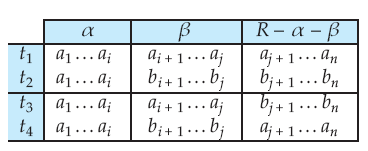
\includegraphics[scale=0.8]{multivalued_dependency}
	\caption{Dependencia multivaluada $\alpha \twoheadrightarrow \beta$}
\end{figure}

\textbf{\emph{Ejemplo:}} \emph{sea $R(curso, libro, profesor)$ una relación que indica una lista de cursos universitarios, los libros que se usan en el curso, y los profesores que la dictan.}

\begin{center}
	\begin{tabular}{|c|c|c|}
		\hline 
		\emph{Curso} & \emph{Libro} & \emph{Profesor}\\
		\hline 
		\hline 
		Álgebra II & David Lay - Algebra Lineal & Acero\\
		\hline 
		Álgebra II & Strang - Algebra Lineal & Acero\\
		\hline 
		Álgebra II & David Lay - Algebra Lineal & Piortrowsky\\
		\hline 
		Algebra II & Strang - Algebra Lineal & Piortrowsky\\
		\hline 
	\end{tabular}
\end{center}

\emph{Dado que los profesores de un curso y los libros de un curso son independientes entre sí, esta relación tiene una DMV. Si tuviésemos que agregar un nuevo libro al curso ``Álgebra II'', deberíamos agregar una tupla para cada profesor del curso. Es decir, formalmente, hay dos DMV en esta relación: $\{curso\} \twoheadrightarrow \{libro\}$
y $\{curso\} \twoheadrightarrow \{profesor\}$. Esta relación exhibe redundancia.}\\

\textbf{Dependencia multivaluada:} no existen en el esquema original pero son satisfechas por la descomposición del mismo.

\subsection{Propiedades de las DMVs}
\begin{itemize}
	\item $\alpha\twoheadrightarrow\beta$ es \textbf{trivial} si $\beta\subseteq\alpha$ ó si $R=\alpha\beta$.
	\item Una dependencia multivaluada garantiza que ciertas tuplas existan.
	\item \textbf{Regla de transitividad} \textbf{multivaluada}: Si $\alpha\twoheadrightarrow\beta$ y $\beta\twoheadrightarrow c$, entonces $\alpha\twoheadrightarrow c-\beta$
	\item \textbf{Regla de replicación}: si $\alpha\to\beta$, entonces $\alpha\twoheadrightarrow\beta$. La inversa \textbf{no} es cierta.
	\item \textbf{Regla de interacción} \footnote{Esta regla puede agregar dependencias funcionales a $M$}: si 			$\begin{cases}
		\alpha\twoheadrightarrow\beta\\
		\gamma\to Z
	\end{cases}$ y existe un $\gamma$ tal que
	$\begin{cases}
		Z\subseteq\beta\\
		\gamma\cap\beta=\emptyset
	\end{cases}$, entonces $\alpha\to Z$
	\item \textbf{Regla de aumentación}: si $\alpha\twoheadrightarrow\beta$ entonces $\alpha w\twoheadrightarrow\beta$.
	\item \textbf{Regla del complemento}: si $\alpha\twoheadrightarrow\beta$, entonces $\alpha\twoheadrightarrow R-\alpha\beta$
	\item \textbf{Regla de unión}: si $\alpha\twoheadrightarrow\beta$, y $\alpha\twoheadrightarrow c$, entonces $\alpha\twoheadrightarrow\beta c$
	\item \textbf{Regla de descomposición}: si $\alpha\twoheadrightarrow\beta$, y $\alpha\twoheadrightarrow c$, entonces 
	$\begin{cases}
		\alpha\twoheadrightarrow\beta-c\\
		\alpha\twoheadrightarrow c-\beta\\
		\alpha\twoheadrightarrow\beta\cap c
	\end{cases}$
	\item \textbf{Regla de pseudotransitividad:} si $\alpha\twoheadrightarrow\beta$ y $\beta c\twoheadrightarrow\gamma$, entonces $\alpha c\twoheadrightarrow\gamma-\beta c$
	\item Si $R=\left\{ A_{1},\ldots,A_{n},B_{1},\ldots,B_{m}\right\} $, entonces $\left\{ A_{1}, \ldots, A_{n} \right\} \twoheadrightarrow \left\{ B_{1}, \ldots, B_{m} \right\}$
\end{itemize}

\textbf{Teorema}: las únicas DMVs implicadas por un conjunto de DFs son de la forma $X \twoheadrightarrow Y$, donde $Y \subseteq X^{+}$ o $R - XY \subseteq X^{+}$.

\textbf{Teorema}: las únicas DFs implicadas por un conjunto de DMVs son las triviales.

\textbf{Teorema}: un conjunto de DFs de tipo $x_{i} \to y_{i}$ sólo implica DMVs de tipo $x_{i} \twoheadrightarrow y_{i}$.

\textbf{Teorema}: sea $r$ una instancia del esquema de relación $R$, $X, Y$ subconjuntos de $R$, y $Z = R - XY$. La relación $r$ satisface la DMV $X \twoheadrightarrow Y$ sí y solo sí $R_{1} = XY$ y $R_{2} = X \cup Z$ descomponen sin pérdida de información a $r$.

\begin{algorithm}[H]
	Entrada: relación $r(R)$

	Salida: ``verdadero'' si la dependencia multivaluada $X \twoheadrightarrow Y$ se satisface
	\begin{enumerate}
		\item Proyectar $r$ en $R_{1}(XY)$ y $R_{2}(X,R-XY)$
		\item Calcular $R_{1}\bowtie R_{2}$
		\item Si $r=R_{1}\bowtie R_{2}$ devolver ``verdadero''
	\end{enumerate}
	\caption{Verificar si $r$ satisface la dependencia multivaluada $X\twoheadrightarrow Y$}
\end{algorithm}

\begin{algorithm}[H]
	Entrada: conjunto de dependencias funcionales y multivaluadas $D^{+}$, descomposición $\left\{ R_{1},\ldots,R_{n}\right\}$

	Salida: conjunto de dependencia funcionales y multivaluadas $D_{i}$ que se satisfacen en $R_{i}$
	\begin{enumerate}
		\item $Z=\{\}$
		\item Agregar a $Z$ las dependencias funcionales de $D^{+}$ que solo incluyan atributos de $R_{i}$
		\item Agregar a $Z$ las dependencias multivaluadas de la forma $A\to B\cap R_{i}$, donde $A \twoheadrightarrow B$ esté en $D^{+}$ y $A\subseteq R_{i}$
		\item Devolver $Z$
	\end{enumerate}
	\caption{Proyección de dependencias funcionales y multivaluadas}
\end{algorithm}

\subsection{Preservación de dependencias multivaluadas}
Una descomposición de $R$ en los esquemas $R_{1}, \ldots, R_{n}$ es una descomposición que \textbf{preserva las dependencias} con respecto a un conjunto $D$ de dependencias funcionales y multivaluadas si, para cada relación $r_{1}(R_{1}), \ldots, r_{n}(R_{n})$ tal que para cada $i$, $r_{i}$ satisface $D_{i}$, entonces existe una relación
$r(R)$ que satisface $D$ y para el cual $r_{i} = \pi_{R_{i}}(r)$ para todo $i$.

\subsection{Base minimal de Dependencias e Implicación de DMVs}
\textbf{Base~minimal} sea la colección de conjuntos $S = \left\{ S_{1}, \ldots, S_{p} \right\}$ donde $U = S_{1} \cup \ldots \cup S_{p}$. La base minimal de $S$ es $Base(S)$ y es una partición de $U$ $\left\{ T_{1}, \ldots, T_{q}\right\}$ tal que:
\begin{enumerate}
	\item Cada $S_{i}$ es la unión de algunos de los $T_{j}$.
	\item No existe una partición de $U$ con menos elementos que cumpla la primera propiedad.
\end{enumerate}

\emph{Ejemplo: sea $S=\left\{ ABCD,CDE,AE\right\} $ y $U=ABCDE$. Entonces la base de $S$ es $Base(S)=\left\{ A,B,CD,E\right\}$.}

\textbf{Base de dependencias}: sea $M$ un conjunto de dependencias multivaluadas sobre $R$, y sea $X\subseteq R$. Sea $G=\left\{ Y/M\models X\twoheadrightarrow Y\right\} $La base de dependencias de $X$ con respecto a $M$ es:
\[
	Bdep(X)=Base\left(G\right)
\]

\emph{Ejemplo: sea $M=\left\{ A\twoheadrightarrow BC,DE\twoheadrightarrow C\right\}$ un conjunto de dependencias multivaluadas sobre $R(ABCDE)$. Entonces $G=\left\{ A,BC,DE,C,BDE,B,BCDE,CDE\right\} $y la base de $A$ es}
\[
	Base(A)=\left\{ A,B,C,DE\right\} 
\]

\begin{algorithm}[H]
	Entrada: conjunto de dependencias multivaluadas $M$, conjunto de atributos $X$

	Salida: $Bdep(X)$
	\begin{enumerate}
		\item $T=R-X$
		\item Mientras $T$ varíe:
		\begin{itemize}
			\item Si $\exists V\in T$ y $Y\twoheadrightarrow Z\in M$ tal que ($V\cap Y=\emptyset)$ y ($V\cap Z\neq\emptyset$)

			Reemplazar $V$ por $\{V\cap Z\}$ y $\{V-Z\}$
		\end{itemize}
		\item $Bdep(X)=T\cup\left\{ A/A\in X\right\} $\protect\caption{Cálculo de la base de dependencias de $X$}
	\end{enumerate}
\end{algorithm}

\textbf{Implicación de dependencias}: dado un conjunto $M$ de dependencias multivaluadas, una dependencia multivaluada $X\twoheadrightarrow Y$ pertenece a $M^{+}$ sí y solo sí $Y$ se puede expresar como la unión
de algunos componentes de $Bdep(X)$.

\emph{Ejemplo: sea $R(A,B,C,D,E,I)$, $M=\left\{ A\twoheadrightarrow EI,C\twoheadrightarrow AB\right\} $. ¿Se cumple $AC\twoheadrightarrow BI$?}

\emph{La base de dependencias de $AC$ es:}
\begin{enumerate}
	\item $T^{(0)}=BDEI$
	\begin{enumerate}
		\item $V=BDEI$. Entonces $A\twoheadrightarrow EI$, $Y=A$, $Z=EI$
		\item $V\cap Z=EI$
		\item $V-Z=BD$
	\end{enumerate}
	\item $T^{(1)}=\{EI,BD\}$
	\begin{enumerate}
		\item Si $V=EI$, $Y=A$, $Z=EI$, $V\cap Z=EI$, $V-Z=\{\}$ y no nos aporta nada.
		\item $V=BD$. Entonces $C\twoheadrightarrow AB$, $Y=C$, $Z=AB$
		\item $V\cap Z=B$
		\item $V-Z=D$
	\end{enumerate}
	\item $T^{(2)}=\{EI,B,D\}$
\end{enumerate}

$Bdep(AC)=\{EI,B,D,A,C\}$ y entonces $AC\twoheadrightarrow BI$ no se cumple porque $BI$ no se puede expresar como la unión de componentes de $Bdep(AC)$.

\section{Cuarta forma normal (4FN)}
Un esquema de relación $R$ está en 4FN con respecto a un conjunto de dependencias funcionales y multivaluadas $M$ si, para todas las dependencias multivaluadas en $M^{+}$ de la forma $\alpha \twoheadrightarrow \beta$, donde $\alpha\subseteq R$ y $\beta\subseteq R$, se cumple alguna de las siguientes:
\begin{itemize}
	\item $\alpha\twoheadrightarrow\beta$ es trivial
	\item $\alpha$ es una superclave para $R$ 
\end{itemize}

Propiedades:
\begin{itemize}
	\item No tiene pérdida de información
	\item Una descomposición 4FN no garantiza la preservación de dependencias
\end{itemize}

\textbf{\emph{Ejemplo:}} la siguiente relación no está en 4FN. La clave es $\left\{ N \text{\textdegree}\, Vuelo, Dia\, de\, la\, semana, Tipo\, de\, avi\acute{o}n \right\}$. 

\begin{center}
	\begin{tabular}{|c|c|c|}
		\hline 
		\uline{N\textdegree{} Vuelo} & \uline{Dia de la semana} & \uline{Tipo de avión}\\
		\hline 
		\hline 
		106 & Lunes & B737\\
		\hline 
		106 & Martes  & B737\\
		\hline 
		106 & Lunes & A380\\
		\hline 
		106 & Martes & A380\\
		\hline 
	\end{tabular}
\end{center}

$F = \left\{ N \text{\textdegree}\, Vuelo \twoheadrightarrow Dia\, de\, la\, semana, N \text{\textdegree}\, Vuelo \twoheadrightarrow Tipo\, de\, avi\acute{o}n\right\}$. La primera dependencia multivaluada no es trivial, y el lado izquierdo no es una superclave de $R$.

Para normalizarla, hay que dividirla en dos relaciones.\\

\begin{minipage}{0.5\textwidth}
	\begin{center}
		\begin{tabular}{|c|c|}
			\hline 
			\uline{N\textdegree Vuelo} & \uline{Dia de la semana}\\
			\hline 
			\hline 
			106 & Lunes\\
			\hline 
			106 & Martes \\
			\hline 
		\end{tabular}
	\end{center}
\end{minipage}
\begin{minipage}{0.5\textwidth}
	\begin{center}
		\begin{tabular}{|c|c|}
			\hline 
			\uline{N\textdegree{} Vuelo} & \uline{Tipo de avión}\\
			\hline 
			\hline 
			106 & B737\\
			\hline 
			106 & A380\\
			\hline 
		\end{tabular}
	\end{center}
\end{minipage}

\subsection{Descomposición SPI en 2 relaciones}
Sea el esquema relacional $R$, y sea $M$ el conjunto de dependencias funcionales y multivaluadas sobre $R$. Sean $R_{1}$ y $R_{2}$ una descomposición de $R$. Esta descomposición es \emph{sin pérdida de información} (SPI) si al menos una de las siguientes dependencias multivaluadas está en $M^{+}$:
\begin{enumerate}
	\item $R_{1}\cap R_{2}\twoheadrightarrow R_{1}-R_{2}$
	\item $R_{1}\cap R_{2}\twoheadrightarrow R_{2}-R_{1}$
\end{enumerate}

\subsection{Descomposición SPI en más de 2 relaciones}
El algoritmo es idéntico al de descomposición en BCFN, excepto que se usan dependencias multivaluadas y se restringe $R_{i}$ al conjunto $M^{+}$.

\begin{algorithm}[H]
	Entrada: una relación $R$, un conjunto de dependencias multivaluadas $M^{+}$

	Salida: una descomposición $\rho=\left\{ R_{1},\ldots,R_{n}\right\}$ tal que $R_{i}$ está en 4FN con respecto a $M_{i}$
	\begin{enumerate}
		\item $\rho=R$
		\item Repetir hasta que no haya esquemas en $\rho$ que violen 4FN
		\begin{enumerate}
			\item Elegir una dependencia multivaluada $X\twoheadrightarrow Y$ que viole 4FN sobre $\rho_{i}$
			\item Descomponer $\rho_{i}$ en 2 relaciones:
			\begin{itemize}
				\item $R_{1}\left(XY\right)$
				\item $R_{2}\left(X(R-XY)\right)$
			\end{itemize}
			\item En $\rho$, reemplazar $\rho_{i}$ por $R_{1},R_{2}$
		\end{enumerate}
		\item Devolver $\rho$
	\end{enumerate}
	\caption{Descomposición 4FN}
\end{algorithm}

\section{Dependencias de junta}
Sea un esquema de relación $R$ y sea la descomposición $R_{1},\ldots,R_{n}$. La dependencia de junta $*\left(R_{1},\ldots,R_{n}\right)$ restringe el conjunto de relaciones posibles a aquellas para las cuales $R_{1},\ldots R_{n}$ es una descomposición sin pérdida de información.

Formalmente, si $R=R_{1}\cup\cdots\cup R_{n}$, una relación $r(R)$ satisface la dependencia de junta $*\left(R_{1},\ldots,R_{n}\right)$ si 
\[
	r=\pi_{R_{1}}(r)\bowtie\cdots\bowtie\pi_{R_{n}}(r)
\]

La dependencia de junta $*\left(R_{1},\ldots,R_{k}\right)$ se satisface para $R$ si restringe los valores de toda instancia $r(R)$ tal que, si existen $k$ tuplas $t_{1},\ldots,t_{k}$ que satisfacen $t_{i}\left[R_{i}\cap R_{j}\right]=t_{j}\left[R_{i}\cap R_{j}\right]$, luego también existe en $r$ otra tupla $t_{k+1}$ definida por $t_{k+1}\left[R_{i}\right]=t_{i}\left[R_{i}\right]$ para $1\leq i\leq k$.

Propiedades:
\begin{itemize}
	\item Si una de las $R_{i}$ es $R$, la dependencia de junta es trivial.
	\item Toda dependencia de junta $*(R_{1},R_{2})$ es equivalente a la dependencia multivaluada $R_{1}\cap R_{2}\twoheadrightarrow R_{2}$.
	\item No existen un conjunto de reglas para inferir dependencias de juntas.
\end{itemize}

\textbf{Teorema:} $R$ satisface la dependencia multivaluada $X\twoheadrightarrow Y$ sí y sólo sí $R$ descompone sin pérdida sobre los esquemas $X\cup Y$ y $X(R-XY)$, es decir, si $R$ satisface la dependencia de junta
$*\left(XY,X(R-XY)\right)$

\textbf{Teorema:} si una relación $R$ puede descomponerse SPI en 3 esquemas, pero no puede hacerlo sobre 2, esa relación solo satisface DMVs triviales.

\textbf{\emph{Ejemplo:}} \emph{sea la relación $R(A,B,C)$ y la dependencia de junta $*\left(\underset{R_{1}}{\underbrace{AB}},\underset{R_{2}}{\underbrace{BC}},\underset{R_{3}}{\underbrace{AC}}\right)$. ¿Qué tupla debe tener $r$ para satisfacer la misma?}

\begin{center}
	\begin{tabular}{|c|c|c|c|}
		\hline 
		$r$ & \emph{$A$} & \emph{$B$} & \emph{$C$}\\
		\hline 
		\hline 
		\emph{$t_{1}$} & \emph{1} & \emph{2} & \emph{3}\\
		\hline 
		 & \emph{4} & \emph{5} & \emph{6}\\
		\hline 
		\emph{$t_{2}$} & \emph{4} & \emph{2} & \emph{7}\\
		\hline 
		\emph{$t_{3}$} & \emph{1} & \emph{8} & \emph{7}\\
		\hline 
	\end{tabular}
\end{center}

\emph{Dado que se cumplen:}
\begin{itemize}
	\item \emph{$t_{1}\left[R_{1}\cap R_{2}\right]=t_{2}\left[R_{1}\cap R_{2}\right]=2$}
	\item \emph{$t_{1}\left[R_{1}\cap R_{3}\right]=t_{3}\left[R_{1}\cap R_{3}\right]=1$}
	\item \emph{$t_{2}\left[R_{2}\cap R_{3}\right]=t_{3}\left[R_{2}\cap R_{3}\right]=7$}
\end{itemize}

\emph{Entonces para que se satisfaga la dependencia de junta deberá existir una tupla $t_{4}$ tal que:}
\begin{itemize}
	\item \emph{$t_{4}\left[R_{1}\right]=t_{1}\left[R_{1}\right]=\{1,2\}$}
	\item \emph{$t_{4}\left[R_{2}\right]=t_{2}\left[R_{2}\right]=\{2,7\}$}
	\item \emph{$t_{4}\left[R_{3}\right]=t_{3}\left[R_{3}\right]=\{1,7\}$}
\end{itemize}

\emph{Es decir, deberá existir la tupla $\left(1,2,7\right)$.}

\subsection{Dependencias de junta embebidas}
Un esquema de relación $r(R)$ satisface la dependencia de junta embebida $DJE*\left(R_{1},\ldots,R_{p}\right)$ si $\pi_{S}(r)$ satisface la dependencia de junta $*\left(R_{1},\ldots,R_{p}\right)$, donde $S=R_{1}R_{2}\ldots R_{p}$.

Notar que $r$ puede no satisfacer la DJE.

\section{Quinta forma normal (5FN)}
Una relación $R$ está en 5FN con respecto a un conjunto de dependencias funcionales, multivaluadas y de junta $D$, si para todas las dependencias de junta en $D^{+}$ de la forma $*\left(R_{1},\ldots,R_{n}\right)$ donde cada $R_{i}\subseteq R$ y $R=R_{1}\cup\cdots\cup R_{n}$, al menos una de las siguientes condiciones se cumple:
\begin{itemize}
	\item La dependencia de junta $*\left(R_{1},\ldots,R_{n}\right)$ es trivial
	\item Cada $R_{i}$ es una superclave de $R$
\end{itemize}

Propiedades:
\begin{itemize}
	\item Toda relación que está en 5FN está en 4FN, y está en BCNF.
	\item Una descomposición 5FN no garantiza la preservación de dependencias.
\end{itemize}

\begin{algorithm}[H]
	Entrada: una relación $R$, un conjunto de dependencias $D^{+}$

	Salida: una descomposición $\rho=\left\{ R_{1},\ldots,R_{n}\right\} $ tal que $R_{i}$ está en 5FN con respecto a $D_{i}$
	\begin{enumerate}
		\item $\rho=R$
		\item Repetir hasta que no haya esquemas en $\rho Z$ que violen 5FN
		\begin{enumerate}
			\item Elegir una dependencia de junta $*\left(DJ_{1},\ldots DJ_{k}\right)$que viole 5FN sobre $\rho_{i}$
			\item Descomponer $\rho_{i}$ en $k$ relaciones:
			\begin{itemize}
				\item $R_{1}\left(DJ_{1}\right)$
				\item $R_{k}\left(DJ_{k}\right)$
			\end{itemize}
			\item En $\rho$, reemplazar $\rho$ por $R_{1},\ldots,R_{k}$
		\end{enumerate}
		\item Devolver $\rho$
	\end{enumerate}
	\caption{Descomposición 5FN}
\end{algorithm}

\textbf{\emph{Ejemplo:}} \emph{sea $D = 
\begin{cases}
	*\left(ABCD,CDE,BDI\right)\\
	*\left(AB,BCD,AD\right)\\
	A\to BCDE\\
	BC\to AI
\end{cases}$ sobre el esquema de relación $R=ABCDEI$.}

\emph{Las clave candidata de $R$ son, por las dependencias funcionales, $\{A,BC\}$.}

\emph{$R$ no está en 5FN porque la dependencia de junta $*\left(ABCD,CDE,BDI\right)$ no es trivial, y $CDE,\, BDI$ no son superclaves de $R$.}

\emph{La descomposición $R = 
\begin{cases}
	R_{1}= & ABCD\\
	R_{2}= & CDE\\
	R_{3}= & BDI
\end{cases}$ sí está en 5FN porque:}
\begin{itemize}
	\item \emph{Para $R_{1}$ aplica la dependencia de junta $*\left(AB,BCD,AD\right)$, y todos los miembros son superclaves de $R$, por lo tanto está en 5FN.}
	\item \emph{Para $R_{2}$ solo aplican dependencias de junta triviales.}
	\item \emph{Para $R_{3}$ solo aplican dependencias de junta triviales.}
\end{itemize}

\subsection{Implicación de dependencias}
Utilizar el algoritmo Chase Tableau.

\begin{figure}[H]
	\centering
	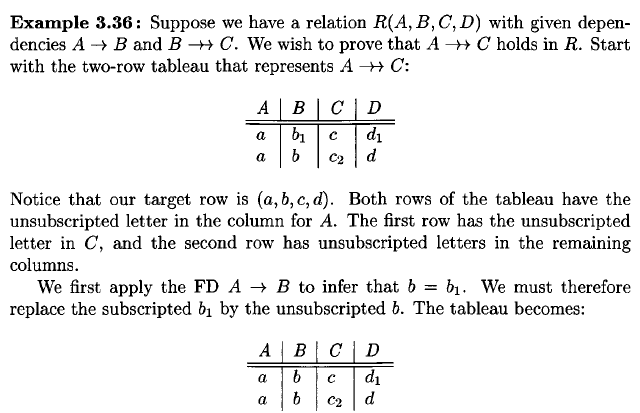
\includegraphics[scale=0.7]{chase_tableau_dmv_1}
\end{figure}

\begin{figure}[H]
	\centering
	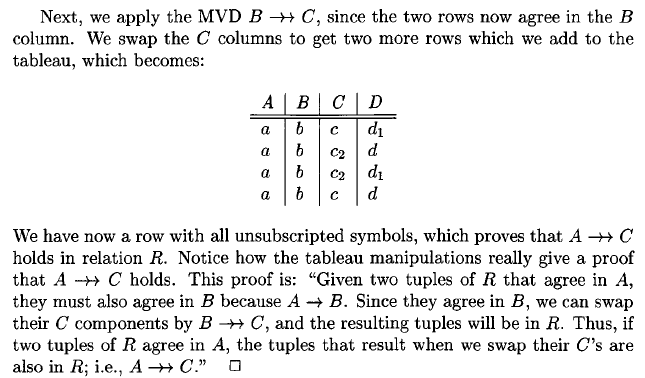
\includegraphics[scale=0.7]{chase_tableau_dmv_2}
\end{figure}

\newpage
\part{SQL}
Componentes: 
\begin{enumerate}
	\item DDL (\emph{Data Definition Language})
	\item DML (\emph{Data Manipulation Language})
	\item CL (\emph{Control Language})
\end{enumerate}

Para identificar unívocamente a una relación, se utiliza el formato \texttt{<catalogo>.<esquema>.<relación>}

\section{DDL}
\begin{description}
\item[DDL] Lenguaje de definición de datos para especificar el esquema de la base de datos, eliminar relaciones, modificar esquemas, crear vistas, crear restricciones de integridad, especificar derechos de acceso, etc.
\end{description}

\subsection{Tipos de dominios}
\begin{itemize}
\item \texttt{char($n$)}: texto de longitud $n$
\item \texttt{varchar($n$)}: texto de longitud variable, con un máximo
de $n$ caracteres
\item \texttt{nvarchar($n$)}: texto de longitud variable, con un máximo
de $n$ caracteres, utilizando el formato Unicode
\item \texttt{int}
\item \texttt{smallint}
\item \texttt{numeric($p$,$d$)}: $p$ dígitos con signo, y $d$ de los
$p$ dígitos están a la derecha del punto decimal.
\item \texttt{real, double precision}
\item \texttt{float($n$)}
\item \texttt{date}
\item \texttt{time}
\item \texttt{timestamp}
\item \texttt{clob(n)}: character large object de $n$ bytes
\item \texttt{blob(n)}: binary large object de $n$ bytes
\end{itemize}

\subsection{Create table}

\begin{lstlisting}
CREATE TABLE r(A1 D1, A2 D2, ..., An Dn,
		<restriccion-integridad1>,
		...,
		<restriccion-integridadK>);
\end{lstlisting}


La instrucción anterior crea una tabla llamada \emph{r} con atributos
$A_{i}$, y $D_{i}$ es el dominio del atributo $A_{i}$.

Las restricciones de integridad pueden ser:
\begin{itemize}
\item \texttt{primary key ($A_{j1},A_{j2},\dots,A_{jm})$}: los atributos
$A_{ji}$, con $i\in[1,m]$ forman la clave primaria de cada tupla.
No pueden ser \emph{null}, y deben ser únicos.
\item \texttt{check ($P$)}: todas las tuplas de $r$ deben satisfacer el
predicado $P$.
\item \texttt{foreign key}:\texttt{}
\begin{lstlisting}
FOREIGN KEY (atr) REFERENCES rel
	ON [update|delete] [cascade|set null|set default];
\end{lstlisting}



Se establece que el atributo \texttt{atr} es una clave primaria en
la relación \texttt{rel}. Se puede especificar lo que sucede si se
produce una actualización o un borrado de dicho valor en la relación
\texttt{rel}:
\begin{itemize}
\item \textbf{Cascade}: se actualiza/elimina la tupla en esta relación
\item \textbf{Set null}: la clave foránea se establece en \emph{null}
\item \textbf{Set default}: la clave foránea se establece en su valor por
default
\end{itemize}
\item \texttt{assert}: define una restricción aplicable a varias tablas.


\begin{lstlisting}
CREATE ASSERTION nombre_asercion
	CHECK P
\end{lstlisting}


\end{itemize}

\subsection{Drop table}

La instrucción \texttt{DROP TABLE r} elimina todas las tuplas de la
tabla $r$ y el esquema de relación $r$.


\subsection{Alter table}

La instrucción puede utilizarse para agregar atributos nuevos (con
valor \emph{null}) o para eliminarlos.

\begin{lstlisting}
ALTER TABLE r 
	ADD <Atributo> <Dominio>;
ALTER TABLE r 
	DROP <Atributo>;
\end{lstlisting}

\begin{description}
\item [{Diccionario~de~datos}] Contiene \textbf{metadatos} (información
sobre los datos), en particular, sobre el esquema de la misma.
\end{description}

\section{DML}
\begin{description}
\item [{DML}] Lenguaje de manipulación de datos para expresar las consultas
a la base de datos.
\end{description}
Operaciones CRUD (\emph{Create}, \emph{Read}, \emph{Update}, \emph{Delete})
\begin{description}
\item [{%
\begin{tabular}{|c|c|}
\hline 
\emph{Álgebra relacional} & \emph{SQL}\\
\hline 
\hline 
$\pi_{attr}(r)$ & \texttt{SELECT attr FROM r}\\
\hline 
$\sigma_{cond}(r)$ & \texttt{SELECT {*} FROM r WHERE cond}\\
\hline 
$r\times s$ & \texttt{SELECT {*} FROM r,s}\\
\hline 
\end{tabular}}]~
\end{description}
La expresión

\begin{lstlisting}
SELECT a1, a2, ..., an
FROM r1, r2, ..., rm
WHERE p;
\end{lstlisting}


es equivalente a la expresión $\pi_{a_{1},a_{2},\dots,a_{n}}\left(\sigma_{p}\left(r_{1}\times r_{2}\times\dots\times r_{m}\right)\right)$.
\begin{itemize}
\item El resultado de una expresión SQL \textbf{puede} contener tuplas duplicadas.
Para eliminar los duplicados, se utiliza la cláusula \texttt{SELECT
DISTINCT}.
\item Las funciones agregadas no se pueden componer. Por ejemplo, \texttt{max(count({*}))}
no es válido.
\item Una cláusula de tipo \texttt{SELECT {*}} indica que se seleccionan
todos los atributos de las relaciones en la cláusula \texttt{FROM}.
\item El operador de renombre \texttt{as}: \texttt{SELECT viejo-nombre AS
nuevo-nombre}
\item El operador \texttt{like} se puede usar dentro de una cláusula \texttt{where}
para buscar valores que cumplan un patrón, especificado con los siguientes
caracteres especiales: 

\begin{itemize}
\item \texttt{\%}: matchea cualquier sub string
\item \texttt{\_}: matchea un caracter cualquiera
\end{itemize}
\item El operador \texttt{order by <atributo(s)> {[}asc|desc{]}} ordena
el resultado de una consulta por uno o varios de los atributos, de
forma ascendente o descendente (ascendente por default).
\item Operadores sobre conjuntos:

\begin{itemize}
\item \texttt{Union}
\item \texttt{Intersect}
\item \texttt{Except}
\end{itemize}
\item El operador \texttt{group by} permite agrupar tuplas en base a uno
o más atributos (las tuplas con el mismo valor para los atributos
en esta cláusula se ponen en un mismo grupo). Los atributos en la
cláusula \texttt{select}, por fuera de las funciones agregadas, deben
estar en el operador \texttt{group by}. La sintaxis es:


\begin{lstlisting}
SELECT expr1, ..., exprN, funcionAgregada(expr)
FROM tablas
WHERE condiciones
GROUP BY expr1, ..., exprN;
\end{lstlisting}



\emph{Ejemplo: encontrar el promedio del saldo de las cuentas en cada
sucursal de un banco.}


\begin{lstlisting}
SELECT sucursal-nombre, avg(saldo)
FROM cuentas
GROUP BY sucursal-nombre;
\end{lstlisting}


\item El operador \texttt{having} permite seleccionar a grupos formados
con \texttt{group by }que cumplan una condición. Cualquier atributo
que esté presente en la cláusula \texttt{having} sin agregar, debe
aparecer en el operador \texttt{group by}.


\begin{lstlisting}
SELECT columna, funcion_agregada(columna) 
FROM tabla 
WHERE columna operator value 
GROUP BY columna
HAVING funcion_agregada(columna) operator value;
\end{lstlisting}



\emph{Ejemplo: encontrar los nombres de las sucursales del banco que
tengan un promedio general de saldo mayor a \$1200.}


\begin{lstlisting}
SELECT sucursal-nombre
FROM cuentas
GROUP BY sucursal-nombre
HAVING avg(saldo) > 1200
\end{lstlisting}


\end{itemize}
\textbf{Nota}: si se utilizan el operador \texttt{where} y el operador
\texttt{having}, primero se aplica el \texttt{where} y luego se filtra
por \texttt{having}.


\subsection{Consultas anidadas}

En una consulta anidada, el \texttt{select} interno puede tener variables
de tuplas definidas dentro del \texttt{select}, o en cualquier consulta
que incluya a ésta.
\begin{itemize}
\item El conector \texttt{in} permite verificar la pertenencia de un valor
a un conjunto que es resultado de una cláusula \texttt{select}. De
forma equivalente, existe el conector \texttt{not in}.


\emph{Ejemplo: encontrar los nombres de los clientes que tienen un
préstamo y una cuenta en el banco.}


\begin{lstlisting}
SELECT DISTINCT cliente-nombre
FROM pidio-prestamo
WHERE cliente-nombre IN (SELECT cliente-nombre
			FROM tiene-cuenta);
\end{lstlisting}


\item El operador de comparación \texttt{some} en una cláusula \texttt{where}
de un \texttt{select} externo devuelve verdadero si el valor del atributo
en cuestión es mayor o menor que al menos un valor de la cláusula
\texttt{select} interna.


\emph{Ejemplo: encontrar los nombres de las sucursales del banco que
tienen activos mayores que los de al menos una sucursal en Brooklyn.}


\begin{lstlisting}
SELECT sucursal-nombre
FROM sucursales
WHERE activos > SOME (SELECT activos
			FROM sucursales
			WHERE sucursal-nombre = 'Brooklyn');
\end{lstlisting}


\item El operador de comparación \texttt{all} en una cláusula \texttt{where}
de un \texttt{select} externo devuelve verdadero si el valor del atributo
en cuestión es mayor a todos los valores de la cláusula \texttt{select}
interna.


\emph{Ejemplo: encontrar los nombres de las sucursales del banco que
tienen activos mayores que los todas las sucursales en Brooklyn.}


\begin{lstlisting}
SELECT sucursal-nombre
FROM sucursales
WHERE activos > ALL (SELECT activos
			FROM sucursales
			WHERE sucursal-nombre = 'Brooklyn');
\end{lstlisting}


\item El operador \texttt{any} devuelve verdadero si existe al menos un
valor para


\emph{Ejemplo: encontrar los clientes que pidieron un préstamo de
monto mayor a al menos los activos de una sucursal.}


\begin{lstlisting}
SELECT cliente-nombre
FROM pidio-prestamo
WHERE cantidad > ANY (SELECT activos
			FROM sucursales);
\end{lstlisting}


\item El operador \texttt{exists} devuelve verdadero si la consulta interna
no es vacía.


\emph{Ejemplo: encontrar los clientes que tienen una cuenta y un préstamo
en el banco.}


\begin{lstlisting}
SELECT cliente-nombre
FROM pidio-prestamo
WHERE EXISTS (SELECT *
		FROM tiene-cuenta
            WHERE pidio-prestamo.cliente-nombre = tiene-cuenta.cliente-nombre);
\end{lstlisting}


\item El operador \texttt{unique} devuelve verdadero si la consulta interna
no contiene tuplas duplicadas.
\end{itemize}
SQL no ofrece en forma nativa la posibilidad de ejecutar el operador
división. Sin embargo, este se puede implementar usando consultas
anidadas.

\emph{Ejemplo: dados los siguientes esquemas relacionales}

\begin{lstlisting}
Estudiante (Enro, Enombre, Carrera, Anio_cursa, Edad) 
Curso (Cnombre, Horario, Aula, Pid) 
Cursa (Enro, Cnombre) 
Profesor (Pid, Pnombre, departamento) 
\end{lstlisting}


\emph{Hallar los nombres de todos los profesores que enseñan en todas
las aulas en las que se dicta algún curso.}

\begin{lstlisting}
SELECT P.Pnombre 
FROM Profesor P 
WHERE NOT EXISTS (SELECT C.Aula                   
				FROM Curso C1                  
				WHERE NOT EXISTS (SELECT *                                    
								FROM Curso C2                                    
								WHERE C2.Aula = c1.Aula AND      
                                    C2.Pid = P.Pid));
\end{lstlisting}



\subsection{Delete}

Sintaxis para el borrado de tuplas de la relación $r$ para las cuales
$P$ es verdadera:

\begin{lstlisting}
DELETE FROM r
WHERE P
\end{lstlisting}

\begin{itemize}
\item Sólo se borra de una relación.
\item Sólo se borran tuplas (no atributos de tuplas).
\item Primero se buscan todas las tuplas que satisfacen $P$, y luego se
borran todas ellas.
\end{itemize}

\subsection{Insert}

Sintaxis para la inserción de tuplas en la relación $r$:

\begin{lstlisting}
INSERT INTO r (nombreAtributo1, ..., nombreAtributoN)
VALUES (valor1, ..., valorN)
\end{lstlisting}


\begin{lstlisting}
INSERT INTO r 
	SELECT (...)
\end{lstlisting}

\begin{itemize}
\item Primero se buscan todas las tuplas que satisfacen el \texttt{select},
y luego se insertan todas ellas.
\end{itemize}

\subsection{Update}

Sintaxis para la actualización de un atributo de una tupla de $r$:

\begin{lstlisting}
UPDATE r
SET atributo = valor
WHERE condicion
\end{lstlisting}


\begin{lstlisting}
UPDATE r
SET atributo = CASE
				WHEN condicion1 THEN valor1
				WHEN condicion2 THEN valor2
				ELSE valor3
			   END
\end{lstlisting}


\pagebreak{}


\part{Procesamiento de Consultas}

\noindent \begin{center}
\begin{figure}[H]
\noindent \begin{centering}
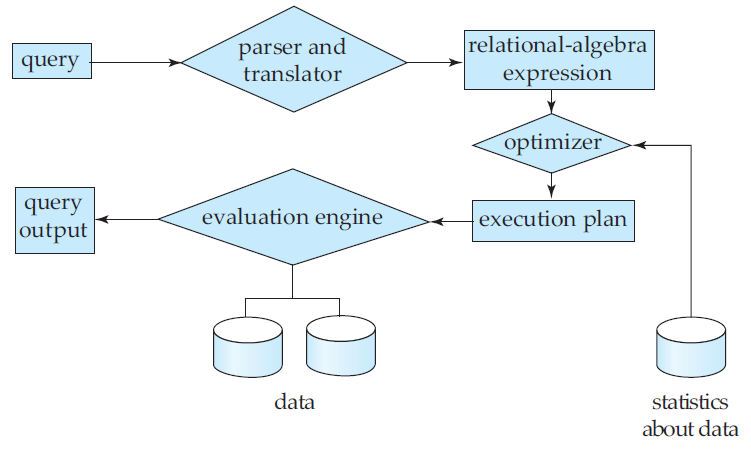
\includegraphics[scale=0.5]{proc_consultas}
\par\end{centering}

\protect\caption{Pasos en el procesamiento de consultas}
\end{figure}

\par\end{center}

Asumimos que toda la relación se almacena de forma contigua en disco.

Metadatos que se almacenan para cada base de datos:
\begin{enumerate}
\item $n_{r}=$ cantidad de tuplas en la relación $r$
\item $l_{r}=$ tamaño de una tupla, en bytes
\item $b_{r}=$ cantidad de bloques que ocupa la relación $r$. 
\[
b_{r}=\frac{l_{r}\times n_{r}}{tam\, bloque\, en\, bytes}
\]

\item $f_{r}=$ factor de bloqueo de la relación $r$ (es decir, cuantas
tuplas caben en un bloque)


\[
f_{r}=\left\lceil \frac{n_{r}}{b_{r}}\right\rceil 
\]


\item $V(A,r)=$cantidad de valores distintos que toma el atributo $A$
en la relación $r$
\item $MIN(A,r)=$mínimo valor que toma el atributo $A$ en la relación
$r$
\item $MAX(A,r)=$máximo valor que toma el atributo $A$ en la relación
$r$
\end{enumerate}
\begin{figure}[H]
\noindent \begin{centering}
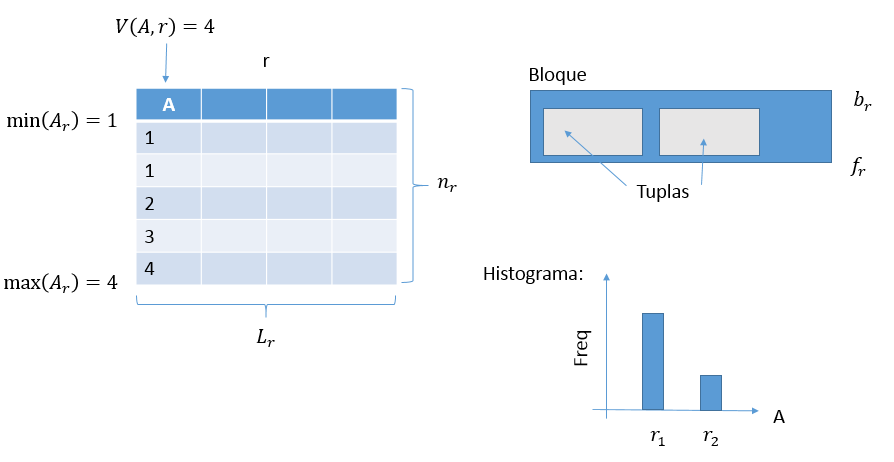
\includegraphics[scale=0.5]{info_db}
\par\end{centering}

\protect\caption{Estadísticas que se almacenan de la base de datos}
\end{figure}



\section{Índices}

Ciertas consultas sobre algunos atributos son más frecuentes que otras.
Para acelerar estas consultas, se utilizan los índices. Podemos tener
más de un índice sobre una relación.
\begin{description}
\item [{Índice}] Estructura de datos (usualmente árbol B+) que permiten
encontrar rápidamente las tuplas de una relación que tengan un valor
especifico para un atributo o atributos (el/los que el índice almacena),
con la desventaja de que cada modificación a la relación requiere
actualizar el índice.


Un registro de un índice tiene un valor de la clave de búsqueda, y
punteros a uno o más tuplas con esa clave de búsqueda.

\end{description}
\begin{lstlisting}
CREATE [CLUSTERED] INDEX estudianteID_indice
	ON estudiante
{
	ID asc
};
\end{lstlisting}


Tipos de índices:
\begin{itemize}
\item Según la clave:

\begin{itemize}
\item \textbf{Clusterizado} \textbf{/ primario}: índice cuya clave de búsqueda
define el orden secuencial del archivo de la tabla. Sólo puede haber
uno de estos índices para cada relación
\item \textbf{Clusterizado / secundario}.

\begin{itemize}
\item El orden físico de las tuplas no es igual al orden del índice
\item Las columnas que se indexan son, típicamente, atributos no claves
\item Siempre son densos
\end{itemize}
\end{itemize}
\item Según la cantidad de registros que tiene:

\begin{itemize}
\item \textbf{Denso}: tiene un registro para cada valor posible de la clave
de búsqueda. Si es clusterizado, tiene un puntero al primer registro
con ese valor. Si es no clusterizado, tiene punteros a todos los registros
con ese valor.
\item \textbf{Esparcido}: tiene registros para algunos valores de la clave
de búsqueda. Solo se pueden usar si el archivo de datos está ordenado
por la clave de búsqueda.
\end{itemize}
\end{itemize}
\noindent \begin{center}
$Esparcido\implies Primario$
\par\end{center}

\noindent \begin{center}
$Secundario\implies Denso$
\par\end{center}

\begin{figure}[H]
\subfloat[Índice denso]{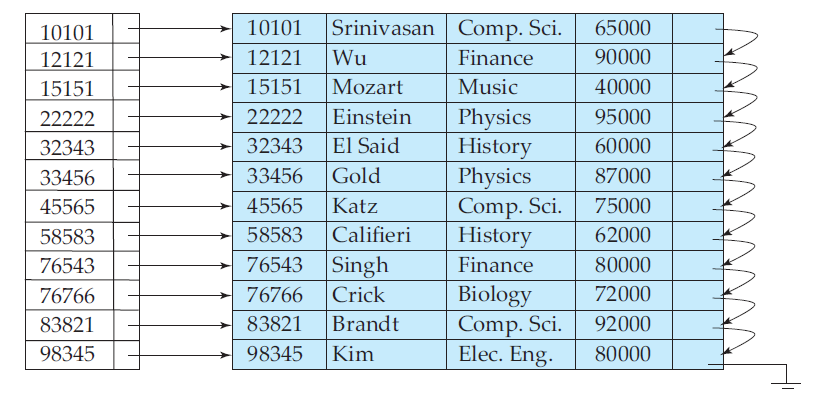
\includegraphics[scale=0.4]{dense_index}



}\subfloat[Índice esparcido]{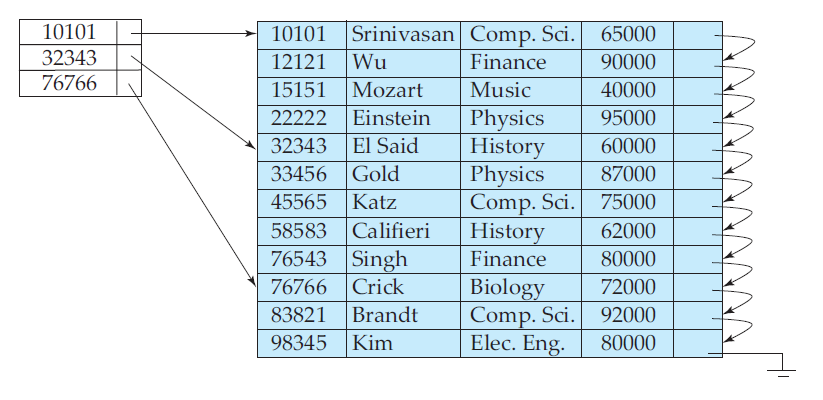
\includegraphics[scale=0.4]{sparse_index}

}

\protect\caption{Índices densos y esparcidos}


\end{figure}

\begin{description}
\item [{Índice~compuesto}] índice cuya clave de búsqueda está formada
por más de un atributo. Conviene que los atributos de más a la izquierda
sean más discriminantes que los de la derecha. \emph{Ejemplo: para
una relación $pelicula(nombre,a\tilde{n}o)$, es esperable que haya
más consultas sobre el $nombre$ que sobre el $a\tilde{n}o$. Entonces,
un índice $(nombre,a\tilde{n}o)$ sería mejor que $(a\tilde{n}o,nombre).$}
\item [{Índice~cubridor}] Es un índice que contiene todas las columnas
de una consulta, y por ende no se necesita realizar búsquedas adicionales
en el índice clusterizado.
\end{description}

\subsection{Estructuras de índices}
\begin{itemize}
\item Árbol B+
\item Tabla de hash
\end{itemize}
\noindent \begin{center}
\begin{tabular}{|c|c|c|}
\hline 
 & \textbf{Ventajas} & \textbf{Desventajas}\\
\hline 
\hline 
\textbf{Árbol B+} & Soporta búsquedas por rango & Operaciones más costosas\\
\hline 
\textbf{Tabla de hash} & La búsqueda típica requiere solo una operación de I/O & No soporta búsquedas por rango. \\
\hline 
\end{tabular}
\par\end{center}


\section{Formas de realizar consultas}
\begin{enumerate}
\item Búsqueda lineal sobre toda la relación
\item Usando índices
\item \emph{Hashing}
\item Ordenamiento
\end{enumerate}
Los algoritmos pueden asumir que una relación entra completamente
en memoria, o que son muy grandes.


\subsection{Operadores}
\begin{itemize}
\item \emph{Scan}

\begin{itemize}
\item \emph{Table scan}: se leen todos los bloques de la relación en disco.
\item \emph{Index scan}: se leen todos los bloques de la relación en disco,
utilizando un índice.
\item \emph{Sort scan:} ordena una relación $R$ sobre un atributo $a$.

\begin{itemize}
\item Si hay un índice sobre $a$, se lo usa.
\item Si $R$ entra en memoria, se la trae a memoria con \emph{table} o
\emph{index scan}, y se la ordena en memoria
\item Si $R$ no entra en memoria, se la ordena externamente.
\end{itemize}
\end{itemize}
\end{itemize}

\section{Algoritmos}


\subsection{Selección}

$\sigma_{A=a}(r)$
\begin{itemize}
\item Búsqueda lineal sobre $r$:

\begin{itemize}
\item Si la relación es clusterizada: $b_{r}$
\item Si la relación no está clusterizada: $n_{r}$
\end{itemize}
\item Búsqueda con índice sobre los atributos de $A$:

\begin{itemize}
\item Si el índice es clusterizado: costo $\frac{b_{r}}{V(A,r)}$
\item Si el índice no es clusterizado: costo $\frac{n_{r}}{V(A,r)}$
\end{itemize}
\end{itemize}

\subsection{Junta}

$R(X,Y)\bowtie S(Y,Z)$, donde $R$ es la relación más pequeña. Suponemos
que la memoria está formada por $M$ buffers.
\begin{itemize}
\item Iteración ingenua (\emph{tuple based nested-loop join}): 

\begin{itemize}
\item costo $n_{s}\times n_{r}$
\end{itemize}

\begin{lstlisting}
para cada tupla s en S:
	para cada tupla r en R:
		si (s join r = t):
			devolver t
\end{lstlisting}


\item Iteración por bloques (\emph{block based nested-loop join}): 

\begin{itemize}
\item Costo $b_{r}+\frac{b_{r}}{m-1}\times b_{s}$ ($R$ se lee una vez,
$S$ se lee por cada pedazo de $R$, cada pedazo es de tamaño $\frac{b_{r}}{m-1}$)
\item Conviene que la relación del ciclo externo sea la más pequeña
\end{itemize}

\begin{lstlisting}
desde i=1 hasta i=(bR / m-1):
	leer R en memoria (ocupar M-1 buffers)
	para cada bloque bs en S:
		leer bs en memoria (ocupar 1 buffer)
		para cada tupla t en bs:
			buscar las tuplas de R en que hacen join con t
			devolver t
\end{lstlisting}


\item \emph{Indexed nested-loop join}: suponer que se tiene un índice sobre
$S$ del atributo $Y$.

\begin{itemize}
\item Si el índice es clusterizado: costo $b_{r}+\frac{n_{r}b_{s}}{V(Y,S)}$
\item Si el índice no es clusterizado: costo $b_{r}+\frac{n_{r}n_{s}}{V(Y,S)}$
\item Este método es eficiente cuando $S$ no está almacenada en forma contigua
en disco.
\end{itemize}

\begin{lstlisting}
para cada bloque br de R:
	para cada tupla t de br:
		buscar con el indice las tuplas de S que hacen join con t
		para cada tupla s join t:
			agregar <s,t> al resultado
\end{lstlisting}


\item Sort-merge (\emph{sort based join}): 

\begin{itemize}
\item Costo $b_{s}+b_{r}+b_{s}\log(b_{s})+b_{r}\log(b_{r})$
\end{itemize}

\begin{lstlisting}
ordenar R con respecto a Y
ordenar S con respecto a Y
mergear R y S:
	encontrar min(R) y min(S)
	si min(R) > min(S)
		quitar las tuplas de S con Y como atributo
		leer S
	si min(R) < min(S)
		quitar las tuplas de R con Y como atributo
		leer R
	si min(R) == min(S)
		agregar r join s al resultado
		leer R
		leer S
\end{lstlisting}


\item Método Simple de Junta Hash: utiliza una función de hash $h$. Requiere
que la relación $R$ entre en memoria. $h\to[0,M-1]$.

\begin{itemize}
\item Costo: $2\left(b_{r}+b_{s}\right)$
\end{itemize}

\begin{lstlisting}
TH = {} // en memoria

// fase constructiva
para cada bloque de R:
	para cada tupla r del bloque:
		calcular h(r[Y])
		guardar TH[Y] = r

// fase exploratoria
para cada bloque de S:
	para cada tupla s del bloque:
		calcular h(s[Y])
		agregar al resultado las tuplas de TH[Y] join "s"
\end{lstlisting}


\item Método GRACE:


El método de junta Hash versión GRACE se usa para calcular la junta
$R\bowtie_{R.A=S.A}S$ cuando ninguna de las tablas entran en memoria.
Lo que se hace es generar 2 conjuntos de $M$ particiones. Se utilizan
dos funciones de hash: una para generar las particiones $h:A\to[0,M-1]$,
y otra para calcular qué tuplas hacen \emph{join}.


En una primera etapa, por cada tupla $t$ de cada bloque de $R$ se
aplica la función de hashing $h(t)$ para saber a cuál partición enviar
la tupla. Se envía cada tupla a esa partición (un archivo) en disco.
Al finalizar la etapa, se tienen $M$ archivos.


En una segunda etapa, se hace lo mismo con $S$, pero con otros $M$
archivos. La clave está en que si dos tuplas hacen \emph{join}, entonces
necesariamente deben estar en el mismo número de partición. 


Finalmente, se leen las $i$ particiones. A cada tupla leída de la
partición $i$ de $R$ se le aplica la función de hash $h_{2}$ para
saber dónde guardarla en una tabla de hash en memoria. Luego, se calcula
$h_{2}$ para cada tupla de la partición $i$ de $S$. Este valor
nos dirá la posición en la tabla de hash donde están las tuplas de
$R$ que hacen \emph{join} con dicha tupla. De esta forma se obtienen
las tuplas que hacen \emph{join}, y se las graba en disco.
\begin{itemize}
\item Costo: $3\left(b_{s}+b_{r}\right)$
\end{itemize}

\begin{lstlisting}
// particionamiento de R. Costo: 2*bR
para cada tupla r de R:
	num buffer = calcular h1(r[Y])
	guardar "r" en el buffer
	si (buffer completo)
		guardarlo en disco Ri
// particionamiento de S. Costo: 2*bS
para cada tupla s de S:
	num buffer = calcular h1(s[Y])
	guardar "s" en el buffer
	si (buffer completo)
		guardarlo en disco Si

// metodo simple de hash. Costo: bR + bS
para i desde 0 a M-1:
	leer Ri
	para cada tupla r en Ri:
		calcular h2(r[Y])
		guardar TH[r[Y]] = r
	leer Si
	para cada tupla s en Si:
		calcular h2(s[Y])
		agregar al resultado las tuplas de TH[r[Y]] join "s"
\end{lstlisting}


\end{itemize}

\section{Evaluación de expresiones}

La forma obvia de evaluar una expresión que tiene varias operaciones
es evaluar cada operación en el orden indicado, materializando en
disco cada resultado intermedio como relaciones temporales.

Otra alternativa, más eficiente, es evaluar las operaciones en simultáneo
en un \textbf{pipeline}, donde los resultados de una operación pasan
a la próxima, y se elimina la necesidad de almacenar relaciones temporales.
Esto se puede utilizar para evaluar juntas múltiples: $R_{1}\bowtie R_{2}\bowtie\cdots\bowtie R_{k}$.

Ventajas de \emph{pipeline:}
\begin{enumerate}
\item Elimina el costo de leer y escribir relaciones temporales.
\item Puede empezar a generar resultados inmediatamente.
\end{enumerate}
Uso de \emph{pipelining}:
\begin{itemize}
\item \emph{Sort}: no se puede aplicar. El resultado del sort no se puede
mostrar hasta que no se hayan procesado todas las tuplas.
\item \emph{Join}: el método GRACE no se puede aplicar porque requiere leer
y particionar todas las tuplas antes de que pueda producirse un resultado.
Sin embargo, el método \emph{indexed nested-loop} puede aprovechar
del \emph{pipelining. }Si las relaciones están ordenadas por los atributos
de join, merge join también puede aprovechar del \emph{pipelining.}
\end{itemize}

\section{Optimización de consultas}
\begin{description}
\item [{Plan~de~evaluación}] conjunto de operaciones de álgebra relacional
a ejecutar, junto con las instrucciones para llevarlas a cabo (por
ejemplo, los índices a usar).
\item [{Optimización~de~consultas}] proceso de seleccionar el mejor plan
de evaluación. El costo de cada plan se evalúa teniendo en cuenta
información estadística de las relaciones. Lo que se busca minimizar
es la cantidad de transferencias de bloques del disco a la memoria
y la cantidad de \emph{seeks} que se hacen en el disco. 


Para ello se tiene en cuenta:
\begin{enumerate}
\item ¿Cuál de la de las expresiones equivalentes a la consulta es más eficiente
para resolver la misma?
\item ¿Qué algoritmo se utilizará para implementar la operación?
\item ¿Cómo deberían las operaciones pasarse datos entre sí? (\emph{Pipeline},
buffers de memoria, disco)
\end{enumerate}
\end{description}
\begin{lstlisting}
EXPLAIN consulta
\end{lstlisting}
 


\subsection{Reglas de equivalencia}

Reglas relacionadas con la selección:
\begin{enumerate}
\item $\sigma_{a\wedge b}(r)=\sigma_{a}\left(\sigma_{b}(r)\right)=\sigma_{b}\left(\sigma_{a}(r)\right)$
\item $\sigma_{a\vee b}(r)=\sigma_{a}(r)\cup\sigma_{b}(r)$
\item $\sigma_{a}(r\cup s)=\sigma_{a}(r)\cup\sigma_{a}(s)$
\item $\sigma_{a}(r-s)=\sigma_{a}(r)-s=\sigma_{a}(r)-\sigma_{a}(s)$
\item $\sigma_{a}(r\bowtie s)=\sigma_{a}(r)\bowtie\sigma_{a}(s)$
\item Si $a$ solo tiene atributos de $S$: $\sigma_{a}(r\times s)=r\times\sigma_{a}(s)$
\end{enumerate}
Reglas relacionadas con la proyección:
\begin{enumerate}
\item $\pi_{L}(R\cup S)=\pi_{L}(R)\cup\pi_{L}(S)$
\item $\pi_{L}\left(\sigma_{a}(R)\right)=\pi_{L}\left(\sigma_{a}\left(\left(\pi_{M}(R)\right)\right)\right)$
donde $M$ es la lista de atributos que figuran en $L$ o en $a$
\end{enumerate}
Reglas relacionadas con el \emph{join}:
\begin{enumerate}
\item $r_{1}\bowtie r_{2}=r_{2}\bowtie r_{1}$
\item $\left(r_{1}\bowtie r_{2}\right)\bowtie r_{3}=r_{1}\bowtie\left(r_{2}\bowtie r_{3}\right)$
\end{enumerate}

\subsection{Heurísticas de optimización de consultas}
\begin{enumerate}
\item Ejecutar las selecciones $(\sigma)$ lo antes posible 
\item Ejecutar las proyecciones $(\pi)$ lo antes posible
\item El orden de las operaciones de \emph{join} $(\bowtie)$ es importante
\item Evitar cuando sea posible los productos cartesianos $(\times)$
\end{enumerate}

\section{Estimación de tamaño de consultas}

A continuación se describe la estimación de cantidad de tuplas para
cada tipo de consulta. 

Se utiliza el concepto de \textbf{selectividad} de una condición $A$
como la ``probabilidad de que una tupla satisfaga una condición $A$''.
Sea $s_{i}=V(\sigma_{i},r)$ la cantidad de tuplas que satisfacen
la condición $\sigma_{i}$. La probabilidad de satisfacer $\sigma_{i}$
es $\frac{s_{i}}{n_{r}}$.
\begin{itemize}
\item Selección

\begin{itemize}
\item $\sigma_{A=a}(r)$

\begin{itemize}
\item Si $A$ distribuye uniformemente: $\frac{n_{r}}{V(A,r)}$
\item Si se dispone de un histograma para $A$, y $a\in rango$: $\frac{freq_{rango}(A,r)}{cant_{rangos}}$
\end{itemize}
\item $\sigma_{A\leq v}(r)$ con $v$ conocido

\begin{itemize}
\item Si $A$ distribuye uniformemente y $v<\min(A,r)$: $0$
\item Si $A$ distribuye uniformemente y $v\geq\max(A,r)$: $n_{r}$
\item En cualquier otro caso: $n_{r}\cdot\frac{v-min(A,r)}{max(A,r)-min(A,r)}$
\end{itemize}
\item $\sigma_{a\wedge b\wedge\cdots\wedge z}(r)$ donde hay $x$ selectores:
$n_{r}\times P(a)\times\cdots\times P(z)=n_{r}\cdot\frac{s_{a}\cdot s_{b}\cdots s_{z}}{\left(n_{r}\right)^{x}}$
\item $\sigma_{a\lor b\lor\cdots\lor z}(r)$ donde hay $x$ selectores independientes
entre sí: 
\[
n_{r}\times\left[P(a)+\cdots+P(z)\right]=n_{r}\cdot\left[1-\left(1-\frac{s_{a}}{n_{r}}\right)\times\cdots\times\left(1-\frac{s_{z}}{n_{r}}\right)\right]
\]

\item $\sigma_{\lnot a}(r)$: $n_{r}-V(a,r)$
\end{itemize}
\item Junta natural%
\footnote{Se introducen dos simplificaciones:
\begin{enumerate}
\item Si $R(X,Y)$ y $S(Y,Z)$, y $V(R,Y)\leq V(S,Y)$ entonces cada valor
de $Y$ en $R$ será un valor de $Y$ en $S$.
\item Si $A$ es un atributo de $R$ pero no de $S$, $V\left(R\bowtie S,A\right)=v\left(R,A\right)$\end{enumerate}
%
}

\begin{itemize}
\item Si $R\cap S=\emptyset$: $n_{r}\times n_{s}$
\item Si $R\cap S=PK_{R}:$ $\leq n_{S}$ (porque podría haber \emph{nulls})
\item Si $R\cap S=PK_{S}:$ $\leq n_{R}$ (porque podría haber \emph{nulls})
\item Si $R\cap S=FK_{S}:$ $n_{S}$
\item Si $R\cap S=FK_{R}:$ $n_{R}$
\item Si $\#(R\cap S)=1$: $\frac{n_{s}\times n_{r}}{\max\left(V(S,R\cap S),V(R,R\cap S)\right)}\approx\frac{n_{s}\times n_{r}}{V(S,R\cap S)}\approx\frac{n_{s}\times n_{r}}{V(R,R\cap S)}$
\item Si $\#(R\cap S)=2$ y el \emph{join} es de tipo $R.A_{1}=S.A_{2}\wedge R.B_{1}=S.B_{2}$:
\[
\frac{n_{r}\times n_{s}}{\max\left(V(R,A_{1}),V(S,A_{2}\right)\times\max\left(V(R,B_{1}),V(S,B_{2})\right)}
\]

\end{itemize}
\item Proyección: $\pi_{A}(r):$ $V(A,r)$
\item Agregación $_{A}\varrho_{f}(r):$ $V(A,r)$
\item Unión $R\cup S$: $n_{r}+n_{s}$
\item Intersección $R\cap S:$ $\min\left(n_{r},n_{s}\right)$ (cota superior)
\item Diferencia $R-S:$ $r$ (cota superior)
\item $V\left(A,\sigma_{A\, op\, v}(r)\right):$ $V(A,r)\times s_{A\, op\, v}$
\item $V\left(A,r\bowtie s\right):$ 

\begin{itemize}
\item Si $A\in R$: $\min\left(V(A,r),n_{r\bowtie s}\right)$
\item Si $a_{1}\in A$ y $a_{2}\in A$, $\min\left(V(a_{1},r)\times V(a_{2}-a_{1},s);V(a_{1}-a_{2},r)\times V(a_{2},S);n_{r\bowtie s}\right)$
\end{itemize}
\end{itemize}

\subsection{Cálculo de juntas con histogramas}

Un sistema de bases de datos puede computar un histograma de valores
para un atributo dado. Si $V(R,A)$ no es muy grande, el histograma
puede consistir de la cantidad de tuplas que tienen cada posible valor
del atributo. Si $V(R,A)$ es muy grande, entonces podría guardarse
solamente los valores más frecuentes, o agruparlos en rangos.

Los tipos de histogramas más frecuentes son:
\begin{enumerate}
\item \textbf{Igual ancho:} se escoge un ancho $w$ y una constante $v_{0}$.
Se almacena la cantidad de tuplas con valores $v$ en los rangos\emph{
$v_{0}\leq v<v_{0}+w,$ $v_{0}+w\leq v<v_{0}+2w$}, etcétera\emph{.}
\item \textbf{Valores más frecuentes}: se listan los valores más frecuentes
y la cantidad de tuplas que tienen esos valores. También se puede
proporcionar la cantidad de tuplas que tienen ``otros'' valores.
\end{enumerate}
\emph{\uline{Ejemplo}}\emph{: sea la junta $R(A,B)\bowtie S(B,C)$.
Sabemos que $V(R,B)=14$ y que $V(S,B)=13$. Tenemos los histogramas
de valores más frecuentes para $R\cap S=B$.}

\noindent \begin{center}
\emph{}%
\begin{tabular}{|c|c|c|c|c|c|}
\hline 
 & \emph{0} & \emph{1} & \emph{2} & \emph{5} & \emph{``Otros''}\\
\hline 
\hline 
\emph{$R.B$} & \emph{150} & \emph{200} & \emph{?} & \emph{100} & \emph{550 (11 valores)}\\
\hline 
\emph{$S.B$} & \emph{100} & \emph{80} & \emph{70} & \emph{?} & \emph{250 (10 valores)}\\
\hline 
\end{tabular}
\par\end{center}

\emph{Suponemos que cada valor que aparece en la relación con menos
valores de $B$ (en este caso, $S$) también aparecen en la otra relación
(en este caso, $R$). También suponemos que la distribución de los
valores dentro de ``Otros'' es uniforme, y estimamos la frecuencia
de los datos desconocidos:}

\noindent \begin{center}
\emph{}%
\begin{tabular}{|c|c|c|c|c|c|}
\hline 
 & \emph{0} & \emph{1} & \emph{2} & \emph{5} & \emph{Otros}\\
\hline 
\hline 
\emph{$R.B$} & \emph{150} & \emph{200} & \emph{$\frac{550}{11}=50$} & \emph{100} & \emph{550 (10 valores)}\\
\hline 
\emph{$S.B$} & \emph{100} & \emph{80} & \emph{70} & \emph{$\frac{250}{10}=25$} & \emph{250 (9 valores)}\\
\hline 
\end{tabular}
\par\end{center}

\emph{Entonces, el tamaño de la junta es:}

\emph{
\begin{eqnarray*}
T\left[R\bowtie S\right] & = & T\left[R\bowtie_{B=0}S\right]+T\left[R\bowtie_{B=1}S\right]+T\left[R\bowtie_{B=2}S\right]T\left[R\bowtie_{B=5}S\right]+T\left[R\bowtie_{B\neq0,1,2,5}S\right]\\
 & = & \left(150\times100\right)+\left(200\times80\right)+\left(50\times70\right)+\left(100\times25\right)+\min(9,10)\times\left(\frac{550}{11}\times\frac{250}{10}\right)\\
 & = & 15.000+16.000+3.500+2.500+9\times1250\\
 & = & 48.250
\end{eqnarray*}
}

\emph{\uline{Ejemplo}}\emph{: sean las relaciones $Enero(dia,temp)$
y $Julio(dia,temp)$. Sea la consulta}

\begin{lstlisting}
SELECT Enero.dia, Julio.dia
FROM Enero, Julio
WHERE Enero.temp = Julio.temp
\end{lstlisting}


\emph{Suponer los siguientes histogramas de igual ancho:}

\noindent \begin{center}
\emph{}%
\begin{tabular}{|c|c|c|}
\hline 
\emph{Rango C\textdegree{}} & \emph{Enero} & \emph{Julio}\\
\hline 
\hline 
\emph{-17, -13} & \emph{0} & \emph{40}\\
\hline 
\emph{-13, -9} & \emph{0} & \emph{60}\\
\hline 
\emph{-8, -4} & \emph{0} & \emph{80}\\
\hline 
\emph{-3, 1} & \emph{0} & \emph{50}\\
\hline 
\emph{2, 6} & \emph{5} & \emph{10}\\
\hline 
\emph{7, 11} & \emph{20} & \emph{5}\\
\hline 
\emph{12, 16} & \emph{50} & \emph{0}\\
\hline 
\emph{17, 21} & \emph{100} & \emph{0}\\
\hline 
\emph{22, 26} & \emph{60} & \emph{0}\\
\hline 
\emph{27, 31} & \emph{10} & \emph{0}\\
\hline 
\end{tabular}
\par\end{center}

\emph{Sabemos que si dos bandas tienen $T_{1}$ y $T_{2}$ tuplas
respectivamente, y la cantidad de valores de la banda es $V$, entonces
la estimación del tamaño de la junta es $\frac{T_{1}T_{2}}{V}$.}

\emph{En el ejemplo anterior, las únicas bandas que contribuyen al
resultado son las de {[}2,6{]} y {[}7,11{]}. Entonces, el tamaño de
la junta es:}

\emph{
\begin{eqnarray*}
T\left[R\bowtie S\right] & = & T\left[R\bowtie_{temp\in[2,6]}S\right]+T\left[R\bowtie_{temp\in[7,11]}S\right]\\
 & = & \frac{5\times10}{4}+\frac{20\times5}{4}\\
 & = & 12,5+25\\
 & = & 37,5
\end{eqnarray*}
}

\pagebreak{}


\part{Control de Concurrencia}
\begin{description}
\item [{Ítem~de~dato}] elemento al que accede una transacción. Puede
ser un registro de una base de datos, un bloque de disco, un campo
de un registro, o incluso toda la base de datos. Cada ítem tiene un
nombre único que lo identifica (por ejemplo, la dirección física de
un bloque de disco). 
\item [{Modelo~de~concurrencia~intercalada}] la CPU ejecuta una transacción
a la vez, pero varias transacciones en un período de tiempo.
\end{description}
\begin{figure}[H]
\noindent \begin{centering}
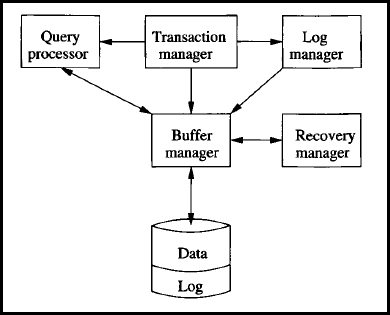
\includegraphics[scale=0.7]{transaction_manager}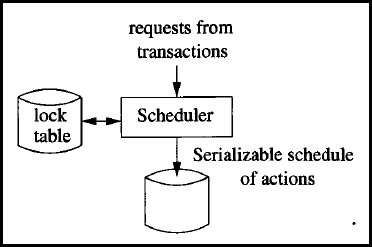
\includegraphics[scale=0.8]{scheduler}
\par\end{centering}

\protect\caption{El manejador de transacciones (a) le emite órdenes al manejador del
log, (b) se asegura que transacciones concurrentes no interfieran
entre ellas. El scheduler permite o bloquea transacciones}
\end{figure}



\section{Transacciones}
\begin{description}
\item [{Transacción}] unidad lógica de procesamiento. Está formada por
una o más operaciones que acceden a la base de datos. Tiene un identificador
único de transacción. 


Debe tener las siguientes propiedades \textbf{ACID}:
\begin{description}
\item [{%
\begin{tabular}{|c|>{\centering}m{7cm}|>{\centering}m{5cm}|}
\hline 
\emph{Atomicity} & La transacción debe ejecutarse en su totalidad o no debe ejecutarse & Responsabilidad del gestor de recuperación, que mantiene un log donde
guarda los valores viejos sobrescritos por una transacción \tabularnewline
\hline 
\emph{Consistency} & La transacción debe llevar a la base de datos de un estado consistente
a otro (i.e. que respeten las reglas de integridad de la base de datos) & Responsabilidad de los programadores \tabularnewline
\hline 
\emph{Isolation} & La ejecución de una transacción no debe interferir con otras & Responsabilidad del gestor de concurrencia \tabularnewline
\hline 
\emph{Durability} & Los efectos de una transacción commiteada deben persistir en la base
de datos. Es decir, luego de commiteada, no deberíamos necesitar ejecutar
un \emph{rollback} & Gestor de recuperación, que debe garantizar que el log esté en disco
antes de que termine la transacción \tabularnewline
\hline 
\end{tabular}}]~
\end{description}

\emph{How transactions interact with the database. There are three
address spaces that interact in important ways: }
\begin{enumerate}
\item \emph{The space of disk blocks holding the database elements.}
\item \emph{The virtual or main memory address space that is managed by
the buffer manager.}
\item \emph{The local address space of the transaction.}
\end{enumerate}

Cada transacción está formada por una o más operaciones:
\begin{itemize}
\item \texttt{\textbf{start}}
\item \texttt{\textbf{leer(X)}}: lee un item de dato de la base de datos
a una variable local a la transacción, que está en memoria
\item \texttt{\textbf{escribir(X)}}: escribe una variable de programa en
memoria, en la base de datos
\item \texttt{\textbf{commit}}: marca el fin exitoso de una transacción.
Los cambios que introdujo son seguros para guardar en la base de datos.
\item \texttt{\textbf{abort}}: marca el fin con errores de una transacción.
Los cambios que introdujo se deben revertir.
\end{itemize}

Estados posibles de una transacción:
\begin{itemize}
\item \textbf{\emph{Partially committed}}: luego de que se ejecutó la última
instrucción pero antes de ejecutar el \emph{commit} o \emph{abort}
\item \textbf{\emph{Commited}}: sus efectos fueron almacenados permanentemente
en la base de datos
\item \textbf{\emph{Aborted}}: se ejecutó un \emph{roll back} de la transacción
y la base de datos se restauró a su estado original


\begin{figure}[H]
\noindent \begin{centering}
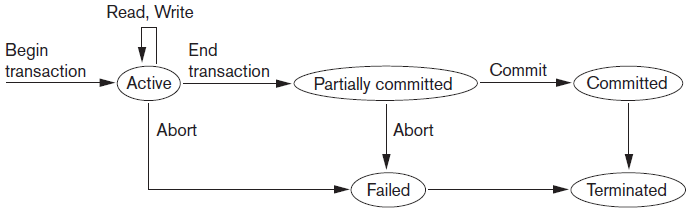
\includegraphics[scale=0.8]{state_diagram_transaction}
\par\end{centering}

\protect\caption{Diagrama de estados de una transacción}


\end{figure}


\end{itemize}

Una transacción llega al \textbf{punto de commit} cuando todas sus
operaciones se ejecutaron correctamente y se grabaron todos sus registros
de operaciones en el log. Luego de este punto, la transacción está
\textbf{commiteada} y se debe almacenar permanentemente en la base
de datos. Esto se marca agregando un registro \texttt{{[}commit,T{]}}
en el log.
\begin{enumerate}
\item Si ocurre una falla y la transacción aún no grabó \texttt{{[}commit,T{]}},
se debe ejecutar un \emph{rollback} de esta transacción.
\item Si ocurre una falla y la transacción ya había grabado \texttt{{[}commit,T{]}}
en el log, se debe \emph{rehacer} esta transacción.
\end{enumerate}

El protocolo \textbf{WAL (}\textbf{\emph{Write-Ahead Logging}}\textbf{)}
indica que antes de commitear una transacción se debe guardar el log
en memoria al log en disco.

\end{description}

\section{Problemas de Concurrencia}
\begin{enumerate}
\item \textbf{\emph{The Lost Update Problem}}: una \texttt{Escritura} que
sobrescribe a otra.
\item \textbf{\emph{The Dirty Read Problem}}: una \texttt{Lectura} de un
valor incorrecto.
\item \textbf{\emph{The Incorrect Summary Problem}}: una \texttt{Lectura}
de muchos valores incorrectos.
\item \textbf{\emph{The Unrepeatable Read Problem}}: dos \texttt{Lectura}s
consecutivas que producen resultados distintos, por haber una transacción
intermedia que cambió el valor.


\begin{figure}[H]
\noindent \begin{centering}
\subfloat[Lost Update]{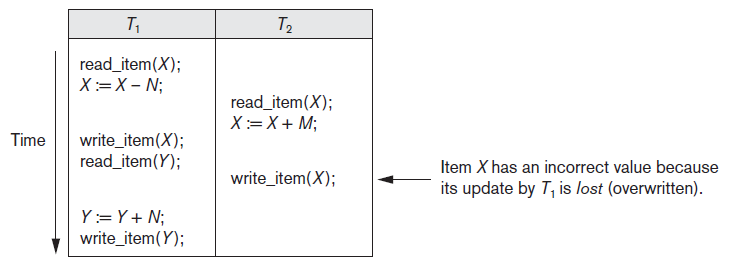
\includegraphics[scale=0.5]{problem_lost_update}



}
\par\end{centering}

\noindent \begin{centering}
\subfloat[Dirty Read]{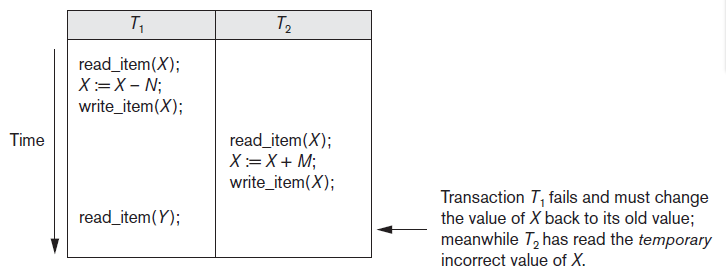
\includegraphics[scale=0.5]{problem_dirty_read}

}
\par\end{centering}

\noindent \begin{centering}
\subfloat[Incorrect Summary]{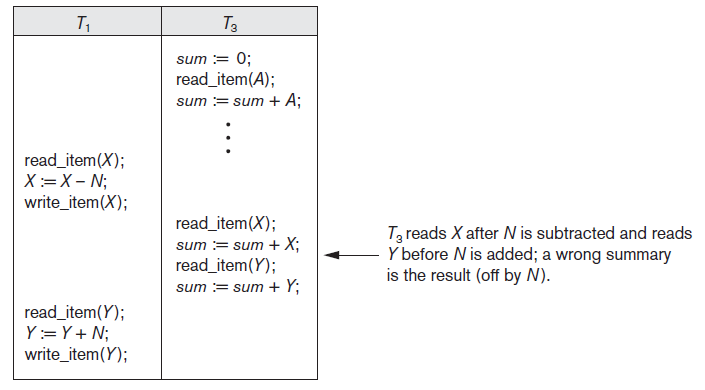
\includegraphics[scale=0.5]{problem_incorrect_summary}}
\par\end{centering}

\protect\caption{Probemas de concurrencia}


\end{figure}


\end{enumerate}

\subsection{Atributos de una Transacción}
\begin{itemize}
\item Modo de acceso: \texttt{READ ONLY}, \texttt{READ WRITE}
\item Nivel de \emph{isolation}:


\begin{table}[H]
\noindent \begin{centering}
\begin{tabular}{|>{\centering}p{2cm}|>{\centering}p{3cm}|>{\centering}p{3cm}|>{\centering}p{3cm}|>{\centering}p{3cm}|}
\hline 
\emph{Nivel de isolation} & \multicolumn{4}{c|}{\emph{Tipo de violación que se puede producir para dos transacciones
$T$ y $S$}}\\
\hline 
\hline 
 & \textbf{Escritura sucia} ($T$ escribe el valor $X$ después de que
una transacción $S$ lo escribiera, y $S$ no comitió ni abortó) & \textbf{Lectura Sucia} ($T$ lee el valor$X$ después de una transacción
$S$ que no comitió ni abortó) & \textbf{Lectura No Repetible} ($T$ lee el valor $X$, luego $S$
lo actualiza, luego $T$ lee $X$ y es un nuevo valor) & \textbf{\emph{Phantoms}} ($T$ lee varios datos que cumplen una condición,
luego $S$ agrega un dato que también lo verifica. Si $T$ lee de
nuevo, encontrará un nuevo dato que antes no estaba) \tabularnewline
\hline 
\emph{READ UNCOMMITTED} & No & Si & Si & Si \tabularnewline
\hline 
\emph{READ COMMITTED} & No & No & Si & Si \tabularnewline
\hline 
\emph{REPEATABLE READ} & No & No & No & Si \tabularnewline
\hline 
\emph{SERIALIZABLE} & No & No & No & No \tabularnewline
\hline 
\end{tabular}
\par\end{centering}

\protect\caption{Violaciones que se pueden producir en cada nivel}


\end{table}


\end{itemize}

\section{Schedules de Transacciones}

\begin{figure}[H]
\noindent \begin{centering}
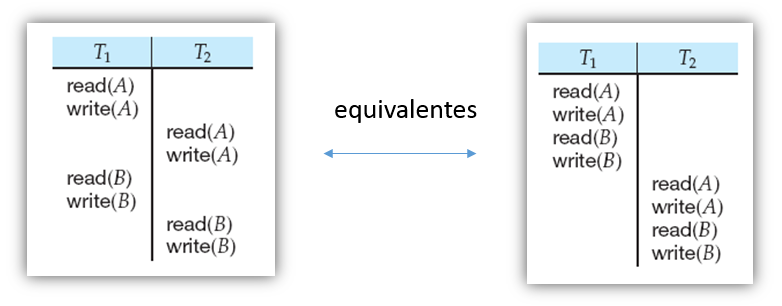
\includegraphics[scale=0.5]{schedules_equivalentes}
\par\end{centering}

\protect\caption{\emph{Schedules} equivalentes}


\end{figure}
\begin{figure}[H]
\noindent \begin{centering}
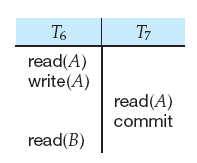
\includegraphics{schedule_no_recuperable}
\par\end{centering}

\protect\caption{\emph{Schedule} no recuperable}
\end{figure}

\begin{description}
\item [{\emph{Schedule}}] ordenamiento cronológico de las operaciones de
$n$ transacciones. Se pueden intercalar operaciones de distintas
transacciones, pero las operaciones de una transacción se deben ejecutar
en forma secuencial.


Un \emph{schedule} es \textbf{recuperable} si, para cada par de transacciones
$T_{i}$ y $T_{j}$ tal que $T_{j}$ lee un ítem de dato previamente
escrito por $T_{i}$, el \texttt{commit} de $T_{i}$ aparece \emph{antes}
del \texttt{commit} de $T_{j}$. 


Un \emph{schedule}\textbf{ }es\textbf{ sin cascada} (\textbf{\emph{avoids
cascading rollback}}\textbf{, AVR}) si, para cada par de transacciones
$T_{i}$ y $T_{j}$ tal que $T_{j}$ lee un ítem de dato previamente
escrito por $T_{i}$, el \texttt{commit} de $T_{i}$ aparece \emph{antes}
del \texttt{read} de $T_{j}$. 


Un \emph{schedule} que usa \emph{locks }es \textbf{estricto} si cada
transacción commitea o aborta, y luego libera todos sus \emph{locks}
exclusivos.


\noindent \begin{center}
estricto $\implies$sin cascada $\implies$recuperable
\par\end{center}


\noindent \begin{center}
estricto $\implies$serializable
\par\end{center}


\begin{figure}[H]
\noindent \begin{centering}
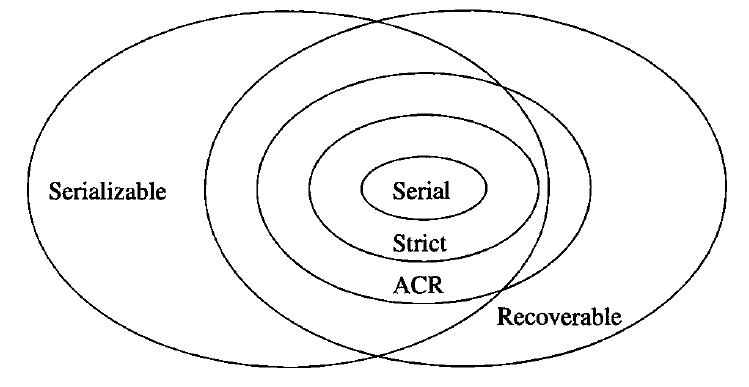
\includegraphics[scale=0.5]{relacion_schedules}
\par\end{centering}

\protect\caption{Relación de \emph{schedules}}


\end{figure}


\item [{Conflicto}] dos \emph{operaciones} en un \emph{schedule} entran
en conflicto cuando se cumplen todas las condiciones siguientes:

\begin{enumerate}
\item Corresponden a distintas transacciones
\item Acceden al mismo ítem de dato $X$
\item Al menos una de esas operaciones es \texttt{escribir(X)}
\end{enumerate}

Dicho de otra forma, están en conflicto cuando, si alteramos el orden
de ejecución, cambia el resultado final de $X$.

\end{description}
Un schedule es \textbf{serial} cuando ejecuta primero todas las operaciones
de $T_{1}$, luego todas las operaciones de $T_{2}$, ..., y finalmente
todas las operaciones de $T_{n}$. Cualquier esquema serial preserva
la consistencia de la base de datos.

Un \emph{schedule} es \textbf{serializable} cuando es equivalente
a algún \emph{schedule} serial con las mismas transacciones.

Dos \emph{schedules} son \textbf{conflicto-equivalentes} si el orden
de las operaciones en conflicto es la misma en ambos. Es decir, si
podemos transformar uno en el otro mediante una secuencia de \emph{swaps}
de acciones adyacentes que no están en conflicto.

\begin{figure}[H]
\noindent \begin{centering}
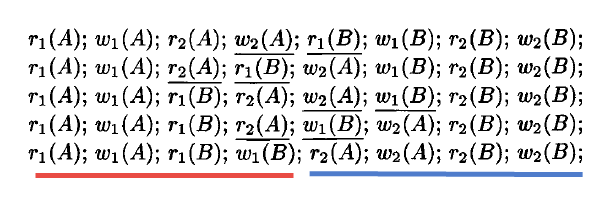
\includegraphics[scale=0.6]{conflicto_serializable}
\par\end{centering}

\protect\caption{Convirtiendo un schedule conflicto-serializable en uno serial mediante
\emph{swaps} de acciones adyacentes. A cada paso están subrayadas
las acciones a punto de ser \emph{swappeadas}}


\end{figure}


Un \emph{schedule} es \textbf{conflicto-serializable} si es conflicto-equivalente
a algún \emph{schedule} serial.

\[
Conflicto\, serializable\implies Serializable
\]


Para verificar si un \emph{schedule $S$ }es conflicto-serializable
se utiliza un grafo dirigido $G=(N,E)$:
\begin{itemize}
\item $N$ es el conjunto de transacciones $\left\{ T_{1},T_{2},\ldots,T_{n}\right\} $
que forman el \emph{schedule}
\item $E$ es el conjunto de aristas de la forma $T_{i}\to T_{j}$. Cada
arista significa que $T_{i}$ debe preceder a $T_{j}$ en cualquier
\emph{schedule} serial equivalente a $S$
\end{itemize}
\begin{algorithm}[H]
\begin{lstlisting}
Entrada: schedule S
Salida: "verdadero" si es conflicto serializable

	para cada transaccion Ti en S:
		crear un nodo Ti en el grafo de precedencia
	para cada caso donde Ti ejecuta READ(X) y luego Tj ejecuta WRITE(X):
		agregar una arista (Ti -> Tj) en el grafo de precedencia
	para cada caso donde Ti ejecuta WRITE(X) y luego Tj ejecuta READ(X):
		agregar una arista (Ti -> Tj) en el grafo de precedencia
	para cada caso donde Ti ejecuta WRITE(X) y luego Tj ejecuta WRITE(X):
		agregar una arista (Ti -> Tj) en el grafo de precedencia
	
	si el grafo es aciclico:
		devolver "verdadero"
	si el gafo es ciclico:
		devolver "falso"
\end{lstlisting}


\protect\caption{Verificación de serializabilidad de un \emph{schedule}}
\end{algorithm}


Si el grafo de precedencia es acíclico, el \emph{schedule} serial
equivalente puede construirse utilizando un \textbf{orden topológico
}de la siguiente forma: siempre que exista una arista $T_{i}\to T_{j}$,
$T_{i}$ debe preceder a $T_{j}$ en el \emph{schedule }serial.

En la práctica, los DBMS no utilizan este algoritmo para garantizar
la serializabilidad (porque habría que verificarlo para cada \emph{schedule}).


\section{Protocolos de Control de Concurrencia: Protocolo de Locking}

Una forma de garantizar el aislamiento de transacciones y prevenir
comportamiento no serializable es mediante el uso de \emph{locks}.
Notar que este mecanismo no funciona bien cuando los \emph{locks}
se mantienen durante días, o cuando las decisiones humanas son parte
de una transacción.
\begin{description}
\item [{\emph{Lock}}] variable que se asocia a un ítem de dato. Describe
el estado del ítem con respecto a las posibles operaciones que pueden
aplicarse a el. Generalmente hay un \emph{lock} por item de dato.


Tipos de \emph{locks}:
\begin{enumerate}
\item \textbf{Binarios}: pueden tener dos valores: \emph{locked} (1) o \emph{unlocked}
(0). Un \emph{lock} binario impone la exclusión mutua en el item de
dato asociado, porque solo puede haber a lo sumo una transacción con
un lock para un mismo dato.


El registro de este tipo de \emph{lock} tiene la forma \texttt{<Item
de dato, LOCK, Transacción con lock>}


Reglas que deben aplicarse a cada transacción:
\begin{enumerate}
\item \texttt{lock(X)} antes de cualquier\texttt{ leer(X) }o\texttt{ escribir(X)}
\item \texttt{unlock(X)} después de \textbf{todos} los \texttt{leer(X)}
y \texttt{escribir(X)}
\item no se permite ejecutar \texttt{lock(X)} si ya se tiene un \emph{lock}
de X
\item no se permite ejecutar \texttt{unlock(X)} si no se tiene el \emph{lock}
de X
\end{enumerate}
\item \textbf{Compartidos/Exclusivos (Lectura/Escritura)}: es más laxo que
los \emph{locks} binarios porque permite que varias transacciones
que solo van a ejecutar \texttt{leer(X)} tengan acceso a X. El \emph{lock}
puede tener dos valores: \emph{read-locked }o \emph{write-locked}.

\begin{itemize}
\item \textbf{Lock exclusivo}: puede leer y escribir el dato $X$.
\item \textbf{Lock compartido}: puede leer pero no puede escribir $X$.
\end{itemize}

El registro este tipo de \emph{lock} tiene la forma \texttt{<Item
de dato, LOCK, \# de lecturas, Transaccion(es) con lock>}


Reglas que deben aplicarse a cada transacción:
\begin{enumerate}
\item \texttt{read\_lock(X)} o \texttt{write\_lock(X)} antes de cualquier
$leer(X)$
\item \texttt{write\_lock(X)} antes de cualquier $escribir(X)$
\item luego de todos los $leer(X)$ y $escribir(X)$, ejecutar $unlock(X)$
\item si ya tiene un \emph{lock} (compartido o exclusivo) de $X$, no se
puede ejecutar ni \texttt{read\_lock(X)} ni \texttt{write\_lock(X)}
\item no se permite ejecutar $unlock(X)$ si no se tiene un \emph{lock}
de $X$ (compartido o exclusivo)
\end{enumerate}
\end{enumerate}

Problemas con el uso de \emph{locks}:
\begin{enumerate}
\item El uso por sí solo de \emph{locks} no garantiza la serializabilidad
de \emph{schedules}.


\begin{figure}[H]
\noindent \begin{centering}
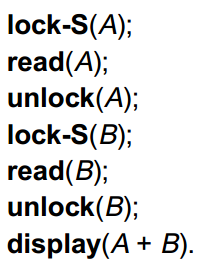
\includegraphics[scale=0.6]{lock_serializability}
\par\end{centering}

\protect\caption{El uso de \emph{locks} no garantiza la serializabilidad. Si se produce
una actualización a $A$ entre $unlock(A)$ y $lock(B)$, \textbf{$A+B$
}sería incorrecto}


\end{figure}


\item \textbf{\emph{Deadlock}}: ocurre cuando cada transacción en un \emph{schedule}
está esperando que se libere un \emph{lock} que fue adquirido por
otra transacción del \emph{schedule.}


Para detectar y/o prevenir un \emph{deadlock}, el gestor de concurrencia
puede mantener un \textbf{grafo de espera}. Cuando una transacción
$T$ está esperando a que la transacción $S$ libere un \emph{lock},
se dibuja una arista $T\to S$. Cuando $S$ libera el \emph{lock},
la arista se borra. El deadlock se detecta cuando el grafo es cíclico.


Cuando ocurre un \emph{deadlock}, el sistema debe ejecutar el \emph{rollback}
de alguna de las dos transacciones, y liberar los \emph{locks} que
ésta poseía.


También se pueden arreglar \emph{deadlocks} especificando un \emph{timeout}
para cada transacción. Si se ejecutan por más tiempo que este \emph{timeout},
es abortada y sus \emph{locks} se liberan.

\item \textbf{\emph{Starvation}}: ocurre cuando una transacción se queda
esperando indefinidamente a que se libere un \emph{lock}. Se puede
evitar de la siguiente forma: cuando una transacción $T_{i}$ solicita
un \emph{lock} sobre $X$ en un modo $M$, el gestor de concurrencia
se lo provee si se verifica que:

\begin{enumerate}
\item No hay otra transacción con un \emph{lock }sobre $X$ en un modo que
conflictúe con $M$.
\item No hay otra transacción esperando obtener un \emph{lock }sobre $X$
antes que $T_{i}$
\end{enumerate}
\end{enumerate}
\item [{Lock~de~update}] un \emph{lock} de \emph{update} le da a una
transacción el privilegio para leer $X$, pero \textbf{no }para escribirlo.
Sin embargo, este tipo de \emph{lock }se puede actualizar a un \emph{lock}
exclusivo más tarde.
\item [{Matriz~de~compatibilidad~de~locks}] se puede otorgar un \emph{lock}
de tipo $C$ si y solo si, para cada fila $R$ tal que ya se otorgó
a otra transacción un lock de tipo $R$, hay un ``Si'' en la columna
$C$.
\end{description}
\begin{table}[H]
\subfloat[Para locks compartidos y exclusivos]{\noindent \begin{centering}
\begin{tabular}{|l|c|c|c|}
\cline{3-4} 
\multicolumn{1}{l}{} &  & \multicolumn{2}{c|}{Se solicita un lock de tipo....}\\
\cline{3-4} 
\multicolumn{1}{l}{} &  & Exclusivo & Compartido\\
\hline 
\multirow{2}{*}{Se otorgó un lock de tipo...} & Exclusivo & No & No\\
\cline{2-4} 
 & Compartido & No & Si\\
\hline 
\end{tabular}
\par\end{centering}

}

\subfloat[Para locks compartidos, exclusivos y de actualización]{\noindent \begin{centering}
\begin{tabular}{|c|c|c|c|c|}
\cline{3-5} 
\multicolumn{1}{c}{} &  & \multicolumn{2}{c}{Se solicita un \emph{lock} de tipo....} & \\
\cline{3-5} 
\multicolumn{1}{c}{} &  & Exclusivo & Compartido & Actualización\\
\hline 
\multirow{3}{*}{Se otorgó un \emph{lock} de tipo...} & Exclusivo & No & No & No\\
\cline{2-5} 
 & Compartido & No & Si & Si\\
\cline{2-5} 
 & Actualización & No & No & No\\
\hline 
\end{tabular}
\par\end{centering}

}

\protect\caption{Ejemplos de matrices de compatibilidad}


\end{table}

\begin{description}
\item [{\emph{Lock~table}}] tabla que utiliza el gestor de concurrencia
para almacenar el estado de los \emph{locks }activos.


Para cada ítem de dato con \emph{locks} activos, mantiene una lista
de transacciones que solicitaron el \emph{lock}, en el orden en que
llegaron los pedidos. Se registra qué transacción es y qué modo de
\emph{lock }solicitó. También se registra si el \emph{lock} le fue
concedido.

\end{description}
\begin{figure}[H]
\noindent \begin{centering}
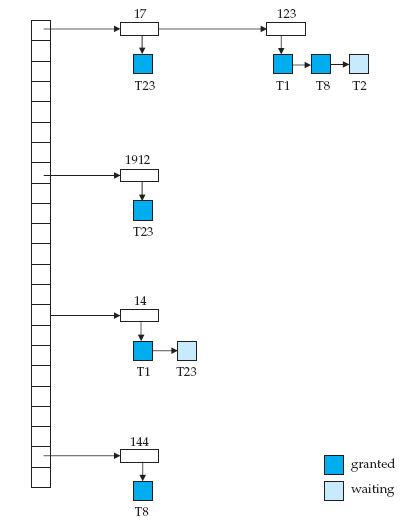
\includegraphics[scale=0.4]{lock_table}
\par\end{centering}

\protect\caption{\emph{Lock table}}


\end{figure}



\subsection{Protocolo de dos fases (\emph{two-phase locking)}}

Una transacción cumple con el protocolo \textbf{\emph{two-phase locking}}\textbf{
(2PL)} si todas las operaciones de \emph{lock} (\texttt{read\_lock},
\texttt{write\_lock}) preceden al primer \emph{unlock} de la transacción.
Se dice entonces que la transacción se divide en dos fases: la creciente
(donde se adquieren los \emph{locks}) y la decreciente (donde se liberan
los \emph{locks}).

Si cada transacción de un \emph{schedule} cumple el protocolo 2PL,
se garantiza que el \emph{schedule} es serializable. De hecho, las
transacciones se pueden ordenar de acuerdo a sus \emph{lock points}
(el punto donde termina la fase creciente).

Este protocolo limita la cantidad de concurrencia que se permite,
porque una transacción no puede liberar un \emph{lock} hasta que haya
adquirido un \emph{lock} para todos los demás ítems, y entonces puede
haber muchas otras transacciones esperando que se libere el primer
\emph{lock}. Además, no se previene el \emph{deadlock}, ni los \emph{rollbacks}
en cascada.

\begin{figure}[H]
\noindent \begin{centering}
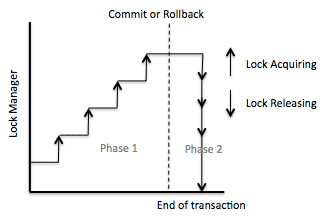
\includegraphics[scale=0.7]{2PL}
\par\end{centering}

\protect\caption{2PL}


\end{figure}
\begin{figure}[H]
\noindent \begin{centering}
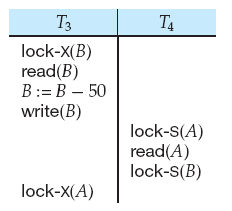
\includegraphics[scale=0.7]{2pl_deadlock}
\par\end{centering}

\protect\caption{Schedule 2PL con \emph{deadlock}}
\end{figure}
\begin{figure}[H]
\noindent \begin{centering}
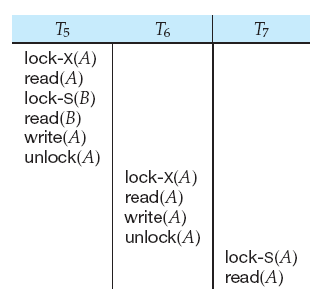
\includegraphics[scale=0.5]{2pl_cascading_rollback}
\par\end{centering}

\protect\caption{Schedule 2PL con \emph{cascading rollback }si $T_{5}$ falla al final
de todo}
\end{figure}


Para prevenir el problema de \emph{deadlock}, este protocolo puede
ampliarse y exigir que las transacciones adquieran por adelantado
todos los \emph{locks} que se necesitan; si un \emph{lock} no se puede
conseguir, no se adquiere ninguno. Esto limita aún más la concurrencia.

Para prevenir el problema de \emph{rollbacks} en cascada, existe el
protocolo\textbf{ 2PL estricto}. Este modo, además de requerir lo
mismo que 2PL, requiere que todos los \emph{locks} exclusivos adquiridos
por una transacción se mantengan hasta que la misma ejecute \emph{commit.}


\subsection{Protocolo de árbol}
\begin{description}
\item [{Protocolo~de~árbol}] protocolo especializado para transacciones
que acceden a datos en forma de árbol (ejemplo: un índice B). El protocolo
viola 2PL, pero utiliza el hecho de que acceder a elementos debe ser
hacia abajo para garantizar serializabilidad.
\end{description}
Si una transacción quiere insertar un registro, debería adquirir un
\emph{lock} exclusivo de la raíz, ergo de todo el árbol, y por ende
estaría bloqueando a todas las demás transacciones.

Puede aprovecharse la estructura de árbol del índice de la siguiente
forma:
\begin{itemize}
\item Cuando se adquiere un \emph{read\_lock} en un nodo hijo, el \emph{lock}
del nodo padre puede liberarse porque no se usará más.
\item Cuando se adquiere un \emph{write\_lock} en un nodo hoja (para realizar
una inserción), se debe adquirir un \emph{lock }exclusivo en el nodo
hoja.
\end{itemize}
Utilizar la técnica de \textbf{\emph{index locking}} soluciona el
problema de registros \emph{phantom}.

El protocolo de árbol garantiza un orden serial en las transacciones.
El orden de precedencia se define así: si $T_{i}$ y $T_{j}$ adquieren
un \emph{lock }sobre $X$ y $T_{i}$ adquiere el \emph{lock }primero,
entonces $T_{i}\to T_{j}$.

\begin{algorithm}[H]
\begin{enumerate}
\item El primer lock de una transacción puede hacerse sobre cualquier nodo
del árbol.
\item Los locks subsiguientes pueden otorgarse sólo si se posee un lock
sobre el nodo padre.
\item Se puede ejecutar \emph{unlock} de un nodo en cualquier momento.
\item No se puede adquirir \emph{lock} de un nodo 2 veces, incluso cuando
se tiene un \emph{lock }sobre el nodo padre.
\end{enumerate}
\protect\caption{Protocolo de árbol}


\end{algorithm}


\pagebreak{}


\part{Técnicas de Recuperación}


\section{Necesidad de Recuperación}

Tipos de fallas que pueden ocurrir:
\begin{enumerate}
\item Fallas de la computadora: por ejemplo, una desconexión en la red
\item Fallas de transacciones: por ejemplo, una transacción que intenta
dividir por cero
\item Errores locales: por ejemplo, una transacción que no encuentra datos
\item Aplicación de procedimientos de control de concurrencia: por ejemplo,
una transacción abortada porque viola la serializabilidad o para resolver
un estado de \emph{deadlock}
\item Fallas del disco
\item Catástrofes
\end{enumerate}
Los algoritmos de recuperación tienen dos partes:
\begin{enumerate}
\item Acciones que se toman durante el procesamiento normal de transacciones,
para asegurar que, en caso de falla, se dispone de suficiente información
para recuperar
\item Acciones que se toman después de una falla para devolver la base de
datos a un estado consistente.
\end{enumerate}
Idealmente, la base de datos en disco debería contener, para cada
ítem de dato, el último valor escrito por una transacción que ejecutó
\emph{commit}.

En la práctica, la base de datos podría:
\begin{itemize}
\item Contener valores escritos por transacciones no commiteadas
\item No contener valores escritos por transacciones commiteadas
\end{itemize}

\section{Archivo de Log}

La base de datos se almacena en disco. Éste está formado por bloques.
Como todos los bloques no caben en memoria principal, se necesita
una forma de trabajar con la base de datos en memoria. Por ende, se
necesita una forma de organizar los bloques en memoria y luego copiarlos
en el disco (\emph{flush}).

\begin{figure}[H]
\noindent \begin{centering}
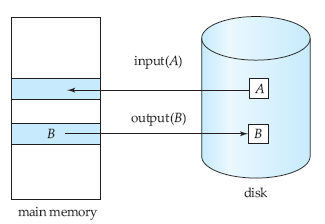
\includegraphics{input_output}
\par\end{centering}

\protect\caption{Operaciones sobre bloques}


\end{figure}


Para alcanzar el objetivo de transacciones atómicas, primero se debe
guardar en disco información sobre las modificaciones, sin modificar
la base de datos en sí. Para eso se utiliza un archivo de \emph{log}.
Este archivo permite: 
\begin{itemize}
\item Deshacer (\emph{undo}) cambios hechos por transacciones que deben
ser abortadas
\item Rehacer (\emph{redo}) cambios hechos por transacciones que ejecutaron
\emph{commit} pero cuyos cambios no fueron almacenados en la base
de datos en disco.\end{itemize}
\begin{description}
\item [{Log}] archivo secuencial al que solo se le pueden agregar registros.
\end{description}
Decimos que una transacción ejecutó \textbf{commit} cuando su registro
\texttt{{[}commit,T{]} }fue almacenado en disco. Si hay una falla
luego de esto, se ejecuta un \textbf{redo}. Si hay una falla antes
de esto, se hace \textbf{\emph{undo.}}
\begin{itemize}
\item \textbf{Redo} debe hacerse en el orden en el que los cambios fueron
hechos originalmente.
\item \textbf{Undo }escribe registros especiales llamados ``redo-only'',
que no tienen el valor viejo del item de dato. Al finalizar las escrituras,
se escribe un registro \texttt{<abort,T> }para indicar que el \emph{undo
}finalizó.
\end{itemize}

\subsection{Checkpoints}

Cuando se produce una caída del sistema, hay que consultar el \emph{log}
para determinar aquellas transacciones que deben rehacerse o deshacerse.
En principio, habría que buscar en todo el \emph{log} para determinar
esta información. Hay dos grandes dificultades con este enfoque: 
\begin{enumerate}
\item El proceso de búsqueda lleva mucho tiempo. 
\item La mayor parte de las transacciones ya han escrito sus actualizaciones
en la base de datos. 
\end{enumerate}
Para reducir este tipo de gastos generales, se usan los \textbf{\emph{checkpoints}}.
La periodicidad con que se ejecutan \emph{checkpoints} la decide el
administrador de base de datos.


\subsubsection{Checkpoints bloqueantes}

Se describe a continuación un esquema de control simple que (a) no
permite realizar ningún cambio mientras la operación está en curso,
y (b) se escriben en disco todos los \emph{buffers} en memoria modificados. 

\begin{algorithm}[H]
\emph{1. Stop accepting new transactions.}

\emph{2. Wait until all currently active transactions commit or abort
and have written a }\texttt{\emph{COMMIT}}\emph{ or }\texttt{\emph{ABORT}}\emph{
record on the log. }

\emph{3. Flush the log to disk. }

\emph{4. Write a log record }\texttt{\emph{<CHECKPOINT>}}\emph{, and
flush the log again. }

\emph{5. Resume accepting transactions.}

\protect\caption{Checkpoint bloqueante en un log UNDO}


\end{algorithm}



\subsubsection{Checkpoints no bloqueantes}

\begin{algorithm}[H]
\emph{1. Write a log record }\texttt{\emph{<START CHECKPOINT (T1,
... , Tk)>}}\emph{. Here, $T_{1},\ldots,T_{k}$ are the identifiers
for all the active transactions (i.e., transactions that have not
yet committed and written their changes to disk). }

\emph{2. Flush the log.}

\emph{3. Wait until all of $T_{1},\ldots,T_{k}$ commit or abort,
but do not prohibit other transactions from starting. }

\emph{4. When all of $T_{1},\ldots,T_{k}$ have completed, write a
log record }\texttt{\emph{<END CHECKPOINT>}}\emph{. }

\emph{5. Flush the log.}

\protect\caption{Checkpoint no bloqueante en un log UNDO}
\end{algorithm}


\begin{algorithm}[H]
\emph{1. Write a log record }\texttt{\emph{<START CHECKPOINT (T1,
... , Tk)>}}\emph{. Here, $T_{1},\ldots,T_{k}$ are the identifiers
for all the active transactions (i.e., transactions that have not
yet committed). }

\emph{2. Flush the log.}

\emph{3. Write to disk all database elements that were written to
buffers but not yet to disk by transactions that had already committed
when the <START CHECKPOINT> record was written to the log.}

\emph{4. Write a log record }\texttt{\emph{<END CHECKPOINT>}}\emph{. }

\emph{5. Flush the log.}

\protect\caption{Checkpoint no bloqueante en un log REDO}
\end{algorithm}


\begin{algorithm}[H]
\emph{1. Write a log record }\texttt{\emph{<START CHECKPOINT (T1,
... , Tk)>}}\emph{. Here, $T_{1},\ldots,T_{k}$ are the identifiers
for all the active transactions (i.e., transactions that have not
yet committed). }

\emph{2. Flush the log.}

\emph{3. Write to disk }\textbf{\emph{all}}\emph{ buffers that are
dirty (not just those written by committed transactions)}

\emph{4. Write a log record }\texttt{\emph{<END CHECKPOINT>}}\emph{. }

\emph{5. Flush the log.}

\protect\caption{Checkpoint no bloqueante en un log UNDO/REDO}
\end{algorithm}



\section{Protocolos de Recuperación}
\begin{itemize}
\item Para fallas de tipo 5 y 6, se necesita haber grabado con anterioridad
un \emph{backup} de la base de datos y reconstruir la misma con el
archivo de log hasta el momento de la falla.
\item Para fallas de tipo 1 a 4, existen dos técnicas de recuperación:

\begin{itemize}
\item \textbf{\emph{Deferred update}}


Las transacciones y el manejador de buffers obedecen 1 regla:
\begin{itemize}
\item \textbf{Write-Ahead Logging (WAL)}:\textbf{ }se deben grabar en disco
todos los registros de log sobre las actualización (incluyendo \texttt{<UPDATE
T,X,Nuevo\_valor>} y \texttt{<COMMIT T>}), y luego actualizar $X$
en disco.
\end{itemize}

Tipos de registros:
\begin{itemize}
\item \texttt{<START T>}
\item \texttt{<COMMIT T>}
\item \texttt{<ABORT T>}
\item \texttt{<UPDATE T,X,Valor\_Nuevo>}
\end{itemize}

\begin{algorithm}[H]
\begin{lstlisting}
transacciones_commiteadas = identificarlas
transacciones_incompletas = identificarlas

desde el comienzo del log hasta el fin:
	si hay un registro <UPDATE <T,X,Valor_Nuevo>:
		si T esta en ``transacciones_commiteadas'':
			escribir ``Valor_Nuevo'' en X
		si no:
			no hacer nada

para cada T en ``transacciones_incompletas'':
	escribir <ABORT T>

flush_log()
\end{lstlisting}


\protect\caption{Procedimiento de recuperación \textbf{REDO }sin checkpoints}
\end{algorithm}



\begin{algorithm}[H]
\begin{lstlisting}
transacciones_commiteadas = identificarlas
transacciones_incompletas = identificarlas

desde el comienzo del log hasta el fin:
	si hay un registro <UPDATE <T,X,Valor_Nuevo>:
		si T esta en "transacciones_commiteadas":
			escribir "Valor_Nuevo" en X
		si no:
			no hacer nada
	si el ultimo registro de checkpoint es <END CHECKPOINT>:
		// se debe mirar el log hasta el <START Ti> que se ejecuto primero
	si el ultimo registro de checkpoint es <START CHECKPOINT T1,...,TK>:
		// la caida se produjo durante el checkpointing
		// buscar el registro <END CHECKPOINT> anterior y su par <START CHECKPOINT S1,...,SK>
		// rehacer todas las transacciones commiteadas que empezaron despues de ese START 
		//	o son Si
		// (si no hay, rehacer desde el principio del log)

para cada T en transacciones_incompletas:
	escribir <ABORT T>

flush_log()
\end{lstlisting}


\protect\caption{Procedimiento de recuperación \textbf{REDO }con checkpoints no bloqueantes}
\end{algorithm}



El algoritmo anterior puede ser más eficiente si se ejecuta, para
cada item de dato, sólo el último REDO existente (porque todos los
anteriores serían sobrescritos por éste).


Este mecanismo garantiza:
\begin{itemize}
\item Que no se deban hacer \emph{rollbacks} de transacciones (porque las
mismas sólo escriben en la base de datos luego de ejecutar commit)
\item Que no se deban hacer \emph{rollbacks} en cascada (porque los ítems
tienen locks que no permiten leerlos antes de que una transacción
que los escribió no ejecute commit)
\end{itemize}
\item \textbf{\emph{Immediate update}}: a su vez tiene dos variantes:

\begin{enumerate}
\item \textbf{UNDO/REDO}: Las transacciones y el manejador de buffer obedecen
1 regla:

\begin{itemize}
\item Si la transacción $T$ modifica el ítem de dato $X$, el registro
de log \texttt{<UPDATE T,X,Valor\_Viejo,Valor\_Nuevo>} debe ser escrito
al disco \textbf{antes} que el ítem $X$ sea escrito al disco.
\end{itemize}

Tipos de registros:
\begin{itemize}
\item \texttt{<START T>}
\item \texttt{<COMMIT T>}
\item \texttt{<ABORT T>}
\item \texttt{<UPDATE T,X,Valor\_Viejo,Valor\_Nuevo>}
\end{itemize}

\begin{algorithm}[H]
\begin{lstlisting}
mantener dos listas de transacciones:
1) transacciones commiteadas desde el ultimo checkpoint
2) transacciones activas

ejecutar REDO de todos los ESCRIBIR de las transacciones de la primera lista, 
en el orden en que fueron escritos en el log

ejecutar UNDO de todos los ESCRIBIR de las transacciones de la segunda lista, 
en el orden inverso en que fueron escritos en el log
\end{lstlisting}


\protect\caption{Procedimiento de recuperación \textbf{UNDO/REDO}}
\end{algorithm}


\item \textbf{UNDO}: Las transacciones y el manejador de buffer obedecen
2 reglas:

\begin{enumerate}
\item Si la transacción $T$ modifica el ítem de dato $X$, el registro
de log \texttt{<UPDATE T,X,Valor\_Viejo>} debe ser escrito al disco
\textbf{antes} que el ítem $X$ sea escrito al disco.
\item \textbf{\emph{Force Log at Commi}}\textbf{t (FLC}): si la transacción
ejecuta commit, los ítems de datos actualizados por la transacción
se deben escribir en el disco, y luego el registro de log \texttt{<COMMIT
T>} debe ser escrito al disco.
\end{enumerate}

Tipos de registros:
\begin{itemize}
\item \texttt{<START T>}
\item \texttt{<COMMIT T>}
\item \texttt{<ABORT T>}
\item \texttt{<UPDATE T,X,Valor\_Viejo>}
\end{itemize}

\begin{algorithm}[H]
\begin{lstlisting}
transacciones_completas = {}
transacciones_incompletas = {}

desde el fin del log hasta el comienzo: // o hasta que se encuentre un registro <CHECKPOINT>
	si hay un registro <COMMIT T> o <ABORT T>:
		transacciones_completas += T
	si hay un registro <UPDATE <T,X,Valor_Viejo>:
		si T esta en "transacciones_completas":
			no hacer nada
		sino:
			transacciones_incompletas += T
			escribir "Valor_Viejo" en "X"

para cada T en "transacciones_incompletas":
	escribir <ABORT T>

flush_log()
\end{lstlisting}


\protect\caption{Procedimiento de recuperación \textbf{UNDO }con checkpoint bloqueante}
\end{algorithm}



\begin{algorithm}[H]
\begin{lstlisting}
transacciones_completas = {}
transacciones_incompletas = {}

desde el fin del log: 
	si hay un registro <COMMIT T> o <ABORT T>:
		transacciones_completas += T
	si hay un registro <UPDATE <T,X,Valor_Viejo>:
		si T esta en "transacciones_completas":
			no hacer nada
		sino:
			transacciones_incompletas += T
			escribir "Valor_Viejo" en "X"
	si hay un registro <END CHECKPOINT>:
		// se debe mirar el log hasta el <START CHECKPOINT> correspondiente
	si hay un registro <START CHECKPOINT T1,...,TK> pero no un <END CHECKPOINT>:
		// la caida se produjo durante el checkpointing
		// se debe mirar el log hasta el comienzo de la primera transaccion incompleta

para cada T en "transacciones_incompletas":
	escribir <ABORT T>

flush_log()
\end{lstlisting}


\protect\caption{Procedimiento de recuperación \textbf{UNDO }con checkpoint no bloqueante}
\end{algorithm}


\end{enumerate}
\end{itemize}
\end{itemize}
Es necesario que las operaciones de UNDO y REDO sean \textbf{idempotentes}:
ejecutarlas muchas veces debe ser igual a ejecutarlas muchas veces.
De hecho, todo el proceso de recuperación debe ser idempotente para
garantizar que si existe una falla durante la recuperación de una
falla, la misma se pueda recuperar también.

Es necesario que el DBMS mantenga:
\begin{itemize}
\item Lista de transacciones activas
\item Lista de transacciones que ejecutaron commit
\item Lista de transacciones abortadas desde el último checkpoint
\end{itemize}
\begin{figure}[H]
\subfloat[Log UNDO]{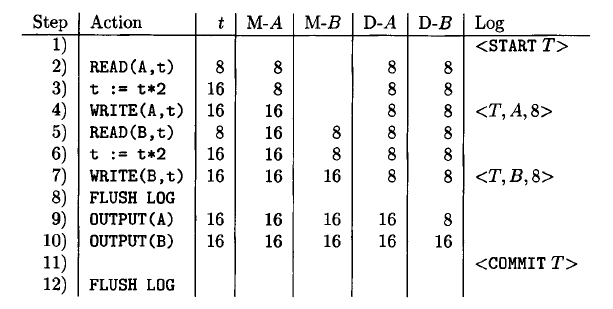
\includegraphics[scale=0.5]{undo_logging}



}\subfloat[Log REDO]{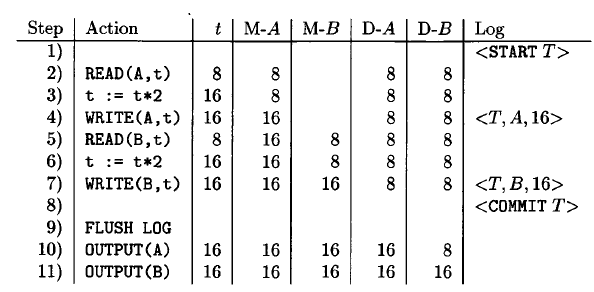
\includegraphics[scale=0.5]{redo_logging}

}

\subfloat[Log UNDO/REDO]{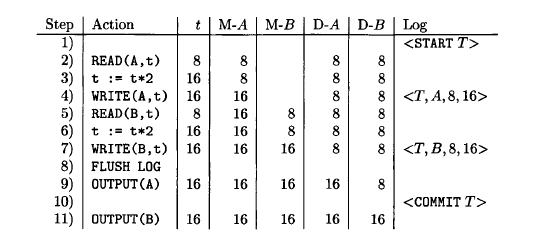
\includegraphics[scale=0.5]{undo_redo_logging}

}\protect\caption{Ejemplos de logs}


\end{figure}


\noindent \begin{center}
\begin{tabular}{|c|c|c|}
\hline 
\texttt{\textbf{UNDO}} & \texttt{\textbf{REDO}} & \texttt{\textbf{UNDO/REDO}}\\
\hline 
\hline 
$Logs\, X\implies Bd\, X\implies Commit\, al\, log$ & $Logs\, X\,\&\, Commit\, al\, log\implies Bd\, X$ & $Log\, X\implies Bd\, X$\\
\hline 
\emph{Immediate update} & \emph{Deferred update} & \emph{Immediate update}\\
\hline 
\end{tabular}
\par\end{center}

% Bibliografía utilizada en el apunte
%\newpage
%\newcommand{\bibliographyname}{Bibliografía} % Defino el nombre de la sección de la bibliografía
%\addcontentsline{toc}{section}{\bibliographyname} % Agrego la bibliografía en el índice
%\renewcommand\refname{\bibliographyname} % Renombro a la bibliografía (por default es 'Referencias')
%\begin{thebibliography}{X}
%	\bibitem{Marsden} \textsc{Jerrold E. Marsden} y \textsc{Anthony J. Tromba}, \textit{Cálculo Vectorial}, tercera edición, Addison-Wesley Iberoamericana, 1991.
%\end{thebibliography}

% Nombres de las personas que han colaborado en la creación del apunte
\colaborador{María Inés Parnisari (maineparnisari@gmail.com)}
\makeseccioncolaboradores % Crea la seccion de colaboradres

% Incluir el historial de cambios
\revision{08/03/2015}{Versión inicial}
\makehistorial

\end{document}
